% Options for packages loaded elsewhere
\PassOptionsToPackage{unicode}{hyperref}
\PassOptionsToPackage{hyphens}{url}
\PassOptionsToPackage{dvipsnames,svgnames,x11names}{xcolor}
%
\documentclass[
  12pt,
  letterpaper,
  DIV=11,
  numbers=noendperiod]{scrreprt}

\usepackage{amsmath,amssymb}
\usepackage{iftex}
\ifPDFTeX
  \usepackage[T1]{fontenc}
  \usepackage[utf8]{inputenc}
  \usepackage{textcomp} % provide euro and other symbols
\else % if luatex or xetex
  \usepackage{unicode-math}
  \defaultfontfeatures{Scale=MatchLowercase}
  \defaultfontfeatures[\rmfamily]{Ligatures=TeX,Scale=1}
\fi
\usepackage{lmodern}
\ifPDFTeX\else  
    % xetex/luatex font selection
  \setmainfont[Scale = MatchLowercase]{Scala Pro}
  \setsansfont[]{Scala Sans Pro}
\fi
% Use upquote if available, for straight quotes in verbatim environments
\IfFileExists{upquote.sty}{\usepackage{upquote}}{}
\IfFileExists{microtype.sty}{% use microtype if available
  \usepackage[]{microtype}
  \UseMicrotypeSet[protrusion]{basicmath} % disable protrusion for tt fonts
}{}
\makeatletter
\@ifundefined{KOMAClassName}{% if non-KOMA class
  \IfFileExists{parskip.sty}{%
    \usepackage{parskip}
  }{% else
    \setlength{\parindent}{0pt}
    \setlength{\parskip}{6pt plus 2pt minus 1pt}}
}{% if KOMA class
  \KOMAoptions{parskip=half}}
\makeatother
\usepackage{xcolor}
\usepackage[left=1.5in,right=1.5in,top=1.78in,bottom=1.78in]{geometry}
\setlength{\emergencystretch}{3em} % prevent overfull lines
\setcounter{secnumdepth}{5}
% Make \paragraph and \subparagraph free-standing
\ifx\paragraph\undefined\else
  \let\oldparagraph\paragraph
  \renewcommand{\paragraph}[1]{\oldparagraph{#1}\mbox{}}
\fi
\ifx\subparagraph\undefined\else
  \let\oldsubparagraph\subparagraph
  \renewcommand{\subparagraph}[1]{\oldsubparagraph{#1}\mbox{}}
\fi


\providecommand{\tightlist}{%
  \setlength{\itemsep}{0pt}\setlength{\parskip}{0pt}}\usepackage{longtable,booktabs,array}
\usepackage{calc} % for calculating minipage widths
% Correct order of tables after \paragraph or \subparagraph
\usepackage{etoolbox}
\makeatletter
\patchcmd\longtable{\par}{\if@noskipsec\mbox{}\fi\par}{}{}
\makeatother
% Allow footnotes in longtable head/foot
\IfFileExists{footnotehyper.sty}{\usepackage{footnotehyper}}{\usepackage{footnote}}
\makesavenoteenv{longtable}
\usepackage{graphicx}
\makeatletter
\def\maxwidth{\ifdim\Gin@nat@width>\linewidth\linewidth\else\Gin@nat@width\fi}
\def\maxheight{\ifdim\Gin@nat@height>\textheight\textheight\else\Gin@nat@height\fi}
\makeatother
% Scale images if necessary, so that they will not overflow the page
% margins by default, and it is still possible to overwrite the defaults
% using explicit options in \includegraphics[width, height, ...]{}
\setkeys{Gin}{width=\maxwidth,height=\maxheight,keepaspectratio}
% Set default figure placement to htbp
\makeatletter
\def\fps@figure{htbp}
\makeatother
\newlength{\cslhangindent}
\setlength{\cslhangindent}{1.5em}
\newlength{\csllabelwidth}
\setlength{\csllabelwidth}{3em}
\newlength{\cslentryspacingunit} % times entry-spacing
\setlength{\cslentryspacingunit}{\parskip}
\newenvironment{CSLReferences}[2] % #1 hanging-ident, #2 entry spacing
 {% don't indent paragraphs
  \setlength{\parindent}{0pt}
  % turn on hanging indent if param 1 is 1
  \ifodd #1
  \let\oldpar\par
  \def\par{\hangindent=\cslhangindent\oldpar}
  \fi
  % set entry spacing
  \setlength{\parskip}{#2\cslentryspacingunit}
 }%
 {}
\usepackage{calc}
\newcommand{\CSLBlock}[1]{#1\hfill\break}
\newcommand{\CSLLeftMargin}[1]{\parbox[t]{\csllabelwidth}{#1}}
\newcommand{\CSLRightInline}[1]{\parbox[t]{\linewidth - \csllabelwidth}{#1}\break}
\newcommand{\CSLIndent}[1]{\hspace{\cslhangindent}#1}

\setlength\heavyrulewidth{0ex}
\setlength\lightrulewidth{0ex}
\usepackage{makecell}
\renewcommand\theadfont{\bfseries}
\KOMAoption{captions}{tableheading}
\makeatletter
\makeatother
\makeatletter
\@ifpackageloaded{bookmark}{}{\usepackage{bookmark}}
\makeatother
\makeatletter
\@ifpackageloaded{caption}{}{\usepackage{caption}}
\AtBeginDocument{%
\ifdefined\contentsname
  \renewcommand*\contentsname{Table of contents}
\else
  \newcommand\contentsname{Table of contents}
\fi
\ifdefined\listfigurename
  \renewcommand*\listfigurename{List of Figures}
\else
  \newcommand\listfigurename{List of Figures}
\fi
\ifdefined\listtablename
  \renewcommand*\listtablename{List of Tables}
\else
  \newcommand\listtablename{List of Tables}
\fi
\ifdefined\figurename
  \renewcommand*\figurename{Figure}
\else
  \newcommand\figurename{Figure}
\fi
\ifdefined\tablename
  \renewcommand*\tablename{Table}
\else
  \newcommand\tablename{Table}
\fi
}
\@ifpackageloaded{float}{}{\usepackage{float}}
\floatstyle{ruled}
\@ifundefined{c@chapter}{\newfloat{codelisting}{h}{lop}}{\newfloat{codelisting}{h}{lop}[chapter]}
\floatname{codelisting}{Listing}
\newcommand*\listoflistings{\listof{codelisting}{List of Listings}}
\makeatother
\makeatletter
\@ifpackageloaded{caption}{}{\usepackage{caption}}
\@ifpackageloaded{subcaption}{}{\usepackage{subcaption}}
\makeatother
\makeatletter
\@ifpackageloaded{tcolorbox}{}{\usepackage[skins,breakable]{tcolorbox}}
\makeatother
\makeatletter
\@ifundefined{shadecolor}{\definecolor{shadecolor}{rgb}{.97, .97, .97}}
\makeatother
\makeatletter
\makeatother
\makeatletter
\makeatother
\ifLuaTeX
  \usepackage{selnolig}  % disable illegal ligatures
\fi
\IfFileExists{bookmark.sty}{\usepackage{bookmark}}{\usepackage{hyperref}}
\IfFileExists{xurl.sty}{\usepackage{xurl}}{} % add URL line breaks if available
\urlstyle{same} % disable monospaced font for URLs
\hypersetup{
  pdftitle={Game Theory as Decision Theory},
  pdfauthor={Brian Weatherson},
  colorlinks=true,
  linkcolor={black},
  filecolor={Maroon},
  citecolor={Blue},
  urlcolor={Blue},
  pdfcreator={LaTeX via pandoc}}

\title{Game Theory as Decision Theory}
\author{Brian Weatherson}
\date{2023-10-18}

\begin{document}
\maketitle
\ifdefined\Shaded\renewenvironment{Shaded}{\begin{tcolorbox}[breakable, frame hidden, boxrule=0pt, interior hidden, sharp corners, borderline west={3pt}{0pt}{shadecolor}, enhanced]}{\end{tcolorbox}}\fi

\renewcommand*\contentsname{Table of contents}
{
\hypersetup{linkcolor=}
\setcounter{tocdepth}{2}
\tableofcontents
}
\bookmarksetup{startatroot}

\hypertarget{preface}{%
\chapter*{Preface}\label{preface}}
\addcontentsline{toc}{chapter}{Preface}

\markboth{Preface}{Preface}

Draft for a book based on my (overly long) paper
\href{https://brian.weatherson.org/gdt/gdt.html}{Gamified Decision
Theory}.

\bookmarksetup{startatroot}

\hypertarget{sec-intro}{%
\chapter{Introduction}\label{sec-intro}}

\hypertarget{sec-ten-features}{%
\section{Ten Features of a Good Decision
Theory}\label{sec-ten-features}}

Textbook versions of game theory embed a distinctive approach to
decision theory. That theory isn't always made explicit, and it isn't
always clear how it handles some cases. But we can extract an
interesting and plausible theory, which I'll call Gamified Decision
Theory (GDT), from these textbooks. I will focus on these ten
characteristics of GDT, with one chapter to come on each.

\begin{enumerate}
\def\labelenumi{\arabic{enumi}.}
\tightlist
\item
  \textbf{Idealised}: GDT is a theory of what ideal deciders do.
\item
  \textbf{Expectationist}: The ideal decider prefers getting more
  expected value to getting less.
\item
  \textbf{Causal}: GDT is a version of Causal Decision Theory (CDT).
\item
  \textbf{Allows Mixtures}: The ideal decider can perform a
  probabilistic mixture of any acts they can perform.
\item
  \textbf{Ratificationist}: The ideal decider endorses the decisions
  they make.
\item
  \textbf{Dual Mandate}: In a dynamic choice, the ideal decider will
  follow a plan that's permissible, and take choices at every stage that
  are permissible.
\item
  \textbf{Indecisive}: GDT sometimes says that multiple options are
  permissible, and they are not equally good.
\item
  \textbf{Selection}: The aim of decision theory is to generate a
  function from possible choices to choice-worthy options, not to
  generate a preference ordering over the options.
\item
  \textbf{Substantive Probability}: The ideal decider has rational
  credences.
\item
  \textbf{Weak Dominance, Once}; The ideal decider will not choose
  weakly dominated options, but they may choose options that would not
  survive iterated deletion of weakly dominated strategies.
\end{enumerate}

This is not going to be a work of exegesis, poring over game theory
texts to show that they really do endorse all ten of these. In fact it
wouldn't take much work to show that they endorse 1-5, so the work
wouldn't be worth doing. And while some textbooks endorse 9 and 10, it
would take a lot more investigative work than I'm going to do here to
show that anything like a majority of them do. It would be interesting,
but not obviously a philosophical question, to see what proportion
endorse 6, 7 or 8. But I'm going to set those interpretative questions
aside.

What I do want to argue is that you can find some support for all of
these in some game theory textbooks, and that combined they produce a
plausible decision theory. While the textbooks don't all agree, for
simplicity I'm going to focus on one book: Giacomo Bonanno's \emph{Game
Theory} (\protect\hyperlink{ref-Bonanno2018}{Bonanno 2018}). This book
has two important virtues: it is philosophically deep, and it is
available for free. It isn't hard to find a game theory text with one or
other of these virtues, but few have both. So it will be our primary
guide in what follows, along with some primary sources (most of which
are referenced in that book).

\hypertarget{sec-intro-demons}{%
\section{Demons}\label{sec-intro-demons}}

A lot of contemporary philosophical decision theory revolves around what
to do if there is a certain kind of demon around. Following Nozick
(\protect\hyperlink{ref-Nozick1969}{1969}), such a demon is typically
taken to be arbitrarily good at predicting what a human deliberator will
do. I'll call our arbitrary deliberator Chooser, and a typical demon
Demon. Whenever X is a choice Chooser can make, I'll use PX to mean that
Demon predicts Chooser chooses X. It's not so common to have problems
where there are two such demons around, but I'll make heavy use of them,
and in such cases I'll be clear about whether PX means that the first or
the second demon predicted that Chooser will do X. These are
predictions, and we assume that causation runs from past to future, so
what Chooser does has no causal impact on what Demon predicts.

I'm squeamish about assigning probability 1 to predictions that are
causally isolated from the thing being predicted; I have reductionist
enough views about causation to think that if a prediction is correct
with probability 1, that raises questions about whether causation does
really run from past to future in this case. So I prefer to say that
Demon is correct with a probability close enough to 1 that it doesn't
matter for the purposes of the problem being analysed. But this
squeamishness, and the associated reductionism about causation, is not
part of GDT. If you're happy with having causally isolated demons who
are correct with probability 1, everything else I say should be
acceptable. Indeed, some of the reasoning goes through even more
smoothly with perfectly accurate, but causally isolated, demons.

A generic binary choice problem involving Chooser and Demon can be
depicted by Table~\ref{tbl-gen-dem-problem-text}.

\hypertarget{tbl-gen-dem-problem-text}{}
\begin{longtable}[]{@{}ccc@{}}
\caption{\label{tbl-gen-dem-problem-text}The generic demonic decision
problem.}\tabularnewline
\toprule\noalign{}
& \textbf{PA} & \textbf{PB} \\
\midrule\noalign{}
\endfirsthead
\toprule\noalign{}
& \textbf{PA} & \textbf{PB} \\
\midrule\noalign{}
\endhead
\bottomrule\noalign{}
\endlastfoot
\textbf{A} & \emph{x} & \emph{y} \\
\textbf{B} & \emph{z} & \emph{w} \\
\end{longtable}

Chooser selects A or B, Demon predicts the choice, and there are four
possible outcomes. Slightly more perspicuously, it can also be depicted
by Figure~\ref{fig-gen-dem-problem-text}. In this figure we start at the
open circle (at the top of the tree), then move down, with the label
showing who makes the choice. The dashed lines around the two nodes on
the middle level mean that when we get to those nodes, Chooser knows we
are at one of these two, but doesn't know which one. In game-theoretic
terms, the nodes are part of a common \emph{information set}. I'll have
much more to say about these starting in Chapter~\ref{sec-dual}.

\begin{figure}

{\centering 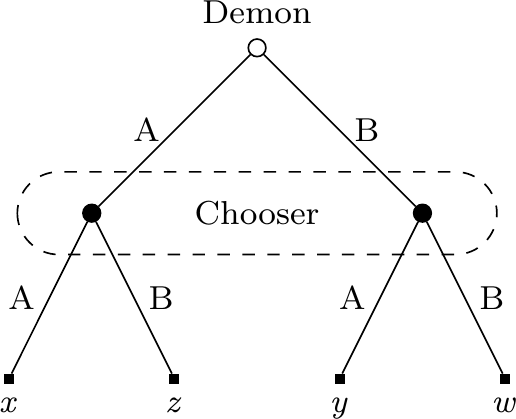
\includegraphics[width=0.5\textwidth,height=\textheight]{intro_files/figure-pdf/fig-gen-dem-problem-text-1.png}

}

\caption{\label{fig-gen-dem-problem-text}Tree Diagram of the generic
demonic decision problem.}

\end{figure}

I've written variables here where the outcomes go. These are going to be
replaced with numbers in any example here. That is, I'll assume that the
value of outcomes can be measured numerically, with greater numbers
being better. I'll come back to this assumption briefly in
Chapter~\ref{sec-ideal}, and more substantively in
Chapter~\ref{sec-expect}.

Following Nozick (\protect\hyperlink{ref-Nozick1969}{1969}), the most
common problem that people discuss involving Demon is what Nozick dubbed
``Newcomb's Problem'', after the physicist who suggested the problem to
him. A Newcomb problem is an instance of
Table~\ref{tbl-gen-dem-problem-text} satisfying the following
constraints.

\begin{itemize}
\tightlist
\item
  \emph{z} \textgreater{} \emph{x}
\item
  \emph{w} \textgreater{} \emph{y}
\item
  \emph{x} \textgreater\textgreater{} \emph{w}
\end{itemize}

The standard example uses (more or less) the values in
Table~\ref{tbl-newcomb}, but all that really matters are the three
inequalities above.

\hypertarget{tbl-newcomb}{}
\begin{longtable}[]{@{}ccc@{}}
\caption{\label{tbl-newcomb}Newcomb's Problem.}\tabularnewline
\toprule\noalign{}
& \textbf{PA} & \textbf{PB} \\
\midrule\noalign{}
\endfirsthead
\toprule\noalign{}
& \textbf{PA} & \textbf{PB} \\
\midrule\noalign{}
\endhead
\bottomrule\noalign{}
\endlastfoot
\textbf{A} & 1000 & 0 \\
\textbf{B} & 1001 & 1 \\
\end{longtable}

Option A and B are typically called `one-boxing' and `two-boxing'
respectively, because they involve selecting either one or two boxes in
the vignette Nozick gives to go along with the story. But what really
matters is the schematic form, not the details of the physical setup.

Nozick distinguishes two approaches to this problem you might take. He
doesn't use the following terms, but they quickly became identified as
Evidential Decision Theory, and Causal Decision Theory. Evidential
Decision Theory (EDT) says that one should first assign values to each
option using the following formulae. I'll just give the formulae for the
case where there are two states of the world, PA and PB, but it should
be clear how to generalise this to the case where there are \emph{m}
possible states. When X is a choice and Y a state, I'll use V(XY) to
mean the value of choosing X in state Y. So for example in
\protect\hyperlink{tbl-newcomb}{Newcomb's Problem}, V(BPA) = 1001; if
Chooser selects B and Demon predicts A, Chooser's payout is 1001. And
I'll use Pr(Y \textbar{} X) to mean the probability of being in state Y
conditional on choosing X. Using this terminology, EDT says that the
value of the choices is:

\begin{longtable}[]{@{}c@{}}
\toprule\noalign{}
\endhead
\bottomrule\noalign{}
\endlastfoot
V(A) = V(APA) · Pr(PA \textbar{} A) + V(APB) · Pr(PB \textbar{} A) \\
V(B) = V(BPA) · Pr(PA \textbar{} B) + V(BPB) · Pr(PB \textbar{} B) \\
\end{longtable}

So in \protect\hyperlink{tbl-newcomb}{Newcomb's Problem}, if Demon is,
say, 90\% reliable, we have:

\begin{longtable}[]{@{}c@{}}
\toprule\noalign{}
\endhead
\bottomrule\noalign{}
\endlastfoot
V(A) = 1000 · 0.9 + 0 · 0.1 = 900 \\
V(B) = 1001 · 0.1 + 1 · 0.9 = 101 \\
\end{longtable}

Then EDT says that higher valued options are better, so A is better than
B, since 900 \textgreater{} 101. And if Demon is even more reliable than
90\%, that gap just grows further.

Causal Decision Theory (CDT), on the other hand, is moved by the
following argument. Whatever Demon has predicted, Chooser is better off
choosing B than A. That, says CDT, settles things; Chooser should take
option B. I think this is right; Chooser should choose B, and they
should do so for this reason. But note that this is not anything like a
complete theory of choice. Two people could agree with this little
argument and have any number of different views about problems that not
so easily disposed of. In this book, especially in
Chapter~\ref{sec-indecisive}, I'll spend a lot of time on problems like
Table~\ref{tbl-stag-decision-first}.

\hypertarget{tbl-stag-decision-first}{}
\begin{longtable}[]{@{}ccc@{}}
\caption[\label{tbl-stag-decision-first}The Stag
Decision.]{\label{tbl-stag-decision-first}The Stag
Decision.\footnote{I say much more about why the problem has this label
  in Appendix~\ref{sec-gad}.}}\tabularnewline
\toprule\noalign{}
& \textbf{PA} & \textbf{PB} \\
\midrule\noalign{}
\endfirsthead
\toprule\noalign{}
& \textbf{PA} & \textbf{PB} \\
\midrule\noalign{}
\endhead
\bottomrule\noalign{}
\endlastfoot
\textbf{A} & 6 & 0 \\
\textbf{B} & 5 & 2 \\
\end{longtable}

It turns out that among people who endorse the little argument for
choosing B in Table~\ref{tbl-newcomb}, there are at least four distinct
views about what to do in
\protect\hyperlink{tbl-stag-decision-first}{Stag Decision}.

\begin{enumerate}
\def\labelenumi{\arabic{enumi}.}
\tightlist
\item
  Frank Arntzenius (\protect\hyperlink{ref-Arntzenius2008}{2008}) and
  Johan E. Gustafsson (\protect\hyperlink{ref-Gustafsson2011}{2011})
  recommend Choosing A.
\item
  Ralph Wedgwood (\protect\hyperlink{ref-Wedgwood2012}{2012}), Dmitri
  Gallow (\protect\hyperlink{ref-Gallow2020}{2020}), Abelard Podgorski
  (\protect\hyperlink{ref-Podgorski2022}{2022}), and David Barnett
  (\protect\hyperlink{ref-Barnett2022}{2022}) recommend choosing B.
\item
  James Joyce (\protect\hyperlink{ref-Joyce2012}{2012}) says that what
  Chooser should do is a function of Chooser's probability distribution
  over their choices prior to deliberating about what to do.
\item
  Jack Spencer (\protect\hyperlink{ref-Spencer2021b}{2021}) and Melissa
  Fusco (\protect\hyperlink{ref-Fuscond}{n.d.}) say that Chooser can
  rationally take either option.
\end{enumerate}

I'm going to side with option 4. Though note that Spencer and Fusco
disagree about what Chooser should do in several other cases. Most
notably, they disagree in cases that are like
\protect\hyperlink{tbl-stag-decision-first}{Stag Decision} but with the
payouts inverted. In those cases, GDT is going to side with Fusco
against Spencer.

It's not obvious, either from the description of the problems or the
history of the philosophical discussion, which if any of these theories
should get the name ``Causal Decision Theory''. Some people write as if
Joyce's view is the unique one that should get that name; indeed many of
the people I've listed above describe themselves as critics of CDT who
are offering an alternative to it. I think that's not the most helpful
way to classify views. All of them accept that in
\protect\hyperlink{tbl-newcomb}{Newcomb's Problem}, Chooser should
choose option B, and that Chooser should choose it because Chooser can't
make a causal difference to whether PA or PB happens, and either way, B
is better than A. That's the core idea behind Causal Decision Theory.

A decision theory should say what to do not just in one problem, but
across a family of problems. It should say what to do in
\protect\hyperlink{tbl-stag-decision-first}{Stag Decision} for example.
As I'm using the term, Causal Decision Theory, as such, is neutral
between the four possible approaches to
\protect\hyperlink{tbl-stag-decision-first}{Stag Decision} So it isn't a
theory. Rather, it is a family of theories, that all agree about what to
do in \protect\hyperlink{tbl-newcomb}{Newcomb's Problem}, and about why
to do it, but disagree in different problems.

So as I'm using the term, Causal Decision Theory is not a theory. That
might be surprising, since it has the word `Theory' in the name. But
we're used to things like the United States of America which includes
parts that are neither States nor in America (e.g., Guam). We can live
with Causal Decision Theory not being a theory, and instead being a
family that agree about what to do, and why to do it, in
\protect\hyperlink{tbl-newcomb}{Newcomb's Problem}. The bulk of this
book will be an in house dispute between causal decision theories,
though I'll spend some time objecting to EDT, and also some time
objecting to other theories that reject both CDT and EDT.\footnote{The
  most notable of these will be the Functional Decision Theory of
  Levinstein and Soares
  (\protect\hyperlink{ref-LevinsteinSoares2020}{2020}), and the
  non-expectationist theories of Quiggin
  (\protect\hyperlink{ref-Quiggin1982}{1982}) and Buchak
  (\protect\hyperlink{ref-BuchakRisk}{2013}).}

\hypertarget{sec-gdt-defined}{%
\section{Gamified Decision Theory}\label{sec-gdt-defined}}

The actual theory I will defend, GDT, is a version of what's sometimes
called causal ratificationism.

The `causal' in causal ratificationism means that there are constraints
on the proper formulation of a decision problem. EDT says it does not
matter how we divide the world into states; decision theory should give
the same verdict. If we rewrite
\protect\hyperlink{tbl-newcomb}{Newcomb's Problem} with the states being
that Demon predicted correctly, and that Demon predicted incorrectly,
EDT gives the same recommendation, for essentially the same reason. GDT,
like all causal theories, rejects this. The correct formulation of a
decision problem requires that the states, like PA and PB, be causally
independent of the choices that Chooser makes. I have a fairly strong
version of this independence constraint, which I'll discuss more in
Chapter~\ref{sec-causal}.

The `ratificationism' in causal ratificationism means that Chooser will
ratify their choice once they make it, i.e., that Chooser will not
regret a rational choice as soon as it is made. Formally, this means
that Chooser will only choose A in cases like
Table~\ref{tbl-gen-dem-problem-text} if the following inequality
holds.\footnote{In general, the sum on each side of the inequality
  ranges over all possible states, so if there are more than two states,
  there will be more than two summands on either side. And A must be
  ratified compared to all alternatives, so if there are more than two
  options, this inequality must hold if you replace B with C, D, or any
  other choice.}

\begin{longtable}[]{@{}
  >{\centering\arraybackslash}p{(\columnwidth - 0\tabcolsep) * \real{1.0000}}@{}}
\toprule\noalign{}
\endhead
\bottomrule\noalign{}
\endlastfoot
V(APA) · Pr\textsubscript{A}(PA) + V(APB) · Pr\textsubscript{A}(PB) ≥
V(BPA) · Pr\textsubscript{A}(PA) + V(BPB) · Pr\textsubscript{A}(PB) \\
\end{longtable}

By Pr\textsubscript{A} I mean the rational probabilities that Chooser
has after choosing A. If there is more than one rational probability
that Chooser could have, all that matters is that the inequality hold
for one such probability function.\footnote{If there is more than one
  alternative to A, and more than one rational probability function, the
  rule is that there is some probability function such that A does
  better than every possible alternative, if we put that function into
  the inequality above. It's not enough that for each alternative there
  is some probability function that judges A to be better than the
  alternative.} In somewhat technical English, what this inequality says
is that once A is chosen, the expected value of choosing A is at least
as great as the expected value of having chosen B. That's what I mean by
ratifiability; once Chooser selects A, they think it was for the best
(or at least equal best) that they chose it.

I'm far from the first to endorse ratifiability as a constraint on
decisions. It's defended by William Harper
(\protect\hyperlink{ref-Harper1986}{1986}), in a paper that was a
central inspiration for this project, both because of its conclusions,
and because of the way it connected decision theory to game theory. I'll
talk about the ratifiability constraint much more in
Chapter~\ref{sec-ratify}.

GDT, as I'm defining it, has three extra features beyond this causal
ratification constraint, and I'll end this chapter with a brief
discussion of each of them.

GDT says that permissible choices are not weakly dominated. An option
weakly dominates another if it could be better, and couldn't be worse.
So in Table~\ref{tbl-weak-dominance-example}, A is not a permissible
choice because it is weakly dominated by B.

\hypertarget{tbl-weak-dominance-example}{}
\begin{longtable}[]{@{}ccc@{}}
\caption{\label{tbl-weak-dominance-example}An example of weak
dominance.}\tabularnewline
\toprule\noalign{}
& \textbf{PA} & \textbf{PB} \\
\midrule\noalign{}
\endfirsthead
\toprule\noalign{}
& \textbf{PA} & \textbf{PB} \\
\midrule\noalign{}
\endhead
\bottomrule\noalign{}
\endlastfoot
\textbf{A} & 2 & 0 \\
\textbf{B} & 2 & 1 \\
\end{longtable}

Since B could be better than A, if Demon predicted B, and could not be
worse than A, at worst they produce the same outcome if Demon predicts
A, B weakly dominates A. And weakly dominated actions are not rational
choices. So in this problem the only rational choice is B. This is not
particularly intuitive, but I don't think agreement with first pass
intuition is a particularly strong constraint on decision theories, for
reasons I'll go over in Chapter~\ref{sec-expect}. And I'll have much
more to say about weak dominance, and in particular why I reject an
iterated version of the weak dominance constraint, in
Chapter~\ref{sec-weak}.

In dynamic choices, GDT says that Chooser must satisfy two constraints.
First, the plan they make for what to do over time, what we'll call a
strategy\footnote{A strategy in this sense must plan for what to do in
  every possibility, including possible choices ruled out by earlier
  choices.}, must be a permissible choice of strategy. Second, at each
point in time, they must choose an option that would be permissible were
the dynamic choice problem to have started at that point, with that set
of options. These two constraints, which I'll discuss much more in
chapter Chapter~\ref{sec-dual}, have some surprising consequences.
Imagine that Chooser has the following two-stage problem. At stage 1,
they can choose to Exit or Continue. If they Exit, they get 5. If they
continue, they make a choice in the problem depicted in
Table~\ref{tbl-first-dynamic-example}.\footnote{In this problem, the
  Demon makes a prediction after Chooser opts to Continue, but this
  prediction is only revealed after Chooser selects A or B.}

\hypertarget{tbl-first-dynamic-example}{}
\begin{longtable}[]{@{}ccc@{}}
\caption{\label{tbl-first-dynamic-example}The second stage of a dynamic
problem.}\tabularnewline
\toprule\noalign{}
& \textbf{PA} & \textbf{PB} \\
\midrule\noalign{}
\endfirsthead
\toprule\noalign{}
& \textbf{PA} & \textbf{PB} \\
\midrule\noalign{}
\endhead
\bottomrule\noalign{}
\endlastfoot
\textbf{A} & 4 & 4 \\
\textbf{B} & 0 & 8 \\
\end{longtable}

The plan of Continuing, then choosing A, is not a sensible plan. Chooser
knows from the start that there is a plan which is guaranteed to be
better, namely Exiting. If they Exit, they are guaranteed to get 5, if
they Continue then choose A, they are guaranteed to get 4. So they may
not Continue then choose A. But this does not mean that they must Exit.
They may Continue and choose B. Now here's the surprising part. If they
faced Table~\ref{tbl-first-dynamic-example} as the first choice they
have to make, they could choose B, but they also could choose A. In
Table~\ref{tbl-first-dynamic-example}, A is ratifiable and not weakly
dominated. So GDT is not a purely consequentialist decision theory. By
that I mean that sometimes, choices that Chooser makes earlier in a
dynamic choice situation constrain which choices are rational later in
the game. A lot of versions of CDT do not specify how they are to be
extended into theories of dynamic choice, but my impression is that many
philosophers, and especially many philosophers who endorse CDT, do think
decision theory should be purely consequentialist, and GDT disagrees
with them on this point.

There are some decision theorists who agree with GDT that decisions
should not be strictly consequentialist. These include the resolute
theorists, in the sense of McClennan
(\protect\hyperlink{ref-McClennan1990}{1990a}), and the functional
theorists, in the sense of Levinstein and Soares
(\protect\hyperlink{ref-LevinsteinSoares2020}{2020}). But GDT disagrees
with them as well. Those theorists think that the only thing Chooser
must do is choose a sensible plan, and then at each stage Chooser should
just carry it out. In section Section~\ref{sec-against-equivalence} I'll
argue against the idea that the choice of a rational strategy always
lines up with the choice of rational moves at each point in a dynamic
choice problem.\footnote{One might have expected it would be easy to
  generate examples where this fails in GDT, by simply translating the
  examples of games involving incredible threats
  (\protect\hyperlink{ref-Bonanno2018}{Bonanno 2018, 86}) into demonic
  decision problems. It turns out to be harder than one might have
  expected, or at least than I originally expected, to come up with such
  a case where (a) one player is Demon, and (b) the `threat' strategy is
  not weakly dominated. And in Chapter~\ref{sec-weak} I'm going to
  follow Stalnaker (\protect\hyperlink{ref-Stalnaker1999}{1999}) in
  ruling out weakly dominated strategies. That explains some of the
  complications in the example to follow.} Then in section
Section~\ref{sec-against-pure-strategy} I'll argue against the view that
choosing a rational strategy suffices for rational play in a dynamic
choice problem. The upshot will be that GDT requires that every action
be sensible at the time it is taken, not just part of a sensible
strategy, and that conflicts with most other theories that care about
strategies.

Finally, my version of GDT says that what matters for rational choice is
what probabilities over states are rational, not which probabilities
Chooser happens to endorse. GDT is a theory of rational choice
simpliciter, not a theory of rational choice given possibly irrational
beliefs. I'll have more to say about this in
Chapter~\ref{sec-substantive}.

\hypertarget{sec-dynamic-argue}{%
\section{Dynamic Arguments for Static
Theories}\label{sec-dynamic-argue}}

The full argument for GDT takes the bulk of the book to set out. There
is, however, a much shorter argument for something in the ballpark of
GDT, and certainly for something distinct from most existing views in
the philosophical literature, that starts with three principles about
dynamic choice. This is not because GDT is itself a dynamic theory; in
the first instance it is a version of causal ratificationism, a static
theory. The point is that only certain static theories are even capable
of being extended into decent theories of dynamic choice, and this is a
tighter constraint than has always been appreciated.

The first of the three principles concerns the following
situation.\footnote{In Chapter~\ref{sec-indecisive} I'm going to call
  this the Single Choice Principle, because it concerns dynamic choice
  situations where Chooser has only one possible choice to make.} If
\emph{p} is false, Chooser's payouts are (causally) independent of
anything they do. If \emph{p} is true, Chooser will have to make a
single choice. But if they do, they won't learn anything relevant other
than that \emph{p} is true before choosing. In game theoretic terms, the
tree of the game Chooser is playing has just one node where they act,
and it's a singleton information set. These are fairly tight
constraints; most dynamic choice situations involve either multiple
possible choices, or multiple things that one could learn before a
choice. We're just interested in this very special case.

The principle I rely on is that in such a situation, it doesn't matter
whether Chooser is asked to choose before or after learning that
\emph{p} is true. That is, if they are asked to come up with a strategy,
which in this case is just a plan for what to do if \emph{p} is true,
that's just the same as being told that \emph{p} is true, and being
asked to come up with a move. Slightly more informally, the following
two questions should get the same answer because in some deep sense they
are the same question:

\begin{enumerate}
\def\labelenumi{\arabic{enumi}.}
\tightlist
\item
  If \emph{p} is true, what do you want to do?
\item
  Hey, \emph{p} is true. What do you want to do?
\end{enumerate}

This principle is violated by, among others, the theory of choice that
Lara Buchak (\protect\hyperlink{ref-BuchakRisk}{2013})
defends.\footnote{Buchak offers a very clear outline of her view in her
  (\protect\hyperlink{ref-Buchak2017}{2017}).} Imagine that Suzy has two
things she is planning to give away. The first is a lottery ticket that
has a 50\% chance of being worth \$4, and a 50\% chance of being worth
nothing. The second is a dollar. She is going to give one to Billy and
the other to Teddy. She comes up with the following somewhat convoluted
plan to decide what to do. She's going to flip a fair coin. If it lands
heads, Billy will get the ticket. If it lands tails, Billy will get a
choice of the ticket or the dollar. Billy's risk-function\footnote{On
  the role of risk-functions in Buchak's theory, see
  (\protect\hyperlink{ref-Buchak2017}{Buchak 2017, 2366}).} \emph{r} is
\emph{r}(\emph{p})~=~\emph{p}\textsuperscript{2}. And money has an
ever-so-slightly declining marginal utility for Billy.\footnote{The
  example is not sensitive to the details on this point, but to make it
  concrete, imagine that Billy's utility from wealth \emph{w} is
  log(\emph{w}), and he currently has a few thousand dollars.} Then if
Billy follows Buchak's theory, he'll say the following things. Ask him
before the coin is flipped what he would like if it lands tails, and
he'll say the ticket. Tell him the coin has landed tails, and ask him
what he'd like, and he'll say the dollar. That looks inconsistent, even
incoherent, to me, and it's enough reason for me to look for a separate
theory.\footnote{In Appendix~\ref{sec-buchak} I go over a more general
  version of this example, showing that unless the risk-function is the
  identity function, such a problem can arise. If the risk-function is
  the identity function, Buchak's theory does not disagree with GDT.}

The second principle says that in a dynamic choice situation, every
choice that a rational chooser makes must make sense in purely
forward-looking terms. That is to say, every choice must be one that
could be rationally made if it were the first choice being made in a
different, simpler, dynamic choice. It's easiest to see what this rules
out by looking at an example. This is going to be a version of
\protect\hyperlink{tbl-newcomb}{Newcomb's Problem} without any suspense,
i.e., with the Chooser being allowed to look inside the boxes.

Chooser is going to be presented with two boxes, one red and one blue.
The boxes will be open, so Chooser will see what's in them. Chooser will
be allowed to take the contents of one of them, at their choice. There
is a Demon who predicted Chooser's choice. If Demon predicted Chooser
would choose the red box, they put \$10 in the red box, and \$11 in the
blue box. If Demon predicted Chooser would choose the blue box, they put
\$0 in the red box, and \$1 in the blue box. The second principle says
that in this case, Chooser must take the blue box. What it rules out is
the following reasoning, which is endorsed by, e.g., Levinstein and
Soares (\protect\hyperlink{ref-LevinsteinSoares2020}{2020}). The optimal
strategy is to plan to take the red box, since on average that gets \$10
rather than \$1. Then when the boxes are opened, what Chooser should do
is carry out the optimal strategy, i.e., take the red box. The second
principle says that reasoning is illegitimate. If Chooser is going to
take the red box now, they must be capable of defending that decision
using purely forward-looking considerations.\footnote{This is consistent
  with what I said about about GDT not being a purely consequentialist
  theory. There I said that non-consequentialist constraints can rule
  out something makes sense on purely consequentialist grounds. Here I'm
  saying that only things that are allowed by consequentialism are
  allowed full stop.} And that's impossible to do, since there is quite
clearly one more dollar in the blue box. The only consideration in
favour of the red box is backward-looking; it correlates with getting a
more favourable distribution of funds to the boxes.

The third principle is a converse of sorts to the third. It says that at
the end of a series of choices, a rational chooser must be able to
defend why they made that series of choices rather than some alternative
series.\footnote{There are a bunch of caveats needed on this, and I go
  over them more in Chapter~\ref{sec-dual}. For now, all that matters is
  that the example I'll use does not violate any of the needed caveats.}
To see why this matters, it helps to use a version of GDT that I used to
believe was correct, before I considered what it said about examples
like Table~\ref{tbl-first-dynamic-example}. This theory says that all
that matters for choice at a time is that one do something ratifiable
(and not weakly dominated), and that all that matters for dynamic choice
is that one equates the possibility of reaching a future choice with a
lottery ticket whose payouts are the payouts of that later choice, with
the probabilities of each payout of the ticket the same as the
probability one gives to the payouts of the later choice.

Start with this theory, and think about the following kind of Chooser.
They think that if they don't exit, and instead choose to play
Table~\ref{tbl-first-dynamic-example}, it's just as likely that they'll
choose A as B. After all, both are rational. So playing the game has an
expected return of 6, while exiting has a guaranteed return of 5, so
they play the game. And then they play A, and they get 4. This seems
irrational; they could have got 5. The third principle says that it is
irrational. The strategy, play the game then choose A, is not a strategy
one could defend as a whole. The alternative strategy of
exiting\footnote{To be more precise, there are multiple exit strategies,
  which differ in what one is disposed to do if one doesn't exit. This
  level of precision will occasionally matter, but not that often.}
strictly dominates it. According to GDT, a series of choices, each
rational in themselves, can be collectively irrational. And that's what
is distinctive about the third principle. In game-theoretic terms, it
says that one's sequence of choices (and dispositions to choose in
unreached nodes of the game-tree) must be defensible if one was choosing
a strategy. And this turns out to be a non-trivial constraint.

None of these three principles will strike people working in decision
theory as particularly novel. I've framed them in terms of
choice-worthiness rather than preference, which makes them a bit weaker
and hence more plausible. And as the book goes on I'll offer some
somewhat new arguments for them. But none of them alone are particularly
innovative. What is, I think, more innovative, is putting them together.
While many theories exist that satisfy at least one of them, or even
satisfy some pair of them, as far as I can tell, only versions of causal
ratificationism look capable of satisfying all three.

If there is a single master argument of the book, it is that the right
decision theory complies with these three principles, only causal
ratificationism complies with these three principles, so the correct
decision theory is a form of causal ratificationism. I'll have much more
to say about the principles, and about the particular form of causal
ratificationism I prefer. That argument, however, is the simplest guide
to where we're going.

\bookmarksetup{startatroot}

\hypertarget{sec-ideal}{%
\chapter{Idealised}\label{sec-ideal}}

\hypertarget{sec-ideal-intro}{%
\section{Introducing Ideal Theory}\label{sec-ideal-intro}}

Game theorists, like philosophical decision theorists, are doing ideal
theory. To see that they are doing ideal theory, compare what they say
about two problems: Salesman and Basketball. The first is a version of
what Julia Robinson dubbed the `travelling salesman' problem.\footnote{The
  dubbing is in Robinson (\protect\hyperlink{ref-Robinson1949}{1949}).
  For a thorough history of the problem, see Schrijver
  (\protect\hyperlink{ref-Schrijver2005}{2005}). For an accessible
  history of the problem, which includes these references, see the
  wikipedia page on `Traveling Salesman Problem'.}

\begin{quote}
\textbf{Salesman} Chooser is given the straight line distance between
each pair of cities from the 257 represented on the map in
Figure~\ref{fig-salesman-points}. Using this information, Chooser has to
find as short a path as possible that goes through all 257 cities and
returns to the first one. The longer a path Chooser selects, the worse
things will be for Chooser.
\end{quote}

\begin{figure}

{\centering 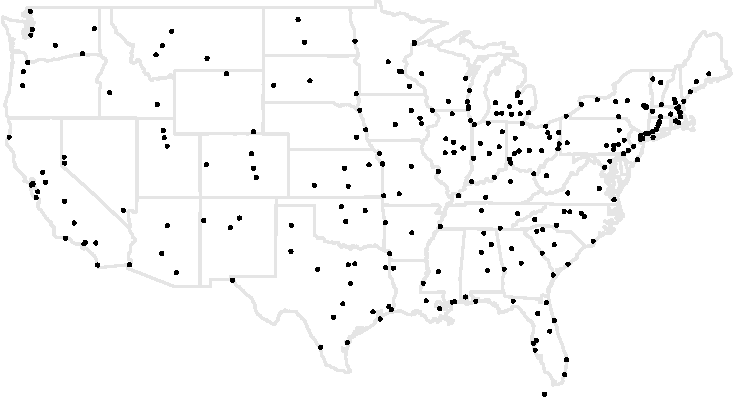
\includegraphics{idealised_files/figure-pdf/fig-salesman-points-1.pdf}

}

\caption{\label{fig-salesman-points}The 257 cities that must be visited
in the Salesman problem.}

\end{figure}

Since there are 256! possible paths, and 256! ≈ 10\textsuperscript{727},
Chooser has a few options here.\footnote{The 256 cities are the cities
  in the lower 48 states from the 312 cities in North America that John
  Burkardt mapped in his dataset Cities, available at
  \href{https://people.sc.fsu.edu/~jburkardt/datasets/cities/cities.html}{people.sc.fsu.edu/\textasciitilde jburkardt/datasets/cities/cities.html}.}
Game theorists, and philosophical decision theorists, start with the
assumption that the people in their models can solve these problems in
zero time and at zero cost. Or, at the very least, that the people can
emulate someone who solves these problems in zero time and at zero cost.
That's not even approximately true for any actual person without
technological assistance. Even with knowledge of the problem and a good
computer, there are not that many actual people who you could properly
model as being able to solve it in zero time and at zero cost.

The question of how to think about people who do have to spend time and
resources to solve a problem like this is an interesting one. We might
call that problem one in \emph{non-ideal decision theory}.\footnote{I'm
  borrowing the term `non-ideal' from work in political philosophy. See
  Valentini (\protect\hyperlink{ref-Valentini2012}{2012}) for a good
  survey of some relevant work, and Mills
  (\protect\hyperlink{ref-Mills2005}{2005}) for an important critique of
  the centrality of ideal theory in political philosophy. Critics of
  ideal theory, such as Mills, and Sen
  (\protect\hyperlink{ref-Sen2006}{2006}), argue that we shouldn't base
  non-ideal theory on ideal theory. I'm going to agree, but my focus is
  primarily in the other direction. I'm going to argue that it isn't a
  constraint on ideal theory that it is useful in constructing a
  non-ideal theory.} I won't say much about non-ideal decision theory in
the body of this book, though I'll come back to it in
Appendix~\ref{sec-nidt}. What I mostly want to do now is use Salesman to
say something about what the difference between ideal and non-ideal
theory is. And that difference is brought up vividly by the following
problem.

\begin{quote}
\textbf{Basketball} Chooser is at a casino, and a basketball game is
about to start. Chooser knows that basketball games don't have draws or
ties; one side will win. And Chooser knows the teams are equally
balanced; each team is 50\% likely to win. Chooser has three options.
They can bet on the Home team to win, bet on the Away team to win, or
Pass, and not bet. If they bet, they win \$100 if the team they bet on
wins, and lose \$110 if that team loses. If they Pass, they neither gain
nor lose anything.
\end{quote}

Ideal decision theory says that in Basketball, Chooser should Pass.
That's not the optimal outcome for Chooser. The optimal outcome is that
they bet on the winning team. But since they don't know who that is, and
either bet will, on average, lose them money, they should Pass rather
than bet on Home or Away. We could have a theory that just evaluated the
possible outcomes in any decision. I'll call this Outcome Evaluation
Theory. Contrast this with two other theories. Game theory says that the
ideal agent chooses the shortest route, whatever it is, in Salesman and
does not bet in Basketball. If an ordinary reasonable person was
advising a friend facing these two problems, they would give the same
advice as the game theorist about Basketball, but in Salesman they would
not simply say \emph{Choose the shortest path!}, since that's useless
advice. Rather they would suggest something about how to solve the
problem, possibly by looking up strategies.

So we have three theories on the table: Outcome Evaluation Theory; the
game theory approach, which I'll call Ideal Decision Theory; and the
ordinary reasonable person approach, which I'll call Non-Ideal Decision
Theory. We can distinguish these three theories by what they say to do
in two examples introduced so far: Salesman and Basketball.

\hypertarget{tbl-three-theories}{}
\begin{longtable}[]{@{}ccc@{}}
\caption{\label{tbl-three-theories}How three kinds of theories handle
two problems.}\tabularnewline
\toprule\noalign{}
\textbf{Theory} & \textbf{Salesman} & \textbf{Basketball} \\
\midrule\noalign{}
\endfirsthead
\toprule\noalign{}
\textbf{Theory} & \textbf{Salesman} & \textbf{Basketball} \\
\midrule\noalign{}
\endhead
\bottomrule\noalign{}
\endlastfoot
Outcome Evaluation & Shortest route & Bet on winner \\
Ideal Decision & Shortest route & Pass \\
Non-Ideal Decision & Study optimization & Pass \\
\end{longtable}

Game theory agrees with the middle row. GDT, the theory I'm developing
in this book, does so too. And so do almost all decision theorists
working in philosophy.\footnote{The exceptions are people working in
  `descriptive decision theory'
  (\protect\hyperlink{ref-ChandlerSEP}{Chandler 2017}). But that's
  normally not taken to be a normative theory in any respect; it isn't
  about what people should do in problems like Salesman, but what they
  actually do.} So in trying to convince philosophers to adopt GDT, I'm
not asking them to change their view on this point. But still, this is
odd. What is the benefit of a theory of decision that does not produce
the best outcomes, and does not produce useful, reasonable advice?

We could say that if Chooser were ideal, they would agree with Ideal
Decision Theory.\footnote{This claim isn't obvious. Why should being
  ideal require computational perfection, but not informational
  perfection? I'll have more to say about this in
  Section~\ref{sec-why-this-ideal}.} But why we should care about what
would have if Chooser were ideal, since Chooser is not in fact ideal?
One might think that knowing what the ideal is gives Chooser something
to aim for. Even if Chooser is not ideal, they can try to be closer to
the ideal. The problem is that trying to be more like the ideal will
make things worse. The ideal agent will announce the best answer they
have after spending no time calculating the solution to Salesman, and
resembling the ideal agent in that respect will make Chooser
worse.\footnote{This is a special case of Lipsey and Lancaster's Theory
  of the Second Best (\protect\hyperlink{ref-LipseyLancaster}{Lipsey and
  Lancaster 1956}). If you don't have control over every parameter,
  setting the parameters you do control to the ideal values is generally
  inadvisable.} And there is a separate problem. Why say it is ideal to
make a choice in Basketball that Chooser knows will lead to a
sub-optimal outcome? We can make progress on both these problems, what
it means to say something is ideal, and why we should care about the
ideal, but stepping back and asking what we even mean by `ideal', and
`idealisation'.

In philosophy, it turns out we have two very different uses of the term
`idealisation'. One is the kind of idealisation we see in, for example,
Ideal Observer theories in ethics. The other is the kind of idealisation
we see in, for example, Ideal Gas models in chemistry. It's important to
not confuse the two. Think about the volumeless, infinitely dense,
molecules in an Ideal Gas model. To say that this is an idealised model
is not to say that having volume, taking up space, is an imperfection.
The point is not to tell molecules what the perfect size is. (``The only
good molecule is a volumeless molecule.'') Nor is it to tell them that
they should approximate the ideal. (``Smaller the better, fellas.'')
It's to say that for some predictive and explanatory purposes, molecules
behave no differently to how they would behave if they took up no
space.\footnote{I'm drawing here on work on the nature of idealisations
  by Michael Strevens (\protect\hyperlink{ref-Strevens2008}{2008}) and
  by Kevin Davey (\protect\hyperlink{ref-Davey2011}{2011}).}

The best way to understand game theorists, and most philosophical
decision theorists, is that they are using idealisations in this latter
sense. The ideal choosers of decision theory are not like the Ideal
Observers in ethics, but like the Ideal Gases. The point of the theory
is to say how things go in a simplified version of the case, and then
argue that this is useful for predictive and explanatory purposes
because, at least some of the time, the simplifications don't make a
difference.

\hypertarget{sec-uses-ideal}{%
\section{Uses of Ideal Theory}\label{sec-uses-ideal}}

Still, this approach raises two pressing questions. One is why we should
be interested in a model that is so idealised. The other is why we don't
idealise even further, idealising away from informational limitations as
well as computational ones.\footnote{John Conlisk
  (\protect\hyperlink{ref-Conlisk1996}{1996}) stresses that explaining
  the asymmetry here is a big part of the challenge. That paper had a
  big influence in how I'm thinking about the problem, and several of
  the citations below are from it.}

All social sciences use idealised models of some kind or other. The fact
that real humans can't solve problems like Salesman, but the modelled
humans can, isn't in itself a problem. Modelled humans are always
different in some respects to real humans. It is only a problem if the
differences matter. For example, if you are trying to model when humans
fail at maximisation problems, don't use a model that idealises away
from computational limitations.

The real challenge is that some idealisations are useless. If all we end
up saying is that when it's more likely to rain, more people take
umbrellas, we don't need books full of math to say that. Here's how
Keynes puts the complaint, in a closely related context.

\begin{quote}
But this \emph{long run} is a misleading guide to current affairs.
\emph{In the long run we are all dead}. Economists set themselves too
easy, too useless a task if in tempestuous seasons they can only tell us
that when the storm is long past the ocean will be flat again.
(\protect\hyperlink{ref-Keynes1923}{Keynes 1923, 80}, emphasis in
original)
\end{quote}

Don't focus on the temporal connotations of Keynes's terminology of
`long run'. What's characteristic of his long run is not that it takes
place in the distant future. What is characteristic of it instead is
that it takes place in a world where some sources of interference are
absent. It's a world where we sail but there are no storms. It's a study
where we abstract away from storms and other unfortunate complications.
And that's what's characteristic of Ideal Decision Theory. We know that
people cannot easily solve hard arithmetic problems, but we abstract
away from that fact. Does this leave the resulting theory ``easy and
useless''?

To see that it's not ``easy'', it simply suffices to take a casual
glance at any economics journal. But what about Keynes's suggestion that
it is ``useless''? It turns out there are some surprising results that
we need the details of something like GDT to generate. One nice case of
this is the discussion of Gulf of Mexico oil leases in Wilson
(\protect\hyperlink{ref-Wilson1967}{1967}).\footnote{I learned about
  this paper from the excellent discussion of the case in Sutton
  (\protect\hyperlink{ref-Sutton2000}{2000}).} Another example of this
working is George Akerlof's discussion of the used car market Akerlof
(\protect\hyperlink{ref-Akerlof1970}{1970}). In the twentieth century,
it was common for lightly used cars to sell at a massive discount to new
cars. There was no good explanation for this, and it was often put down
to a brute preference for new cars. What Akerlof showed was that a model
where (a) new cars varied substantially in quality, and (b) in the used
car market, buyers had less information about the car than sellers, you
could get a discount similar to what you saw in real life even if the
buyers had no special preference for new cars. Rather, buyers had a
preference for good cars, and took the fact that a car was for resale
within months of being first bought to be evidence that it was badly
made. It was important for Akerlof's explanatory purposes that he could
show that people were being rational, and this required that he have a
decision theory that they followed. In fact what he used was something
like GDT. We now have excellent evidence that something like his model
was correct. As the variation in quality of new cars has declined, and
the information available to buyers of used cars has risen, the used car
discount has just about vanished. (In fact it went negative during the
COVID-19 pandemic, for reasons I don't at all understand.)

Here's an even simpler surprising prediction that you need something
like GDT to get, and which is relevant to some debates in philosophical
decision theory.\footnote{Bonanno
  (\protect\hyperlink{ref-Bonanno2018}{2018, 216}) makes a somewhat
  similar point with the example of the drowning dog.} Imagine Row and
Column are playing rock-paper-scissors. A bystander, C, says that he
really likes seeing rock beat scissors, so he will pay whoever wins by
playing rock \$1. Assuming that Row and Column have no ability to
collude, the effect of this will to add \emph{c} to the value of playing
Rock against Scissors, where \emph{c} is the value of the dollar
compared to the value of winning the game. This changes the game they
are playing from Table~\ref{tbl-rps-basic} to
Table~\ref{tbl-rps-modified}.

\begin{table}

\caption{\label{tbl-rps}Two versions of
Rock-Paper-Scissors}\begin{minipage}[t]{0.50\linewidth}
\subcaption{\label{tbl-rps-basic}Original game}

{\centering 

\begin{tabular}[t]{cccc}
\toprule
 & \textbf{Rock} & \textbf{Paper} & \textbf{Scissors}\\
\textbf{Rock} & 0,0 & -1,1 & 1,-1\\
\textbf{Paper} & 1,-1 & 0,0 & -1,1\\
\textbf{Scissors} & -1,1 & 1,-1 & 0,0\\
\bottomrule
\end{tabular}

}

\end{minipage}%
%
\begin{minipage}[t]{0.50\linewidth}
\subcaption{\label{tbl-rps-modified}Modified game}

{\centering 

\begin{tabular}[t]{cccc}
\toprule
 & \textbf{Rock} & \textbf{Paper} & \textbf{Scissors}\\
\textbf{Rock} & 0,0 & -1,1 & 1+\emph{c},-1\\
\textbf{Paper} & 1,-1 & 0,0 & -1,1\\
\textbf{Scissors} & -1,1+\emph{c} & 1,-1 & 0,0\\
\bottomrule
\end{tabular}

}

\end{minipage}%

\end{table}

The surprising prediction is that this will \emph{decrease} the
frequency with which the bystander gets their way. The incentive will
not make either party play rock more often, they will still play it one
third of the time, but the frequency of scissors will decrease, so the
\emph{rock smash} outcome will be less frequent. Moreover, the bigger
the incentive, the larger this increase will be\footnote{The proof is in
  Appendix~\ref{sec-rps}.}. Simple rules like ``When behaviour is
rewarded, it happens more often'' don't always work in strategic
settings, and it takes some care to tell when they do work.

The point of decision theory is not to advise people on what to do in
Rock-Paper-Scissors, or in Salesman. In each case, it would give bad
advice. Really you should try to read your opponent's body shape for
clues in Rock-Paper-Scissors, and find some good software in Salesman.
You won't find either of those bits of advice in a game theory, or
decision theory, text. Rather, the point is be part of explanations like
why there was such a large discount on used cars in the 20th century,
and why the bystander's gambit won't work in my modified version of
Rock-Paper-Scissors. David Lewis gives a similar account of the purpose
of decision theory in a letter to Hugh Mellor. The context of the
letter, like the context of this section, is a discussion of why
idealisations are useful in decision theory. Lewis writes,

\begin{quote}
We're describing (one aspect of) what an ideally rational agent would
do, and remarking that somehow we manage to approximate this, and
perhaps -- I'd play this down -- advising people to approximate it a bit
better if they can. (\protect\hyperlink{ref-Lewis1981Mellor}{Lewis
2020a, 432})
\end{quote}

\hypertarget{sec-why-this-ideal}{%
\section{Why This Idealisation}\label{sec-why-this-ideal}}

Still, there are a lot of ways to idealise away from the details of
individual humans. Why do we delete the differences from rationality,
and not the differences from full-informedness, or the differences from
something that lacks normative significance? One simple answer is that
people have used this idealisation and it has (to some extent) worked.
But there is a little more to say.

Take some generalisation about human choosers that isn't particularly
rational, is true in most but not all cases, and which it would simplify
our description of various cases to say it holds in all cases. Why don't
we use the idealisation that says it does in fact hold in all cases? The
answer here depends a bit on the `we'. Some generalisations about less
than ideally rational behavior are useful in empirical studies of
consumer choice.\footnote{See
  (\protect\hyperlink{ref-Barta2023}{\textbf{Barta2023?}}) for a
  relatively recent example, picked more or less at random.} But there
is a reason that philosophers and more theoretical economists have
focussed on rational idealisations. The thought is that a lot of
deviations from rationality are short-cuts that are sensible to use when
the stakes are low. But in high-stakes situations, humans will more
closely approximate ideally rational agents. (This might be coupled with
the suggestion that over time they will do this better, simply because
the ones who more closely approximate the rational choice will increase
their market share.) And getting correct predictions and explanations in
high-stakes cases might be particularly important in understanding
society and the economy. So while non-rational idealisations might be
crucially important in understanding store design (e.g., why
supermarkets have produce at the entrance), rational idealisations are
needed for understanding the nature of stock markets and business
investment.

That reasoning looks like it might over-generate. In high-stakes cases,
people are not only more careful with their decision making process,
they are more careful about acquiring information before they decide. If
our focus is high-stakes decision making, and I think it has to be to
motivate rational idealisations, why don't we also abstract away from
informational limitations of the deciders? After all, the decider will
try to remove those limitations before deciding in these high-stakes
cases. The answer is that in some cases, and these are the cases that
decision theory is most useful in explaining, there are in principle
reasons why the decider can't do anything about certain informational
limitations. The information might be a fact about the result of a
chance-like process that is unknowable either in principle, or in any
practical way. Or there might be someone else who has just as much
incentive to keep the information hidden as the decider has to seek it
out. The latter is what happens when someone is selling a lemon, for
example. I don't have anything like a proof of this, but I suspect that
most uses of game theory or decision theory to explain real-world
phenomena will fall into one or other of these categories: there are
relevant facts that the decider can't know, either because they have to
decide before decisive evidence is revealed, or because someone just as
well resourced as them is determined to prevent them getting the
information.

\hypertarget{sec-ideal-bonus}{%
\section{Two Bonus Uses}\label{sec-ideal-bonus}}

There are two other advantages to using the particular idealisation that
game theorists and decision theorists have settled on, i.e., idealise
away from computational but not informational limitations. The first can
be seen from this famous quote from Frank Knight, an early proponent of
the view of idealisations in decision theory that I'm endorsing here.

\begin{quote}
It is evident that the rational thing to do is to be irrational, where
deliberation and estimation cost more than they are worth. That this is
very often true, and that men still oftener (perhaps) behave as if it
were, does not vitiate economic reasoning to the extent that might be
supposed. For these irrationalities (whether rational or irrational!)
tend to offset each other. The applicability of the general ``theory''
of conduct to a particular individual in a particular case is likely to
give results bordering on the grotesque, but \emph{en masse} and in the
long run it is not so. The \emph{market} behaves \emph{as if} men were
wont to calculate with the utmost precision in making their choices. We
live largely, of necessity, by rule and blindly; but the results
approximate rationality fairly well on an average.
(\protect\hyperlink{ref-Knight1921}{Knight 1921, 67n1})
\end{quote}

I don't agree with everything Knight says here; I think he's much too
quick to assume that deviations from rationality will
``offset''.\footnote{See Conlisk
  (\protect\hyperlink{ref-Conlisk1996}{1996}) for many, many examples
  from both theory and practice where they do not.} But that's something
to be worked out on a case-by-case basis. We should not presuppose in
advance either that the imperfections be irrelevant or that they will be
decisive.

Despite that, I quoted Knight here because there is an important point
to I do agree with. If we don't act by first drawing Marshallian curves
and solving optimisation problems, how do we act? As Knight says, we
typically act ``by rule''. Our lives are governed, on day-by-day,
minute-by-minute basis, by a series of rules we have internalised for
how to act in various situations. The rules will typically have some
kind of hierarchical structure - do this in this situation unless a
particular exception arises, in which case do this other thing, unless
of course a further exception arises, in which case, and so on. And the
benefit of adopting rules with this structure is that they, typically,
produce a good trade off between results and cognitive effort.

One useful role for idealised decision theory is in the testing and
generation of these rules. We don't expect people who have to make
split-second decisions to calculate expected utilities. But we can
expect them to learn some simple heuristics, and we can expect theorists
to use ideal decision theory to test whether those heuristics are right,
or whether some other simple heuristic would be better. This kind of
approach is very useful in sports, where athletes have to make decisions
very fast, and there is enough repetition for theorists to calculate
expected utilities with some precision. But it can be used in other
parts of life, and it is a useful role for idealised decision theory
alongside its roles in prediction and explanation.

The other benefit of idealised decision theory is that it has turned out
to be theoretically fruitful. This has included fruits that I, at least,
would never have expected. It turns out that sometimes one gets a
powerful kind of explanation from very carefully working out the ideal
theory, and then relaxing one of the components of the idealisation. At
a very high level of abstraction, that's what happened with the Eyster
and Rabin's development of the notion of cursed equilibrium
(\protect\hyperlink{ref-EysterRabin2005}{Eyster and Rabin 2005}). The
explanations they give for certain kinds of behavior in auctions are
completely different from anything I'd have expected, but they seem to
do empirically fairly well.\footnote{And there are even more empirically
  successful theories that build on their work, such as in Fong, Lin,
  and Palfrey (\protect\hyperlink{ref-fong2023cursed}{2023}) and Shani
  Cohen and Li (\protect\hyperlink{ref-cohen2023sequential}{2023}).}
Their models have people acting as if they have solved very complex
equations, but have ignored simple facts, notably that other people may
know more than they do. A priori, this is not very plausible. But if it
fits the data, and it seems to, it is worth taking seriously. And while
it was logically possible to develop a model like cursed equilibrium
without first developing an ideal model and then relaxing it, that's not
in fact how it was developed. In fact the development of certain kinds
of ideal models\footnote{The ideal models they use, which involve the
  notion of Bayesian Perfect Equilibrium, are slightly more complicated
  than any model I'll use in this book; they were not the simple models
  from the first day of decision theory class.} was theoretically
fruitful in the understanding of very non-ideal behavior.

\hypertarget{sec-ideal-summary}{%
\section{Summary}\label{sec-ideal-summary}}

So our topic is idealised decision theory. In practice, that means the
following things. The chooser can distinguish any two possibilities that
are relevant to their decision, there is no unawareness in that sense,
and they know when two propositions are necessarily equivalent. They can
perform any calculation necessary to making their decision at zero cost.
They have perfect recall. They don't incur deliberation costs; in
particular, thinking about the downsides of an option, or the upsides of
an alternative, does not reduce the utility of ultimately taking that
option, as it does for many humans. They know what options they can
perform, and what options they can't perform, and they know they'll have
that knowledge whatever choices they face. I'll argue in
Chapter~\ref{sec-mixed} that it means they can play mixed strategies.
Finally, I'll assume it means they have numerical credences and
utilities. I'm not sure this should be part of the same idealisation,
but it simplifies the discussion, and it is arguable that non-numerical
credences and utilities come from the same kind of unawareness that
we're assuming away. (\protect\hyperlink{ref-GrantEtAl2021}{Grant, Ani,
and Quiggin 2021})

So the problems our choosers face look like this. There are some
possible states of the world, and possible choices. The chooser knows
the value to them of each state-choice pair. (In
Chapter~\ref{sec-expect} I'll say more about this value.) The states
are, and are known to be, causally independent of the choices. But the
states might not be probabilistically independent of the choices.
Instead, we'll assume that the chooser has a (reasonable) value for
Pr(\emph{s} \textbar{} \emph{c}), where \emph{s} is any one of the
states, and \emph{c} is any one of the choices. The question is what
they will do, given all this information.

\bookmarksetup{startatroot}

\hypertarget{sec-expect}{%
\chapter{Expectationist}\label{sec-expect}}

There is a strange split in contemporary decision theory. On the one
hand, there are questions about the way to model attitudes to risk,
largely organised around the challenge to orthodoxy from Quiggin
(\protect\hyperlink{ref-Quiggin1982}{1982}) and Buchak
(\protect\hyperlink{ref-BuchakRisk}{2013}). On the other hand, there are
questions about what to do in cases where the states are causally but
not probabilistically independent of one's actions, with the central
case being Newcomb's Problem. The strange split is that these two
literatures have almost nothing in common.\footnote{There is a survey
  article from a few years ago - Elliott
  (\protect\hyperlink{ref-Elliot2019}{2019}) - that has summaries of the
  then state-of-the-art on these two questions. And it makes it very
  striking how little the literatures on each of them overlap.}

This split might seem to make sense when one reflects that there is no
logical difficulty in endorsing any prominent answer to one set of
questions with any prominent answer to the other set. But things get
more difficult quickly. For one thing, one answer to questions about
risk, what I'll call the expectationist answer, is universally assumed
by people working on issues around Newcomb's Problem. For another, the
argument forms used in the two debates are similar, and that should
affect how the two arguments go.~

Say that a normal decision problem is one where the states are
probabilistically independent of the choices. A simple example is
betting on a coin flip. In talking about normal decision problems I'll
normally label the states H, for Heads, or T for Tails. Unless otherwise
stated coins are fair, so H and T are equiprobable.~And say that an
abnormal decision problem is simply one that isn't normal. A simple
example is where the states are predictions of an arbitrarily accurate
predictor.

The view I call expectationism has two parts. First, it says that in
normal decision problems, the rational agent maximises the expected
value of something like the value of their action. So if the states are
H and T, the expected value of a choice X is V(XH)Pr(H)~+~V(XT)Pr(T),
and the expectationist says to choose the choice with the highest
expected value.\footnote{Some theorists will put conditional
  probabilities in place of probabilities in this formula, so they'll
  use Pr(H\textbar X) rather than Pr(H). But since we're restricting
  attention to normal problems, this is a distinction without a relevant
  difference.} Second, it says that something like this expected value
plays an important role in the theory of abnormal decision problems.
What's an important role is vague, so there are possible borderline
cases. But in practice this doesn't arise, at least in the philosophy
literature. Everyone working on abnormal problems is an expectationist.
Indeed, most work assumes without even saying it that the first clause
of expectationism is correct. Everyone working on normal problems makes
it clear which side they fall on, so there is no vagueness there. And
every game theory text is expectationist.~

I'm going to mostly follow suit. So why am I belabouring this point? One
small reason and one large reason. The small reason is that one of the
arguments I'll give concerning abnormal cases generalises to an argument
for expectationism about normal cases. I go over the details of this in
Appendix~\ref{sec-buchak}. The other reason is dialectical.

Expectationism does a surprisingly bad job at matching untutored
intuition about cases. In some important sense, it says that
risk-aversion is irrational.\footnote{More precisely, it says the
  following. If B is between A and C in value, and the difference in
  value between A and B equals the difference in value between B and C,
  then a rational agent will be indifferent between getting B for sure,
  and a 50/50 chance of getting A or C. The risk-averse agent, in the
  sense of risk-aversion at issue here, will prefer B.} But intuition
says that risk-aversion is rational. To be sure, expectationism does
have things to say here. There is something like risk-aversion which
makes sense given the declining marginal utility of money.\footnote{To
  modify the example of the previous footnote, if A, B and C are
  monetary rewards, and B is half-way between A and C in terms of its
  monetary value, then expectationism says that an agent can, and
  probably should, prefer B to a 50/50 chance of getting A or C.} And, I
think, expectationism can explain why risk-aversion seems rational to
people who primarily think about bets in terms of goods with declining
marginal value. But still, the expectationist is playing defence here.
It seems intuitively like risk-aversion is rational, and as Allais
(\protect\hyperlink{ref-Allais1953}{1953}) showed, this implies that
expectationism says unintuitive things about some fairly simple cases.

Given that, it is surprising how many expectationists rely on intuitions
about cases when assessing the merits of different theories of decision
in abnormal cases. It often seems, when reading this part of the
literature, that philosophical decision theorists endorse the following
argument schema.

\begin{enumerate}
\def\labelenumi{\arabic{enumi}.}
\tightlist
\item
  The correct decision theory is the one that best tracks intuitions
  about cases.
\item
  The decision theory that best tracks intuitions about cases is T (the
  preferred theory of the person making the argument).
\item
  Therefore, the correct decision theory is T.
\end{enumerate}

If the philosopher is an expectationist, they can't really endorse this
argument. Premise 2 can't possibly be true. No matter how well theory
theory does at tracking intuitions about abnormal cases, a modified
version of their theory that allows for risk-aversion will do an even
better job, especially when normal cases are considered. And for that
reason, they can't really believe premise 1. After all, if premise 1 is
true, then the correct decision theory for normal decision problems is
not expectationist.

So this means that arguments like this one should not be used in
decision theory. Of course, we can't entirely depart from intuitions
about cases. If our theory disagrees too much with common sense it
starts becoming a theory of something else
(\protect\hyperlink{ref-Jackson1998}{Jackson 1998}, Ch. 2). The role of
intuitions is like the drawing on a wanted poster. It's not true that
the criminal is the person who best resembles the drawing, but you
should be very sceptical of a theory that the criminal looks nothing at
all like the poster. Still, you should also be sceptical of a theory
that the criminal is someone who lacks what we thought were necessary
skills for committing the crime, even if the person who most resembles
the poster lacks those skills. One aim of this book is to develop
several plausible preconditions on a good theory of decision, most
importantly the Single Choice Principle of Chapter~\ref{sec-indecisive},
and argue that only GDT (or something like it) satisfies those
preconditions. That's more philosophically significant than whether GDT
best tracks intuitions about cases.

If expectationism does not maximise agreement with intuition, why is it
so popular? It is because there are several plausible principles that
are consistent with expectationism, but which are not consistent with
the best alternative, namely the Quiggin-Buchak theory. These
include\footnote{Philosophers often attribute the result that
  expectationism implies News is Valuable to Good
  (\protect\hyperlink{ref-Good1967}{1967}), but it's really just a
  reformulation of a result due to David Blackwell
  (\protect\hyperlink{ref-Blackwell1951}{1951}), which I think is a
  better attribution. That said, Das
  (\protect\hyperlink{ref-Das2023}{2023}) notes that a similar result is
  in an old note by C. S. Peirce
  (\protect\hyperlink{ref-Peirce1876}{1967}), first published in an
  academic setting in 1967, but (according to Wible
  (\protect\hyperlink{ref-Wible1994}{1994})), published in a US
  government report in 1879. So maybe the result is very old.}:

\begin{description}
\item[News is Valuable]
It is never worse to have more information before making a decision, and
it is typically better to have more information.
\item[Sure Thing]
If A is better than B conditional on \emph{p} being true, and A is
better than B conditional on \emph{p} being false, then A is better than
B.
\item[Substitution of Indifferents]
If Chooser is indifferent between A and B, then Chooser should be
indifferent between any two gambles that have the same payouts in all
but one possibility, and in that possibility one of them returns A, and
the other returns B.
\item[Single Choice Principle]
If in a dynamic choice situation, there is only one possible point where
Chooser has to make a choice, the same options are permissible choices
for Chooser whether they are choosing at that point, or at any earlier
point in the tree.
\end{description}

These four principles suggest four arguments for expectationism. First,
argue that either expectationism is true, or the Quiggin-Buchak theory
is true. Second, argue that one of these principles is a plausible
second premise. Then conclude, since the principle rules out the
Quiggin-Buchak theory, that expectationism must be true.

It's certainly not a requirement of any expectationist that they endorse
all four of these arguments. It isn't even a requirement that they
endorse any of these four; they could have some other argument. But
since expectationism is not the intuitive theory, it is a requirement
that they endorse some argument or other, probably something like one of
these, to the conclusion that expectationism is true.

This is harder than it looks. EDT, for example, rejects both News is
Valuable and Sure Thing in Newcomb's Problem. The news about what Demon
has predicted is not, according to EDT, valuable. If Chooser learns what
Demon predicted, they will (rationally) choose B, and get, in
expectation, a worse return than if they had not learned this and chosen
A. And choosing B is preferable conditional on either the Demon
predicting, or not predicting, that Chooser will choose A. But A is
preferable overall.

That said, it's not like all versions of CDT endorse these principles
either. There are a lot of intuitive counterexamples to News is
Valuable. It's good to avoid spoilers for movies or football matches. In
asymmetric coordination games (such as Table~\ref{tbl-bach-stravinsky}
in Appendix~\ref{sec-gad}), it's bad to have it be conventional wisdom
that you know what the other person will do. You're sure not to get the
best result that way. Das (\protect\hyperlink{ref-Das2023}{2023}) argues
that even given expectationism, the argument for News is Valuable fails
on externalist conceptions of evidence. There is more to say about each
of these cases, but the problems for News is Valuable are substantial
enough that it doesn't seem like a good premise in an argument against a
decision theory.

And, perhaps more surprisingly, there are versions of CDT that reject
Sure Thing. Dmitri Gallow (\protect\hyperlink{ref-Gallownd}{n.d.})
argues that any version of CDT which is `stable' in his sense will
reject it. I suspect the argument he gives can generalise to some
theories that are not stable in his sense as well. GDT avoids his
argument only by the expedient of not offering a preference ordering
over alternatives; it just says which choices are choice-worthy, not
which choices should and should not be preferred to others.\footnote{I'll
  have much more to say about this in Chapter~\ref{sec-select}.} So Sure
Thing doesn't look like a safe starting point either, even if something
like it might turn out to be true.

Still, it isn't a requirement that an expectationist theory endorse all
of these principles. What is required is that they endorse some good
argument for expectationism. And, once they've endorsed it, they endorse
it consistently when they start discussing abnormal problems involving
demons. Moreover, they can't endorse any argument about demons that
would imply, if endorsed consistently, that expectationism itself is
false.

I think the best option for most philosophical decision theorists is to
endorse something like Substitution of Indifferents. That's the only
plausible principle I can see that is consistent with EDT, and which
implies expectationism. That's not to say I'm endorsing EDT; I'm just
saying that the defender of EDT also needs to offer a defence of
expectationism, and I think one starting with Substitution of
Indifferents is their best option.

Expectationism has a big practical advantage; it lets us treat the
payouts in a game table as expected values, not any kind of final
value.\footnote{A certain kind of pragmatist might take the reasoning in
  this paragraph to be an independent argument for expectationism.} This
is useful because it is very rare that a decision problem results in
outcomes that have anything like final value. Often we are thinking
about decision problems where the payouts are in dollars, or some other
currency. That's to say, we are often considering gambles whose payout
is another gamble. Holding some currency is a bet against inflation; in
general, the value of currency is typically highly uncertain.\footnote{See
  Alcoba (\protect\hyperlink{ref-Alcoba2023}{2023}) for what happens
  when people start thinking that bet is a bad one.} For the
expectationist, this is not a serious theoretical difficulty. As long as
a dollar, or a euro, or a peso, has an expected value, we can sensibly
talk about decision problems with payouts in those currencies. Depending
on just how the non-expectationist thinks about compound gambles, they
might have a much harder time handling even simple money
bets.\footnote{Joanna Thoma (\protect\hyperlink{ref-Thoma2019}{2019})
  develops a subtle critique of some non-expectationist theories
  starting with something like this point.}

\bookmarksetup{startatroot}

\hypertarget{sec-causal}{%
\chapter{Causal}\label{sec-causal}}

It shouldn't be controversial{[}\^{}causal-1{]} to claim that game
theory textbooks are committed a broadly causal version of decision
theory.\footnote{This point is made by Harper
  (\protect\hyperlink{ref-Harper1988}{1988}), and many (though not all)
  of the conclusions I draw in this paper will be similar to ones he
  drew.} For one thing, they always recommend defecting in Prisoners'
Dilemma, even when playing with a twin. As David Lewis showed, this is
equivalent to recommending two-boxing in Newcomb's Problem
(\protect\hyperlink{ref-Lewis1979e}{Lewis 1979}). They endorse the
causal decision theorist's signature argument form: the deletion of
strongly dominated strategies. Indeed, the typical book introduces this
before it introduces anything about probability. When they do get around
to probabilities, they tend to define the expected value of a choice in
a way only a causal decision theorist could endorse. In particular, they
define expected values using unconditional, rather than conditional,
probabilities.\footnote{See, for instance, the introduction of them on
  page 136 of Bonanno (\protect\hyperlink{ref-Bonanno2018}{2018}). And
  note that we get 135 pages before the notion of an expectation is
  introduced; that's how much is done simply with dominance reasoning}
And the probabilities are simply probabilities of states, not
probabilities of any kind of counterfactual. Indeed, you can go entire
textbooks without even getting a symbol for a counterfactual
conditional.

What's more controversial is that they are right to adopt a kind of
causal decision theory (CDT).\footnote{Recall that I'm using `CDT' here
  as the name for a family of theories. The point of this chapter will
  be to argue that the member of the family I prefer is immune to
  several challenges that have been raised against other members of the
  family.} In the recent literature, I think there are three main kinds
of problem that have been raised for CDT. First, it does badly in cases
where there are no pure ratifiable strategies. Second, it gives strange
results in cases involving betting on grand propositions about the past
history of the world, or about the laws of nature. Third, it leaves its
proponents will less money in Newcomb's Problem than EDT does. In this
chapter I'll respond to each of these in turn.

\hypertarget{sec-no-ratify}{%
\section{No Ratifiable Choices}\label{sec-no-ratify}}

In some simple cases, neither of the options on the table look very good
by the lights of GDT. Table~\ref{tbl-no-ratify-1} is an almost maximally
simple case.

\hypertarget{tbl-no-ratify-1}{}
\begin{longtable}[]{@{}ccc@{}}
\caption{\label{tbl-no-ratify-1}A problem with no ratifiable
choice}\tabularnewline
\toprule\noalign{}
& \textbf{PA} & \textbf{PB} \\
\midrule\noalign{}
\endfirsthead
\toprule\noalign{}
& \textbf{PA} & \textbf{PB} \\
\midrule\noalign{}
\endhead
\bottomrule\noalign{}
\endlastfoot
\textbf{A} & 0 & 100 \\
\textbf{B} & 100 & 0 \\
\end{longtable}

Everyone agrees that there is nothing to choose between the options
here.\footnote{Almost everyone agrees that Chooser should be indifferent
  between A and B here. I don't, for reasons that will become important
  presently, and will be discussed much more in
  Chapter~\ref{sec-indecisive}. I think A and B should be treated
  symmetrically, of course, but they are incomparable not equally good.}
Things get complicated when A gets somewhat sweetened, say by adding 99
to the payouts if Chooser selects A, resulting in
Table~\ref{tbl-no-ratify-2}.

\hypertarget{tbl-no-ratify-2}{}
\begin{longtable}[]{@{}ccc@{}}
\caption{\label{tbl-no-ratify-2}An asymmetric problem with no ratifiable
choice}\tabularnewline
\toprule\noalign{}
& \textbf{PA} & \textbf{PB} \\
\midrule\noalign{}
\endfirsthead
\toprule\noalign{}
& \textbf{PA} & \textbf{PB} \\
\midrule\noalign{}
\endhead
\bottomrule\noalign{}
\endlastfoot
\textbf{A} & 99 & 199 \\
\textbf{B} & 100 & 0 \\
\end{longtable}

Many versions of CDT, including GDT, do not unconditionally recommend A
in this case. Yet there are many problems with the same structure as
Table~\ref{tbl-no-ratify-2} where people have insisted that intuition
says A is the only rational choice, and it is a problem for a decision
theory that doesn't agree.\footnote{This objection goes back to Richter
  (\protect\hyperlink{ref-Richter1984}{1984}). The most memorable
  version of an asymmetric problem with no ratifiable choice is the
  Psychopath Button case presented by Andy Egan
  (\protect\hyperlink{ref-Egan2007}{2007a}).}

A related objection is raised by Arif Ahmed
(\protect\hyperlink{ref-Ahmed2014a}{2014}) and by Jack Spencer and Ian
Wells (\protect\hyperlink{ref-SpencerWells2019}{2019}). I'll focus on
the latter version, but the points are essentially the same. Start with
Table~\ref{tbl-no-ratify-1} and add a third option X. X gets a
guaranteed return of 40, and if Demon predicts X, then A and B return
50. They call this problem \protect\hyperlink{tbl-frustrator}{The
Frustrator}.

\hypertarget{tbl-frustrator}{}
\begin{longtable}[]{@{}cccc@{}}
\caption{\label{tbl-frustrator}The Frustrator}\tabularnewline
\toprule\noalign{}
& \textbf{PA} & \textbf{PB} & \textbf{PX} \\
\midrule\noalign{}
\endfirsthead
\toprule\noalign{}
& \textbf{PA} & \textbf{PB} & \textbf{PX} \\
\midrule\noalign{}
\endhead
\bottomrule\noalign{}
\endlastfoot
\textbf{A} & 0 & 100 & 50 \\
\textbf{B} & 100 & 0 & 50 \\
\textbf{X} & 40 & 40 & 40 \\
\end{longtable}

They say, and many seem to agree, that intuition says that taking X is
the only rational option. This is a bit surprising since there are two
things wrong with X. Or, better, there is one thing wrong with X that
has two manifestations which turn out to be equivalent.

For one thing X is strongly dominated by the mixed strategy of playing A
and B with probability 0.5 each. Whatever Demon does, that mixed
strategy has an expected return of 50, while X has a guaranteed return
of 40.

For another thing, there is no probability distribution over the three
states, PA, PB, and PX, such that X maximises expected utility. If
Pr(PA) ≥ Pr(PB), then A will have a higher expected return than X, and
if Pr(PB) ≥ Pr(PA), then B will have a greater return than X. In
game-theoretic terms, X is not a best response
(\protect\hyperlink{ref-Bonanno2018}{Bonanno 2018, 41}); no matter what
Chooser thinks Demon will do, indeed no matter what probability Chooser
has over Demon's choices, X is sub-optimal.

The last two things turn out to be equivalent. As Pearce
(\protect\hyperlink{ref-Pearce1984}{1984}) shows, an option is sometimes
a best response iff it is not strictly dominated by any other pure or
mixed strategy.\footnote{Bonanno
  (\protect\hyperlink{ref-Bonanno2018}{2018, 207}) attributes this to
  Pearce, who has a rather elegant proof of the result that involves
  turning the decision problem into a zero-sum game, and applying a
  famous result of Nash's.} That is, for any option O, there is some
probability distribution over the states such that no alternative to O
has a higher expected utility iff there is no mixture of alternatives to
O that has a higher expected return than O in all states.

GDT's response to these kinds of problems is in two parts. One part is
to argue, as I will in Chapter~\ref{sec-indecisive}, that the intuitions
behind cases like this are unstable. The other is to argue that in fact
the right choice here is to play the mixed strategy. That requires
arguing that mixed strategies are available, as I will in
Chapter~\ref{sec-mixed}, and indeed saying more about what it is to play
a mixed strategy. And then it requires appealing to Pearce's result to
say that any option ruled out in cases like
\protect\hyperlink{tbl-frustrator}{The Frustrator} is in fact strictly
dominated, and so not choice-worthy.

There are a lot of promissory notes in the last paragraph, but hopefully
I've said enough to say how GDT will, eventually, respond to cases like
these.

\hypertarget{laws-and-other-non-events}{%
\section{Laws, and other Non-Events}\label{laws-and-other-non-events}}

\begin{itemize}
\tightlist
\item
  Cite Ahmed book for the general problem
\item
  Cite Hedden's recent version
\item
  Note I'm really dismissing this problem not replying to it
\item
  Objection 1: This violates the idealising constraints; we don't know
  what we can do.
\item
  Objection 2: These are not events, and causal independence requires
  independent events. (Caveat: All that matters is that it can be
  treated as an event, as in Spence or ChoKreps. Can it? Eh, maybe.)
\item
  Objection 3: I think we do maybe cause the laws (or the past). One
  reason - Humeanism implies future events are partially constitutive of
  the laws. (Caveat: My response to Hawthorne.) And if determinism is
  true, then counterfactuals go all funny; maybe the past is
  counterfactually sensitive to current actions (for yes, see Lewis; for
  no, see Dorr).
\item
  General objection: The point is to explain, predict, and maybe
  evaluate, ordinary people making ordinary decisions. And ordinary
  people come with ordinary pictures of how the world works. If it
  turned out the theory didn't even apply to people with non-standard
  notions of causation, or who applied the notion of causation beyond
  its intended scope of understanding current day interactions between
  medium sized dry goods, I wouldn't be too worried.
\end{itemize}

\hypertarget{sec-war-on-war}{%
\section{War on WAR}\label{sec-war-on-war}}

That leaves the point that CDT leaves one poorly off in Newcomb's
Problem, while other theories, like evidential decision theory (EDT)
leave one well off. This isn't a particular mark against CDT, since
other theories, like EDT, leave one poorly off in some situations. Here
is one such case.

There are two demons, who will predict what Chooser will do. Both of
them are arbitrarily good, though not quite perfect, and their errors
are independent. Both demons will predict what Chooser does before
anything else happens. Chooser will play either the left or right game
in Table~\ref{tbl-edt-war}.

\begin{table}

\caption{\label{tbl-edt-war}A Newcomb problem with two
demons.}\begin{minipage}[t]{0.50\linewidth}
\subcaption{\label{tbl-war-left}Demon-1 predicts A}

{\centering 

\begin{tabular}[t]{ccc}
\toprule
 & \textbf{PA} & \textbf{PB}\\
\midrule
\textbf{A} & 2 & 0\\
\textbf{B} & 3 & 1\\
\bottomrule
\end{tabular}

}

\end{minipage}%
%
\begin{minipage}[t]{0.50\linewidth}
\subcaption{\label{tbl-war-right}Demon-1 predicts B}

{\centering 

\begin{tabular}[t]{ccc}
\toprule
 & \textbf{PA} & \textbf{PB}\\
\midrule
\textbf{A} & 1002 & 1000\\
\textbf{B} & 1003 & 1001\\
\bottomrule
\end{tabular}

}

\end{minipage}%

\end{table}

If Demon-1 predicts that Chooser will play A, Demon-1 will offer Chooser
Table~\ref{tbl-war-left}; if Demon-1 predicts that Chooser will play B,
Demon-1 will offer Chooser Table~\ref{tbl-war-right}. And Chooser knows
what they are playing, that's part of what it is to play a game, so
Demon-1's prediction will be announced, though Demon-2's prediction will
be secret. After Chooser makes a decision, Demon-2's prediction will be
used for determining whether the payout is from column PA or PB. In
almost all cases, if Chooser uses CDT, they will get 1001, while if they
use EDT, they will get 2. So in this case, CDT will get more than EDT.

This case is not meant as an objection to EDT. It is perfectly fair for
the evidential decision theorist to complain that they have simply been
the victim of a Demon who intends to punish users of EDT, and reward
users of CDT. That seems a perfectly fair complaint. But if the
evidential decision theorist makes it, they cannot object when causal
decision theorists, such as Lewis
(\protect\hyperlink{ref-Lewis1981e}{1981}), use the same language to
describe Newcomb's Problem. The `objection' that CDT leaves one poorly
off in one particular case is equally an objection to everyone, and so
it is an objection to no one.

One might object that this is unfair because at the time they make
decisions, the EDTer and the CDTer have different evidence. After all,
they will know what Demon-1 predicted and it will (almost certainly) be
different in each case. Can we get rid of that step? We can, but it's a
bit complicated, and I've put that case in
Appendix~\ref{sec-war-signal}. The short version is that there is an
example where some versions of CDT predictably do better than EDT, even
though at every point the followers of EDT and (those versions of) CDT
have the same evidence when they are making choices.

While followers of EDT end up with more money than followers of causal
theories \emph{when playing Newcomb's Problem}, this is not because of
the distinctive money-making powers of EDT. It's because Newcomb's
Problem is designed to leave causally based decision theories badly off.
Design a case to leave evidential theories badly off, and they'll be
badly off. The ``Why Ain'Cha Rich?'' consideration tells against
everyone, so it overgenerates, so it should be rejected.

Well, not quite everyone. It doesn't tell against some kind of
`resolute' decision theories which recommend one-box in Newcomb's
Problem and Up in Table~\ref{tbl-edt-war}.\footnote{These theories
  recommend always playing Up in Figure~\ref{fig-second-anti-war}, the
  `complicated' example I mentioned above}. Those theories leave their
proponents well off in all the cases. The so-called `foundational
decision theory' that Levinstein and Soares
(\protect\hyperlink{ref-LevinsteinSoares2020}{2020}) endorse also
endorse the same three choices. But those theories are vulnerable to
much more serious objections, that I'll come to in
Section~\ref{sec-against-pure-strategy}.

So I conclude that there is no good objection to adopting a broadly
causal decision theory, much as the game theorists do. But which version
of CDT do they adopt, and are they right to do so? That will take us
much more time.

\bookmarksetup{startatroot}

\hypertarget{sec-mixed}{%
\chapter{Mixtures}\label{sec-mixed}}

Perhaps the biggest difference between the decision theory found in game
theory textbooks, and the one found in philosophy journals, concerns the
status of mixed strategies. In the textbooks, mixed strategies are
brought in almost without comment, or perhaps with a remark about their
role in a celebrated theorem by Nash
(\protect\hyperlink{ref-Nash1951}{1951}). In philosophy journals, the
possibility of mixed strategies is often dismissed almost as quickly.

The philosophers' dismissal is usually accompanied by one or both of the
following two reasons.\footnote{These reasons are both offered, briefly,
  by Nozick (\protect\hyperlink{ref-Nozick1969}{1969}), so they have a
  history in decision theory.} First, Chooser might not be capable of
carrying out a mixed strategy. They might not, for instance, have any
coins in their pocket.\footnote{Not a particularly realistic concern
  when everyone carries a smartphone, but in theory smartphones might
  not exist.} Second, Demon might punish people for randomising in some
way, so the payouts will change. I'm going to argue that both reasons
overgenerate. If they are reasons to reject mixed strategies, they are
also reasons to reject the claim that agents have perfect knowledge of
arithmetic. Since we do assume the latter, in decision theory agents
take any bet on a true arithmetic claim at any odds, since all
arithmetic truths have probability 1, we should also assume mixed
strategies are permitted.

It isn't obvious why choosers should be perfect at arithmetic. True,
calculators are a real help, but not everyone has a calculator in their
pocket. I argued in Section~\ref{sec-why-this-ideal} that the reason we
make this idealisation is that it is helpful for the explanatory tasks
we usually use decision theory for. The uses of game theory suggest that
allowing mixtures is a similarly helpful idealisation. Once it is noted
that this is an idealisation, it doesn't matter that it isn't a
realistic description of all people making decisions. Requiring realism,
and in particular requiring that choosers have a realistic level of
arithmetic ability, would destroy decision theory as we know it.

The thought that predictors might punish randomisation is even less
conducive to decision theory as we know it. Think about the following
problem. Chooser will be given a sequence of pairs of two digit numbers.
They can reply by either saying a number, or saying ``Pass''. If they
say a number, they get \$2 if it is the sum of those numbers, and
nothing otherwise. If they pass, they get \$1. The catch is that if they
are detected doing any mental arithmetic between hearing the numbers and
saying something, they will be tortured. Decision theory as we know it
has nothing to say about this case. Ideally, they simply say the right
answer each time, and all the theories in the literature say that's the
right thing to do. In practice, that's an absurd strategy. Chooser
should utter the word ``Pass'' as often as they can, before they
unintentionally do any mental arithmetic. The point is that as soon as
we put constraints on how Chooser comes to act, and not just on what
action Chooser performs, decision theory as we know it ceases to apply.
And playing a mixed strategy is a way of coming to act. Punishing
Chooser for it is like punishing Chooser for doing mental arithmetic,
and is equally destructive to decision theory.\footnote{It's important
  to remember here that we are doing idealised decision theory. My view
  is that idealised decision theory has nothing to say about cases where
  someone will be punished for doing mental arithmetic.}

Perhaps you think my account of idealisation in Chapter~\ref{sec-ideal}
was wrong, and idealisations are really things we should be aiming for.
This doesn't block the argument that ideal agents can play mixed
strategies. Being able to carry out a mixed strategy is of practical
value, especially when there are predictors around.\footnote{This point
  goes back at least to Oskar Morgenstern's discussion of the
  Holmes-Moriarty game
  ((\protect\hyperlink{ref-Morgenstern1935}{\textbf{Morgenstern1935?}})).}
It's not good to lose every game of rock-paper-scissors to the nearest
predictor. If some mental activity is of practical value, then being
able to carry it out is a skill to do with practical rationality. The
idealised agents in decision theory have all the skills to do with
practical rationality. Hence they can carry out mixed strategies, since
carrying them out is a skill to do with practical rationality. So I
conclude that if we are idealising, and if that idealisation extends at
least as far as arithmetic perfection, it should also extend to being
able to carry out mixed strategies.

That's not to say all decision theory should be idealised decision
theory. We certainly need theories for real humans. Nor is it to say
that decision theory for agents who can't perform mixed strategies is
useless. For any set of idealisations, it could in principle be useful
to work out what happens when you relax some of them from the model. The
thing that is odd about contemporary philosophical decision theory, and
the thing I've been stressing in this chapter, is that there should be
some motivation for why one leaves some idealisations in place, and
relaxes others. I don't see any theoretical or practical interest in
working out decision theory for agents who are logically and
mathematically perfect, but can't carry out mixed strategies. Such
agents are not a lot like us; since we are not logically and
mathematically perfect. And they aren't even particularly close to us;
most people are better at carrying out unpredictable mixed strategies
than they are at solving the optimisation problems they face in everyday
life. That said, it's important to be cautious here. It's often hard to
tell in advance which combinations of keeping these idealisations and
relaxing those will be useful. Still, I haven't seen much use for the
particular combination that most philosophers have landed on, and I'm
not sure what use it even could have.

So from now on I'll assume (a) if two strategies are available, so is
any mixed strategy built on them, and (b) if Chooser plays a mixed
strategy, Demon can possibly predict that they play the mixed strategy,
but not the output of it.

\bookmarksetup{startatroot}

\hypertarget{sec-ratify}{%
\chapter{Ratificationist}\label{sec-ratify}}

Solution concepts in game theory tend to be equilibria. When game
theorists describe a situation as an equilibria, they mean that everyone
is happy with their moves knowing what all the moves of all the players
are. (Or, at least, they are as happy as they can be.) Put in decision
theoretic terms, that means that all solutions are ratifiable. Any
solution of a decision problem involves Chooser being happy with their
choice once it is made. That is, if the correct theory says X is
choiceworthy in a particular situation, it also says that X is
choiceworthy conditional on being chosen.

\hypertarget{a-brief-history-of-ratificationism}{%
\section{A Brief History of
Ratificationism}\label{a-brief-history-of-ratificationism}}

Ratificationism, the view that the correct theory says all choices are
ratifiable in this sense, used to be a more popular view among decision
theorists. Richard Jeffrey (\protect\hyperlink{ref-Jeffrey1983}{1983})
added a ratifiability constraint to a broadly evidential decision
theory. Ratifiability was endorsed by causal theorists such as Weirich
(\protect\hyperlink{ref-Weirich1985}{1985}) and Harper
(\protect\hyperlink{ref-Harper1986}{1986}). It subsequently fell out of
popularity, though it has been recently endorsed by Fusco
(\protect\hyperlink{ref-Fuscond}{n.d.}). The loss of popularity was for
two reasons.

One was the existence of cases where there is (allegedly) no ratifiable
option. Table~\ref{tbl-no-pure} is one such case.

\hypertarget{tbl-no-pure}{}
\begin{longtable}[]{@{}ccc@{}}
\caption{\label{tbl-no-pure}A case with no pure ratifiable
options.}\tabularnewline
\toprule\noalign{}
& \textbf{PA} & \textbf{PB} \\
\midrule\noalign{}
\endfirsthead
\toprule\noalign{}
& \textbf{PA} & \textbf{PB} \\
\midrule\noalign{}
\endhead
\bottomrule\noalign{}
\endlastfoot
\textbf{A} & 3 & 5 \\
\textbf{B} & 4 & 3 \\
\end{longtable}

If Chooser plays A, they would prefer to play B. If Chooser plays B,
they would prefer to play A. Things get worse if we add an option that
is ratifiable, but unfortunate, as in Table~\ref{tbl-bad-third}.

\hypertarget{tbl-bad-third}{}
\begin{longtable}[]{@{}cccc@{}}
\caption{\label{tbl-bad-third}A case with only a bad pure ratifiable
option.}\tabularnewline
\toprule\noalign{}
& \textbf{PA} & \textbf{PB} & \textbf{PX} \\
\midrule\noalign{}
\endfirsthead
\toprule\noalign{}
& \textbf{PA} & \textbf{PB} & \textbf{PX} \\
\midrule\noalign{}
\endhead
\bottomrule\noalign{}
\endlastfoot
\textbf{A} & 3 & 5 & 0 \\
\textbf{B} & 4 & 3 & 0 \\
\textbf{X} & 0 & 0 & 0 \\
\end{longtable}

The only ratifiable option is X, but surely it is worse than Up or Down.
One might avoid this example by saying that there is a weak dominance
constraint on rational choices, as well as a ratifiability constraint.
But that won't help us much, as was pointed out by Skyrms
(\protect\hyperlink{ref-Skyrms1984}{1984}), since in
Table~\ref{tbl-verybad-third} there is no weakly dominant option, but X
is surely still a bad play.

\hypertarget{tbl-verybad-third}{}
\begin{longtable}[]{@{}cccc@{}}
\caption{\label{tbl-verybad-third}Skyrms's counterexample to
ratificationism.}\tabularnewline
\toprule\noalign{}
& \textbf{PA} & \textbf{PB} & \textbf{PX} \\
\midrule\noalign{}
\endfirsthead
\toprule\noalign{}
& \textbf{PA} & \textbf{PB} & \textbf{PX} \\
\midrule\noalign{}
\endhead
\bottomrule\noalign{}
\endlastfoot
\textbf{A} & 3 & 5 & 0 \\
\textbf{B} & 4 & 3 & 0 \\
\textbf{X} & 0 & 0 & \(\varepsilon\) \\
\end{longtable}

A better option is to insist, as Harper
(\protect\hyperlink{ref-Harper1986}{1986}) did, and as I argued in
Chapter~\ref{sec-mixed}, that if Chooser is rational, they can play a
mixed strategy. In all three of these games, the mixed strategy of (0.5
U, 0.5 D) will be ratifiable, as long as Chooser forms the belief (upon
choosing to play this), that Demon will play the mixed strategy (1/3 U,
2/3 D). That's a sensible thing for Demon to play, since it is the only
strategy that is ratifiable for Demon if Demon thinks Chooser can tell
what they are going to do. And given Chooser's knowledge of Demon's
goals, Chooser can tell what Demon is going to do once they choose.

So if mixed strategies are allowed, neither of the problems for
ratifiability persist.

\hypertarget{two-quick-arguments-for-ratificationism.}{%
\section{Two Quick Arguments for
Ratificationism.}\label{two-quick-arguments-for-ratificationism.}}

Ratifiability is an intuitive constraint. There is something very odd
about saying that such-and-such is a rational thing to do, but whoever
does it will regret it the moment they act. If a theory does not endorse
ratifiability, it feels like Chooser could have the following
conversation with Theory. (In this example, Theory recommends X, but
says it is better to have done Y conditional on having done X. If Theory
does not comply with ratifiability, an example like this exists.)

\textbf{Chooser}: I believe in you Theory, I'll do what you say.\\
\textbf{Theory}: Do X!\\
\textbf{Chooser}: Done.\\
\textbf{Theory}: Oh no, you should have done Y.\\
\textbf{Chooser}: Why didn't you say that earlier?\\
\textbf{Theory}: Because earlier you hadn't done X.\\
\textbf{Chooser}: But you told me to do X.\\
\textbf{Theory}: I didn't know you would agree.\\
\textbf{Chooser}: I said that I would.\\
\textbf{Theory}: Er, I don't know what to say.

That's bad, and Theory should not sound like this.

It's also an important part of game theory that there really isn't a
distinction between theorists and practitioners. A theorist can only say
X is the right thing to do in situation S if someone actually in S could
reason their way to doing X by following the exact same argument as the
theorist uses to conclude that X is the right thing to do. That's
impossible if (a) the theory rejects ratifiability, and (b) the person
in S knows that they are going to follow the theory. Their conclusion
that they will do X will be self-undermining, so they won't draw it. If
the theorist draws it anyway, that violates the (rather attractive) idea
that one can't draw more conclusions from outside a game than what an
intelligent player could draw from inside the game.

\hypertarget{ratifiability-without-mixtures}{%
\section{Ratifiability Without
Mixtures}\label{ratifiability-without-mixtures}}

My defense of ratifiability made heavy use of mixed strategies. Could we
defend ratifiability without appeal to mixed strategies? It's not a
completely impossible task, but nor is it an appealing one.

Table~\ref{tbl-no-pure} poses no serious problem. Without mixed
strategies, the case is simply a dilemma. And we know that there are
dilemmas in decision theory. Here's one familiar example. A sinner faces
Judgment Day. Because of his sins, it is clear things will end badly for
him. But he has done some good in his life, and that counts for
something. The judge thinks he should get some days in the Good Place
before being off to the Bad Place. But the judge can't decide how many.
So the judge says to the sinner to pick a natural number \emph{n}, and
the sinner will spend \emph{n} days in the Good Place, and then goodbye.
This clearly is a dilemma; for any large \emph{n}, saying \emph{n}!
would be considerably better.\footnote{Note that this is true even if
  days in heaven have diminishing marginal utility, so the dilemma can
  arise even if we work within bounded utility theory. This is not just
  the kind of problem, as discussed by Goodsell
  (\protect\hyperlink{ref-Goodsellnd}{n.d.}), that arises in decision
  theory with unbounded utilities.} Ahmed
(\protect\hyperlink{ref-Ahmed2012}{2012}) says that it is an objection
to a theory that it allows dilemmas in cases with finitely many options;
dilemmas should only arise in infinite cases. But he doesn't really
argue for this, and I can't see what an argument would be. Once you've
allowed dilemmas of any kind, the door is open to all of them.

Nor does Table~\ref{tbl-bad-third} pose a problem, since as I said, the
ratifiability theorist could add a weak dominance constraint and turn
Second table into another dilemma.

The problem is Table~\ref{tbl-verybad-third}. There the ratifiability
theorist who does not allow mixed strategies has to say that the case is
an odd kind of Newcomb Problem, where the rational agent will
predictably do badly. But it's a very odd Newcomb Problem; by choosing X
the chooser didn't even make themselves better off. Indeed, they
guaranteed the lowest payout in the game. I don't have a knock-down
argument here, and maybe there is more to be said. This is where I think
the argument for ratificationism really needs mixed strategies.

\bookmarksetup{startatroot}

\hypertarget{sec-dual}{%
\chapter{Dual Mandate}\label{sec-dual}}

\hypertarget{sec-dual-introduction}{%
\section{Introduction}\label{sec-dual-introduction}}

This chapter marks a turning point in the book. From here on, a large
amount of the time will be spent discussion situations involving dynamic
choice. A central argument for GDT is that only it, or something like
it, is compatible with plausible principles of dynamic choice.

The aim of this chapter is to defend what I call the \textbf{Dual
Mandate}. In dynamic choice situations, rational Chooser will act in
such a way that (a) each individual choice they make is sensible, and
(b) the choices they make collectively are sensible. And I'll defend the
claim that (a) and (b) are distinct constraints on rational Chooser.
This position is, I think, fairly orthodox in game theory. But it is
not, I believe, widely held in philosophical decision theory. The caveat
there is because a lot of decision theorists do not discuss dynamic
choice, so I can't always tell what their view is. But of the ones that
do, most either reject (a), saying that only collective choices are to
be evaluated, reject (b), saying that only individual choices are to be
evaluated, or deny that these are distinct constraints. The middle
option is by far the most common, but you can easily enough find
examples of all three. It's somewhat harder to find examples of people
in the philosophy literature endorsing the Dual Mandate.

For related reasons, this chapter will be longer and more technical than
what came before. Even saying what the Dual Mandate says involves some
setup. So this section will largely be about defining the key terms.

\hypertarget{sec-decision-tree}{%
\subsection{Decision Trees}\label{sec-decision-tree}}

I'll call the dynamic choice situations I'll be interested in decision
trees. To define them, it helps to start with an orthodox definition of
a game tree.

\begin{quote}
``A finite extensive form (or frame) with perfect recall consists of the
following items.

\begin{itemize}
\tightlist
\item
  A finite rooted directed tree.\footnote{This is defined earlier, on
    page 75, but the details aren't important to what we're doing.}
\item
  A set of players \emph{I} = \{1,\ldots,n\} and a function that assigns
  one player to every decision node.
\item
  A set of actions \emph{A} and a function that assigns one action to
  every directed edge, satisfying the restriction that no two edges out
  of the same node are assigned the same action.
\item
  A set of outcomes \emph{O} and a function that assigns an outcome to
  every terminal node.
\item
  For every player \emph{i} \(\in\) \emph{I}, a partition
  \(\mathfrak{D}_i\) of the set \emph{D\textsubscript{i}} of decision
  nodes assigned to player \emph{i} (thus \(\mathfrak{D}_i\) is a
  collection of mutually disjoint subsets of \emph{D\textsubscript{i}}
  whose union is equal to \emph{D\textsubscript{i}}). Each element of
  \(\mathfrak{D}_i\) is called an information set of player
  \emph{i}.''(\protect\hyperlink{ref-Bonanno2018}{Bonanno 2018, 119})
\end{itemize}
\end{quote}

The quote continues with some restrictions on \(\mathfrak{D}_i\), but I
want to pause first to say what this is supposed to represent, and then
it is easy to say informally what the constraints are. This partition is
an epistemic accessibility relation. If two nodes are in the same cell
of the partition, then when the player is in one of them, for all they
know, they are in the other. The strongest thing they know, when they
are at a particular node, is that they are somewhere in that cell of the
partition.

Implicitly, the assumption here is that the right accessibility relation
for epistemic logic is an equivalence relation. That's absurd in full
generality. But I think in this context it's a harmless enough
idealisation. That is, it's harmless enough if we remember that an
idealisation here is a simplification, and not something that we think
is desirable, or in any way something to aim for.

There are two standard restrictions on \(\mathfrak{D}_i\). First,
players know what moves are possible, so for any two nodes in a cell of
\(\mathfrak{D}_i\), the same actions are possible. Second, players
remember their actions, so for any two nodes in a cell of
\(\mathfrak{D}_i\), the paths to those nodes only differ with respect to
moves made by other players.

We're also going to make three more assumptions that are I think
implicit in the standard formulation, but not always made
explicit.\footnote{Bonanno does make all these explicit at various
  times, but doesn't list them in one spot for neat quoting.} Say a
`play' is a particular path through the tree that happens in real time.
The assumptions concern what happens in all plays of a tree thus
understood.

First, each player is motivated to get the best outcome possible. If we
interpret the outcomes as preferences of the player at the end of the
play, and assume that players are motivated by their current
preferences, this is in effect an assumption that preferences do not
change over the course of the play.

Second, the tree is common knowledge at the start of the play. A player
will not acquire new capacities over the game, or learn that they had
capacities they didn't realise. They will not acquire any capacity to
make distinctions between possibilities that they did not have at the
start of the play. So, for instance, there can't be a point in the tree
where a player meets a new individual, and acquires by acquaintance the
ability to have singular thoughts about that person, and distinguish
that person from descriptive duplicates.\footnote{Following Stalnaker
  (\protect\hyperlink{ref-Stalnaker2008}{2008}), I think this constraint
  means that we can't represent the Sleeping Beauty problem (Elga
  (\protect\hyperlink{ref-Elga2000}{2000})) as a tree, since in that
  problem Beauty gains the capacity to have singular thoughts about a
  time, the `now' when she awakes, that she did not previously have.}

Third, it is common knowledge among all the time-slices of a player that
all of the player's time-slices are rational. At this stage, it's
important that `rational' be left as something of a placeholder, or,
perhaps better, a variable. In some sense the aim of the theorising
around here is to solve for the value of `rational' given some intuitive
data about rational play. But whatever rationality is, we assume the
player always has it, they always know they will always have it, they
always know that they always know they will always have it, and so on.

\hypertarget{sec-strategies}{%
\subsection{Strategies}\label{sec-strategies}}

A \emph{strategy} for player \emph{i} is a function from the members of
\(\mathfrak{D}_i\) to probability distributions over actions. That is,
the strategy says which action, or mixed action, a player will do at
each information set that they could reach consistent with the rules of
the game.

It will become important that these are extremely fine-grained. A
strategy describes what a player will do at nodes that are ruled out by
other choices the player makes. Consider a game that consists of two
rounds of some simple two-player, two-choice game, like Prisoners'
Dilemma, with the results of the first round revealed before the second
round is played. Each player has 32 strategies. (So there are 1024
strategy pairs.) The tree for the game has five information sets where
each player might move; the first-round game, then, since there are four
ways the first game could go, four more possibilities for what they
might know when the second-round game is played. Since there are
2\textsubscript{5}, i.e., 32, ways to make binary choices over five
possible choices, there are 32 strategies.\footnote{Some of the results
  of the next few chapters came from work I started investigating what
  happened in two-round decision problems like that. None of that work
  appears here, because for every result I found, I eventually found an
  illustration with many fewer strategies. If you're grateful you don't
  have to look at 32-by-32 strategy tables, you can't imagine how
  grateful I am to not be writing them.}

I'm going to assume a kind of realism about strategies. Players actually
have dispositions about what they will do at nodes that aren't reached,
and even at nodes that couldn't be reached given their prior
dispositions. These dispositions are at least real enough to play the
following two roles: they can be the conditions that conditional
probabilities are defined over, and they are subject to evaluation as
rational or irrational.

\hypertarget{sec-special-players}{%
\subsection{Special Players}\label{sec-special-players}}

Trees in game theory textbooks frequently designate one special player:
Nature (\protect\hyperlink{ref-Bonanno2018}{Bonanno 2018, 134ff}).
Nature is different to human players in two key respects.

Nature does not care about which outcome the game ends with; formally,
we describe an outcome by listing the utilities for the players other
than Nature.

Nature is not rational. It is usually taken to be common knowledge among
the other players that they are rational; but Nature is treated
differently. Instead of assuming rationality, we assume common knowledge
of the externally provided probability distribution over the possible
moves Nature might make at each node.\footnote{Though note that does not
  mean all players know the probability of each move at any time Nature
  moves. It could be that while the game is going, a player does not
  know precisely which node they are at, so they do not know what
  probability distribution Nature is using. This is common in card
  games. If I don't know what's in your hand, I don't know what cards
  are left, so I don't know whether the probability that Nature is about
  to give a player the Jack of Hearts is, say, 0.025, or 0.}

The key formal move in this book is to introduce new players, demons,
which behave a bit like rational players, and a bit like Nature.

A \textbf{decision tree}, as I'll understand it in this book, is like a
game tree, but with more players that are distinctive in the way Nature
is. There is only one player stipulated to be rational: Chooser. (They
will be player 1 in what follows, unless stated otherwise.) At most one
player is Nature, in the game-theoretic sense. The other players are all
demons. If a demon moves at a node, then Chooser knows not the
unconditional probability of that demon's possible actions, but the
conditional probability of the demon's actions given their strategy
choice. In more familiar terms, the demon predicts their strategy with a
certain probability of accuracy, and has dispositions about what to do
given each prediction.

While these demons are a lot like the demons that have been central to
decision theory ever since the introduction of Newcomb's Problem, there
are two things I'm doing differently here that I want to note up front.
First, there may be more than one demon. In the examples to follow,
there will occasionally be four players: Chooser, two demons, and
Nature. Second, the conditional probabilities are conditional on
strategies, not just choices. This will matter in two stage games; to
make the second stage game be just like the familiar games in decision
theory (like Newcomb's Problem), it will be important that Demon's
dispositions are sensitive to Chooser's dispositions about the second
game. And this is important even in cases (of which there will be a few
below) where Chooser can choose whether to play that second-round game.

\hypertarget{sec-equivalence-intro}{%
\subsection{Extensive Form and Strategic
Form}\label{sec-equivalence-intro}}

Given a decision tree, we can generate a related game where each player
has precisely one choice: what strategy they will play. This sometimes
called the \textbf{strategic form} of the game, and sometimes called the
\textbf{normal form}. I'll primarily use the earlier, more evocative,
term.\footnote{Whenever I come back to this material after time away, I
  can never remember what `normal form' means. But it's easy to remember
  that extensive form is extended in time, and strategic form is about
  strategy choice.} The contrast, the decision tree where the players
act over time, is called the \textbf{extensive form} of the game. I said
the strategic form of a game is to its extensive form, but you might
wonder how closely related it is. Is it, in some sense, the same game?

One way to make progress on this question is to ask whether the
strategic form and extensive form are equivalent, in the sense that the
following thesis is true.

\begin{description}
\item[Strategic Form - Extensive Form Equivalence]
Some moves in an extensive form of a decision tree are rational (both
individually and collectively) iff they are part of some strategy that
can be rationally played in the corresponding strategic form decision.
\end{description}

Most game theorists deny this equivalence.\footnote{The next few
  paragraphs are based on the game theoretic notion of non-credible
  threats (\protect\hyperlink{ref-Bonanno2018}{Bonanno 2018, 86ff}).}
The examples used to motivate this are fairly simple. In
Figure~\ref{fig-subgame-example}, Demon moves first, and Chooser moves
second. Chooser can play A or B, Demon can play PA or PB. Demon wants
these predictions to be correct. Chooser gets a reward iff Demon's
prediction is correct. Chooser gets a higher reward if they both choose
A than if they both choose B. Demon is arbitrarily good at predicting
Chooser's \protect\hyperlink{sec-strategies}{strategy}, and this is
common knowledge to both players. Demon will do whatever makes it most
likely that their prediction is correct, or flip a coin if their choice
does not affect the probability that they will make a correct
prediction.

\begin{figure}

{\centering 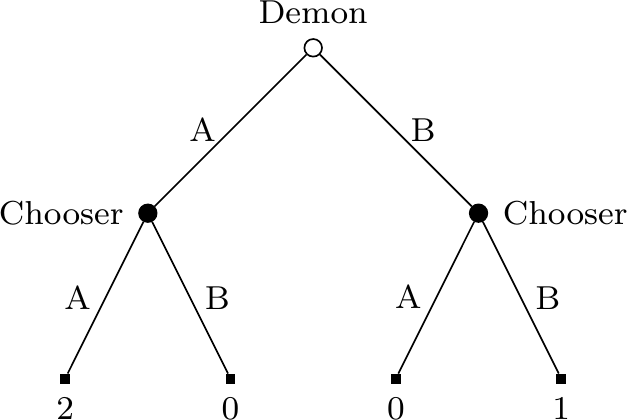
\includegraphics{dual_files/figure-pdf/fig-subgame-example-1.png}

}

\caption{\label{fig-subgame-example}Tree Diagram of the Non-Equivalence
Game.}

\end{figure}

Here is how to understand graphs like Figure~\ref{fig-subgame-example}.
The circles are nodes where one or other player (Chooser, Demon, or
Nature) has to make a choice. The open circle, here at the top of the
tree, is the first such choice. Where possible, I'll draw trees where
later choices are lower on the page than earlier choices, but this isn't
always possible. What is always the case is that the open circle is the
opening move. The small square nodes are terminal nodes; at that point
the game ends, and Chooser collects their payout.

The strategic form of this game is given in
Table~\ref{tbl-subgame-example}. Demon clearly has two strategies, PA
and PB. But Chooser has four; since they have to plan for a binary
choice in two possibilities. I've written LXRY for the strategy of doing
X on the left hand part of the tree, i.e., if Demon predicts A, and
doing Y on the right hand part of the tree, i.e., if Demon predicts B.

\hypertarget{tbl-subgame-example}{}
\begin{longtable}[]{@{}ccc@{}}
\caption{\label{tbl-subgame-example}Strategic form of the
Non-Equivalence Game}\tabularnewline
\toprule\noalign{}
& PA & PB \\
\midrule\noalign{}
\endfirsthead
\toprule\noalign{}
& PA & PB \\
\midrule\noalign{}
\endhead
\bottomrule\noalign{}
\endlastfoot
\textbf{LARA} & 2 & 0 \\
\textbf{LARB} & 2 & 1 \\
\textbf{LBRA} & 0 & 0 \\
\textbf{LBRB} & 0 & 1 \\
\end{longtable}

The argument against Strategic Form - Extensive Form Equivalence is now
fairly simple. In Figure~\ref{fig-subgame-example}, there is only one
rational choice: LARB. Whatever happens, Chooser has an option between
getting something and getting nothing, and it's better to get something
than nothing. But in Table~\ref{tbl-subgame-example}, there are many
rational choices. The pair of Chooser playing LARA and Demon playing PA
is a Nash equilibrium. If one's theory of rational choice for strategic
games is that any Nash equilibrium is rational, then playing LARA in
Table~\ref{tbl-subgame-example} is rational. Hence different strategies
are rational in Figure~\ref{fig-subgame-example} and
Table~\ref{tbl-subgame-example}, so Equivalence fails.

There are a bunch of ways one could reply to this. One could argue that
in fact LARA is rational in Figure~\ref{fig-subgame-example}. We'll see
a theory that says that in Section~\ref{sec-against-pure-strategy}. One
could argue that LARB is the only rational play in
Table~\ref{tbl-subgame-example}. This possibility complicates the
dialectic around here, because while GDT \emph{rejects} Equivalence, it
also rejects this example. It agrees that LARB is the only rational
choice in Table~\ref{tbl-subgame-example}, because it weakly dominates
LARA.\footnote{I'll discuss this more at length in
  Chapter~\ref{sec-weak}.} The examples that motivate rejecting
Equivalence within GDT are more complicated, and I'll come back to them
in Section~\ref{sec-against-equivalence}.

Note that to save Equivalence, it's not enough to merely deny that there
are multiple permissible moves in Table~\ref{tbl-subgame-example}.
Evidential Decision Theory says that there is only one rational move in
that game, and it's LARA. That has an expected return of 2, while LARB
has an expected return of 1.5. But EDT agrees that in
Figure~\ref{fig-subgame-example}, the only rational strategy is LARB. So
EDT agrees with the game theory textbooks that this is a counterexample
to Equivalence, even though it disagrees about why it is a
counterexample.

\hypertarget{sec-four-options}{%
\section{Four Options}\label{sec-four-options}}

\hypertarget{sec-contestants}{%
\subsection{Introducing the Contestants}\label{sec-contestants}}

I've already briefly alluded to these, but it's time to set out in more
detail the four approaches to dynamic choice that I'll consider at
greater length over this chapter.

\textbf{Purely Strategic} approaches say that Chooser uses decision
theory to choose a strategy, and then implements that strategy at each
node. This is sometimes known in philosophy as the resolute approach to
decision theory.\footnote{That particular term, `resolute', is
  associated with a view that Edward McClennen developed to deal with
  cases of foreseeable changes of preference
  (\protect\hyperlink{ref-McClennen1990}{McClennan 1990b}). As already
  indicated, I'm just looking at games where preferences do not change
  over the game.} In a finite game, there will be finitely many
strategies. This finite number may be very large, but it can be
calculated. And similarly there are finitely many strategies for each of
the non-human players, and Chooser can work out the conditional
probability for each such strategy given their choice of strategy. So we
have a very large, but finite, game, and most decision theories on the
market in philosophy will have something to say about what Chooser
should do in this large game. All that's then left to do is to carry the
strategy out.

\textbf{Purely Consequentialist} approaches say that Chooser will
consider every decision at a node on its own merits, solely thinking
about the consequences of that particular decision. This is sometimes
called the `sophisticated' approach to dynamic choice in philosophical
discussions, but I prefer calling it the Purely Consequentialist
approach. I don't like the implicit endorsement in calling something
sophisticated, and given that I've already called the rival approach
strategic, having two names starting with the same letter is bad. The
name I'm using echoes the influential understanding of consequentialism
in Hammond (\protect\hyperlink{ref-Hammond1988}{1988}). And it gets at
what is important about the view; that it rules out looking back.

If Chooser is Purely Consequentialist and they face a series of choices,
they will work backwards.\footnote{See the discussion of backward
  induction on pages 80ff of Bonanno
  (\protect\hyperlink{ref-Bonanno2018}{2018}).} They will work out what
they will do at terminal stages of the game, i.e., at stages where they
will have no more decisions whatever they do. When they are making a
decision at a non-terminal stage, they will treat their own future
decisions as something to be predicted, not planned for. So they will
have a probability distribution over the possible choices, and act as if
Nature is (randomly) selecting which choice. Now we've stipulated that
Chooser knows they will be rational in future stages, so in cases where
there is only one rational choice, Chooser will assign probability 1 to
them making that choice, and 0 to the alternatives. But in the cases
where there are multiple options that are rationally permissible, this
probability assignment might be more interesting, and I'll have more to
say in Section~\ref{sec-against-pure-consequence} about the effects of
this.

\textbf{Equivalence} approaches say that Chooser does not have to adopt
one or other of these approaches, because once we have the right theory
of choice in one-shot games, it will turn out that the two approaches
issue in the same verdicts. That is, it will turn out that Strategic
Form - Normal Form Equivalence is true. Robert Stalnaker
(\protect\hyperlink{ref-Stalnaker1999}{1999}) defends this view in game
theory. I'll argue that the differences between demonic decisions
problems and games are just big enough that his defence can't be adopted
to the puzzles I'm looking at.\footnote{This is just about the only
  place in the book where I'll rely on a \emph{disanalogy} between
  decision theory and game theory.}

Finally, the \textbf{Dual Mandate} approach says that both of the first
two approaches were partly correct. Both of them correctly state
necessary conditions for rational action. Where they go wrong is the
`pure' part, i.e., by saying that these are sufficient conditions for
rational action. And that's what GDT says, and what I'm going to defend.

\hypertarget{sec-four-pictures}{%
\subsection{Picturing the Views}\label{sec-four-pictures}}

Chooser has to act now, and which action is best depends in part on what
they'll do tomorrow? How should they think of tomorrow's action?

Not as something they can control; they are a free and rational agent,
who can't simply be bound.

Not as something like the weather that they can merely predict; they
don't see themselves as simply a thing to be predicted.

Quote Stalnaker at length, can't remember which paper.

Agree - we need something in between.

Strategic views as Strangelove; I bind myself into a position, the
position that I would most like to be bound into.

Consequentialist views as Zaphod; future me is just this guy.

Neither is good.

\hypertarget{sec-binding}{%
\subsection{Binding}\label{sec-binding}}

Is it part of our theory of rationality that people can bind themselves?

Quote Spencer on this.

Not a great argument; even if we can't bind, maybe ideal people can.

But it seems, and this is a judgment call, that we don't get any extra
explanatory power from doing that. Maybe we do, but most people will
give up on plans that they are sure have failed, if the stakes are high
enough.

GDT view: people can bind themselves to plans that make sense. If asked
now whether I want to bet on heads or tails in an hour, I can bind
myself to heads. I can form an intention, in the Bratman-Holton sense,
to bet on heads, and simply carry it out. What was permissible, betting
on tails, becomes impermissible. That seems to be possible, and add
predictive weight.

In normal theories, this is just a weird edge case. Who cares? But for
GDT, it's the main case, since there are lots of times there are
multiple permissible options.

\hypertarget{sec-against-equivalence}{%
\section{Against Equivalence}\label{sec-against-equivalence}}

I'll start with arguing against Equivalence. This is the view that we
don't have to choose between Strategic and Consequentialist approaches
to dynamic choice, because once we get the details of each theory right,
we'll see that they are equivalent.

Earlier I mentioned that this is usually rejected in game theory
textbooks on the basis of examples like Figure~\ref{fig-subgame-example}
and Table~\ref{tbl-subgame-example}. The strategic form of that game has
a Nash equilibrium that seems obviously bad to play in the extensive
form of the game.

This is a bad argument against equivalence because it's easy to fix the
theory of strategic choice to avoid the problem. If we say that weakly
dominated strategies are not choice-worthy, then the strategies that can
be rationally chosen in Table~\ref{tbl-subgame-example} are exactly the
strategies that can be rationally played in
Figure~\ref{fig-subgame-example}.

But this only shows that this example is not a counterexample to
Equivalence. It could be that there are other cases that are
counterexamples. Figure~\ref{fig-stalnaker-centipede} is the game tree
(in the sense described in Section~\ref{sec-decision-tree}) for one such
example.

\begin{figure}

{\centering 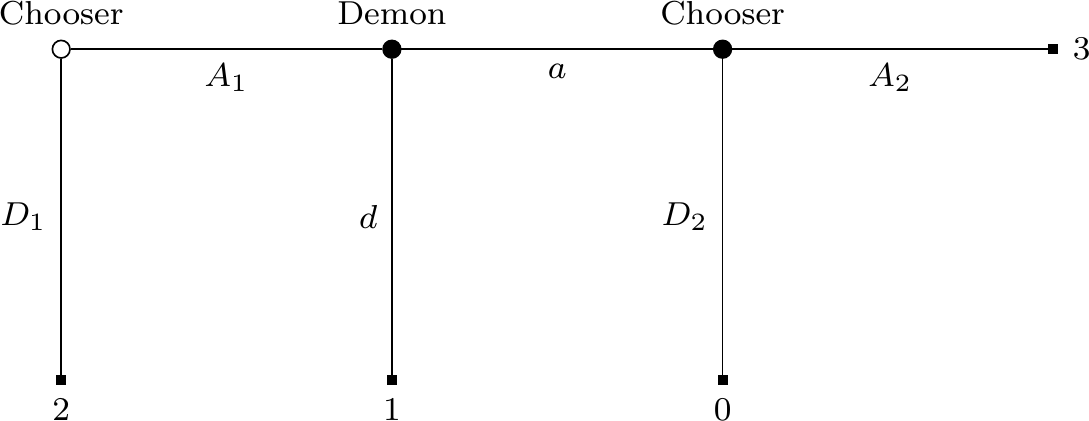
\includegraphics{dual_files/figure-pdf/fig-stalnaker-centipede-1.png}

}

\caption{\label{fig-stalnaker-centipede}Tree Diagram of the Centipede
Game}

\end{figure}

In Figure~\ref{fig-stalnaker-centipede} are three stages, though the
game might end at any stage. Chooser is the mover at stage 1 and, if the
game gets that far, stage 3. Demon is the mover at stage 2, again if the
game gets that far. At stage 1 and 2, if the mover moves down, the game
ends. After stage 3, the game ends either way. Chooser's payouts are
given on the tree. Demon's disposition is to do whatever they predict
Chooser will do at stage 3, and they are arbitrarily good at predicting
Chooser's strategy.\footnote{This problem is very closely modelled on a
  game described by Stalnaker
  (\protect\hyperlink{ref-Stalnaker1998}{1998, 47}). But note that how
  I've described Demon is different to how Stalnaker describes `Bob',
  the player who moves at stage 2 in his version of the game. In his
  version of the game, the player who moves first just knows that the
  player who moves second is rational, and the function they are trying
  to maximise. In my version of the game, the player who moves first
  also knows how the player who moves second will react if they are
  indifferent between their options. That's why I get what appears to be
  a different analysis to Stalnaker; we're not disagreeing here I think,
  just analysing different games.}

In this dynamic game, the only sensible thing for Chooser to do at stage
1 is to play A\textsubscript{1}. That's because they know that if they
get to stage 3, they will play A\textsubscript{2}, getting 3, rather
than D\textsubscript{2}, getting 0.\footnote{I'm assuming here that
  Chooser knows that they will be rational in the future, and this
  knowledge persists no matter what earlier choices they make. This is a
  substantial idealisation, but makes sense given the other
  idealisations that were described in Chapter~\ref{sec-ideal}.} So they
should believe that Demon will predict that they will play
A\textsubscript{2}, and hence will play a. So they should believe at
stage 1 that playing A\textsubscript{1} will get 3, while playing
D\textsubscript{1} will get 2, so they should play A\textsubscript{1} at
stage 1.

None of that should be too surprising; it's the standard backward
induction solution of the game.\footnote{Though I've been a bit more
  careful here about just what assumptions each player can make about
  the other at each stage than is usual.} But now consider what happens
in the strategic form of the game. Chooser has four strategies:
A\textsubscript{1} or D\textsubscript{1}, crossed with
A\textsubscript{2} or D\textsubscript{2}. Let's simply give these
strategies names, as follows.

\hypertarget{tbl-stalnaker-centipede-strategies}{}
\begin{longtable}[]{@{}ccc@{}}
\caption{\label{tbl-stalnaker-centipede-strategies}The possible
strategies for Chooser in
Figure~\ref{fig-stalnaker-centipede}.}\tabularnewline
\toprule\noalign{}
Strategy & Move 1 & Move 2 \\
\midrule\noalign{}
\endfirsthead
\toprule\noalign{}
Strategy & Move 1 & Move 2 \\
\midrule\noalign{}
\endhead
\bottomrule\noalign{}
\endlastfoot
S\textsubscript{1} & D\textsubscript{1} & D\textsubscript{2} \\
S\textsubscript{2} & D\textsubscript{1} & A\textsubscript{2} \\
S\textsubscript{3} & A\textsubscript{1} & D\textsubscript{2} \\
S\textsubscript{4} & A\textsubscript{1} & A\textsubscript{2} \\
\end{longtable}

Then Demon has two moves as well, which I'll call PO and PE. PO means
that Demon predicts that Chooser will play an odd numbered strategy,
i.e., S\textsubscript{1} or S\textsubscript{3}. That is, Demon predicts
that Chooser will play (or be disposed to play) D\textsubscript{2}. So
PO is equivalent to Demon playing (or being disposed to play) d.~PE
means that Demon predicts that Chooser will play an even numbered
strategy, i.e., S\textsubscript{2} or S\textsubscript{4}. That is, Demon
predicts that Chooser will play (or be disposed to play)
A\textsubscript{2}. So PO is equivalent to Demon playing (or being
disposed to play) a. Given that, we can describe the strategic form of
the decision problem. That is, we can set out the strategies for Chooser
and Demon, and say what payout Chooser gets for each possible pair of
choices.

\hypertarget{tbl-stalnaker-centipede}{}
\begin{longtable}[]{@{}ccc@{}}
\caption{\label{tbl-stalnaker-centipede}The strategic form of
Figure~\ref{fig-stalnaker-centipede}.}\tabularnewline
\toprule\noalign{}
& PO & PE \\
\midrule\noalign{}
\endfirsthead
\toprule\noalign{}
& PO & PE \\
\midrule\noalign{}
\endhead
\bottomrule\noalign{}
\endlastfoot
\textbf{S\textsubscript{1}} & 2 & 2 \\
\textbf{S\textsubscript{2}} & 2 & 2 \\
\textbf{S\textsubscript{3}} & 0 & 1 \\
\textbf{S\textsubscript{4}} & 3 & 1 \\
\end{longtable}

If Chooser was making a one-off choice in
Table~\ref{tbl-stalnaker-centipede}, it would be rational, according to
GDT, to choose S\textsubscript{2}. That is ratifiable and not weakly
dominated. It wouldn't be rational to choose S\textsubscript{1}, because
given S\textsubscript{1} it would be better to choose
S\textsubscript{4}. But given S\textsubscript{2} is chosen, it is
optimal, since once S\textsubscript{2} is chosen, Chooser should believe
that Demon is playing PE. So in this one-shot game, where one just
chooses a strategy, it is rational (according to GDT) to play
S\textsubscript{2}.

That's my argument against Equivalence. In
Table~\ref{tbl-stalnaker-centipede} it is rational to choose
S\textsubscript{2}. But in Figure~\ref{fig-stalnaker-centipede} it is
not rational to play that strategy, i.e., to play D\textsubscript{1},
because the backward induction argument for playing A\textsubscript{1}
is sound. So the strategic and extensive forms of the game are not
equivalent.

I could try to turn this into an argument against Purely Strategic
approaches to decision theory as well, using the following reasoning.

\begin{enumerate}
\def\labelenumi{\arabic{enumi}.}
\tightlist
\item
  In Table~\ref{tbl-stalnaker-centipede}, it is rational to play
  S\textsubscript{2}.
\item
  In Figure~\ref{fig-stalnaker-centipede}, it is not rational to play
  S\textsubscript{2}.
\item
  If Purely Strategic approaches to decision theory are correct, then
  the same choices are rational in Table~\ref{tbl-stalnaker-centipede}
  and Figure~\ref{fig-stalnaker-centipede}.
\item
  Therefore, Purely Strategic approaches are incorrect.
\end{enumerate}

But this argument would be blatantly question-begging. The argument for
premise 2 relies on backward induction reasoning, and people who endorse
Purely Strategic reasoning do so because they reject backward induction
reasoning. So it wouldn't be at all convincing. (Probably many people
who endorse Purely Strategic approaches would reject premise 1 as well.)
So in Section~\ref{sec-against-pure-strategy} I'll offer some arguments
against Purely Strategic approaches that are not so obviously
question-begging.

\hypertarget{sec-against-pure-strategy}{%
\section{Against Purely Strategic
Approaches}\label{sec-against-pure-strategy}}

From now on I'll assume that rival theories are rejecting Equivalence,
and rejecting Dual Mandate. So in this section I'll focus on theories
that say the right thing to do is to select a rational strategy, and
then carry it out. And I take it to be part of this theory that
sometimes this means making choices that do not make sense, by the
theory's own lights, if they were `one-off' choices. If there are no
such cases, the theory is either a version of Equivalence, or of the
Dual Mandate.

For this reason, I won't spend any time on versions of Causal Decision
Theory that are Purely Strategic. Such theories would be unmotivated.
Causal Decision Theorists think that in Newcomb's Problem, one reason
that it doesn't make sense to choose the dominated option is that if one
knew what Demon had predicted, one would definitely take the dominating
option. That's to say, they think the fact that one knows that some
choice would be rational given further information is a reason to make
the choice. And that's in tension with the idea that it's rational to
play a strategy that will not make sense when it's being carried out,
just because at the start of the tree it looks like the best strategy.

In practice, defenders of Purely Strategic views do not normally assume
CDT. There are, instead, two main motivations for Purely Strategic
views. One of them won't matter to this project. It is the idea that in
non-ideal settings, particularly when preferences might change, or one
might be irrational later, it might be better to simply choose a
strategy and stick to it. Since I'm only talking about ideal theory
here, I'll set that aside. The other motivation is more interesting. It
is that the reasons behind Evidential Decision Theory (EDT) are in fact
better reasons to choose Strategic Evidential Decision Theory (SEDT).

SEDT is a fairly simple theory. It has two rules.

\begin{enumerate}
\def\labelenumi{\arabic{enumi}.}
\tightlist
\item
  In dynamic choices, one should choose an optimal strategy at the start
  of the tree, and carry that strategy out the rest of the way.
\item
  The right way to evaluate strategies is to use Evidential Decision
  Theory.
\end{enumerate}

SEDT is very similar to the Functional Decision Theory defended by
Levinstein and Soares
(\protect\hyperlink{ref-LevinsteinSoares2020}{2020}). My excuses for
using a new name are that (a) this name is a little more descriptive,
and (b) I'm not quite sure that the theories are the same. I think they
say the same things about every case I'll discuss in this section, but
Levinstein and Soares don't discuss cases of demons who make imperfect
predictions, so I'm guessing a little bit about what they'd say. And
possibly my understanding of what a single decision problem is doesn't
exactly match theirs. So rather than do more exegesis, I'll focus on
SEDT, which is in any case an interesting theory.

One way to motivate SEDT is by thinking about a version of
\protect\hyperlink{tbl-newcomb}{Newcomb's Problem} where Demon's
predictions are revealed to Chooser. The game tree for this variant on
Newcomb's Problem is in Figure~\ref{fig-open-newcomb}.

\begin{figure}

{\centering 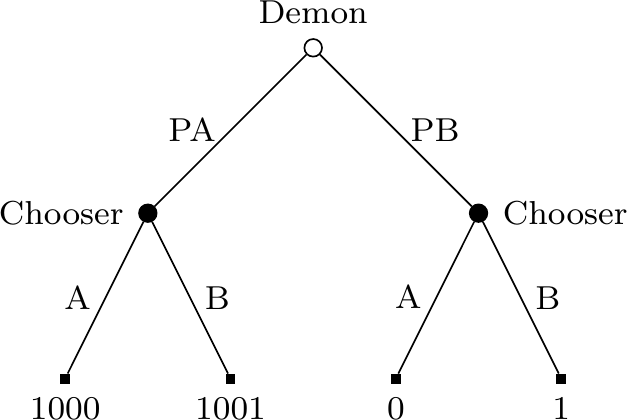
\includegraphics{dual_files/figure-pdf/fig-open-newcomb-1.png}

}

\caption{\label{fig-open-newcomb}Tree Diagram of the Open Newcomb game.}

\end{figure}

In Figure~\ref{fig-open-newcomb}, regular EDT says to choose B. After
all, no matter which node one is at, the best thing to do given that one
is there is to take the extra 1 on offer. But it's surprisingly hard to
come up with reasons to choose A in the original problem that do not
extend to this problem. The main reason which is offered, that people
who choose A end up richer, applies equally well here. And the main
objection that opponents make, that choosing A is strange because one
knows that one would choose B once one discovered what prediction was
made, does not have any bite if one would follow SEDT and not in fact
choose B were the prediction revealed.

It's a little amusing to imagine a proponent of regular EDT playing a
version of Figure~\ref{fig-open-newcomb}. Presumably they would do
whatever they could to not learn what the prediction was until they
could make a choice. After all, by their own lights, learning what the
prediction was would cost them, in expectation, 999. So depending on how
this information will be revealed, they will close their eyes, sing ``La
la la I can't hear you'' to block out noises, maybe hold their breath if
the information will be revealed by distinctive smells, and so on. This
doesn't seem like an image of a practically rational Chooser, and SEDT
avoids all these problems.

That's not to say that SEDT is entirely without its own intuitive costs,
even in simple cases like Figure~\ref{fig-open-newcomb}. The person
carrying out SEDT will give the following speech. ``I am not here to be
a hero; I'm not following some philosophical theory just because it's
cool. My job is making money. And, now that the prediction is revealed,
I can see that I'll make more money choosing B. But I'm taking A.''
Again, this doesn't sound great. But, they argue, it does in fact lead
to getting more money, on average, so maybe there is something to it.
And SEDT does not agree with EDT in the cases I described in
Section~\ref{sec-war-on-war}, so I can't say that they are relying, as
EDT relies, on too narrow a diet of cases.

Still, SEDT is not defensible in all somewhat realistic situations. The
example I'll use to demonstrate this is rather more violent than the
other examples in this book. But it needs to be rather violent in order
to rule out the possibility of there being strategic or reputational
considerations that are being left out.

Chooser is the Prime Minister of a small country, and they are
threatened by a large nearby country, Neighbour. Unfortunately,
Neighbour is thinking of carpet bombing Chooser's capital, in
retaliation for some perceived slight during trade negotiations. Chooser
has no air defences to stop the bombing, and no allies who will rally to
help.

Fortunately, Chooser has a mighty weapon, a Doomsday device, that could
destroy Neighbour. Chooser has obviously threatened to use this, but
Neighbour suspects it is a bluff. This is for a good reason; the
doomsday device would also destroy Chooser's own country. Neighbour is
known to employ Demon who is at least 99\% accurate in predicting what
military plans Chooser will take.\footnote{It's very important to this
  example that Demon is not perfectly accurate. There hasn't been as
  much attention as there might have been to what happens to theories
  like SEDT in the context of good but not perfect Demons.

  One might worry that the case is not, as promised, realistic, because
  states do not in fact have Demons. That's true, but they do have
  spies, and analysts, and they are somewhat reliable in making
  predictions. It seems plausible that they could be reliable enough to
  get the case to work.} In practice, all Demon has to do is predict So
Chooser can do Nothing (N), or use the Doomsday device (D), should
neighbour attack. Chooser would obviously prefer no attack, and would
certainly not use the device preemptively. And Neighbour will attack iff
Demon predicts that Chooser will do Nothing. Given all that the decision
table that Chooser faces is in Table~\ref{tbl-retaliation}.

\hypertarget{tbl-retaliation}{}
\begin{longtable}[]{@{}ccc@{}}
\caption{\label{tbl-retaliation}Deciding whether to
retaliate.}\tabularnewline
\toprule\noalign{}
& PN & PD \\
\midrule\noalign{}
\endfirsthead
\toprule\noalign{}
& PN & PD \\
\midrule\noalign{}
\endhead
\bottomrule\noalign{}
\endlastfoot
\textbf{N} & -1 & 0 \\
\textbf{D} & -50 & 0 \\
\end{longtable}

In the top left, Neighbour bombs Chooser's capital, thinking correctly
that Chooser will not retaliate. In the top right and lower right,
neighbour is sufficiently scared of the doomsday device that they do
nothing. But in the bottom left, Neighbour attacks, and Chooser
retaliates, creating a disaster for everyone, something 50 times worse
than even the horrors of the carpet bombing.

Still, if Chooser is picking a strategy before anything starts, the
strategy with the highest value, according to EDT, is to plan to use the
Doomsday device. This has an expected return of -0.5; since one time in
a hundred it returns -50, and otherwise it returns 0. That's what SEDT
says one should do. And it says Chooser should quite literally stick to
their guns, even if they see the bombers coming, and they realise their
bluff has failed.

This seems absurd to me, and it is the kind of result that drives game
theorists to the dual mandate. In case that example isn't decisive
enough, let's consider two more variants on it.

Change the example so that Chooser has two advisors who are talking to
them as the bombers come in. One of them says that the Demon is 99\%
reliable. The other says that the Demon is 97\% reliable. Whether
Chooser launches the Doomsday device should, according to SEDT, depend
on which advisor Chooser believes. This is just absurd. A debate about
the general accuracy of a Demon can't possibly be what these grave
military decisions are based on.

Change the example again, and make it a bit more realistic. Chooser has
the same two advisors, with the same views. Chooser thinks the one who
says the Demon is 99\% reliable is 60\% likely to be right, and the
other 40\% likely. So Chooser forms the plan use the Doomsday device,
because right now that's the strategy with highest expected return. But
having made that decision, much to everyone's surprise, Neighbour
attacks. SEDT now says to launch the Doomsday device.

But think about how the choice of plans looks to Chooser now. The
actions of Neighbour are evidence about the reliability of Demon. And a
simple application of Bayes' Rule says that Chooser should now think the
advisor who thought the demon was 97\% reliable is 2/3 likely to be
right. That is, given Chooser's current evidence merely about the
Demon's reliability (and not about what the Demon actually did), SEDT
says not to use the Doomsday device. Yet despite it not being either the
utility maximising strategy, or the utility maximising choice, SEDT says
to launch the Doomsday device. This seems completely absurd, and enough
to have us move to a new theory.

\hypertarget{sec-against-pure-consequence}{%
\section{Against Purely Consequentialist
Approaches}\label{sec-against-pure-consequence}}

\begin{figure}

{\centering 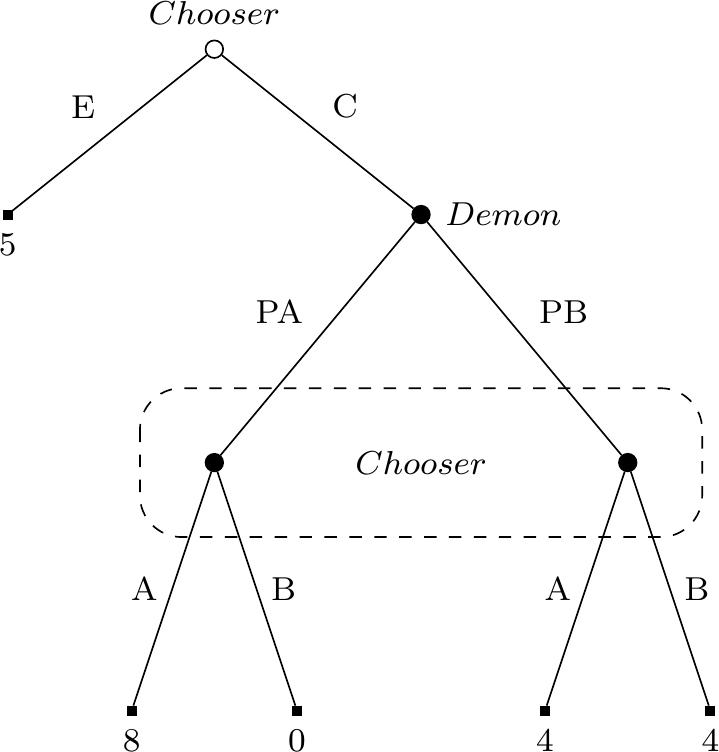
\includegraphics{dual_files/figure-pdf/fig-against-consequence-1.png}

}

\caption{\label{fig-against-consequence}Tree Diagram of the Open Newcomb
game.}

\end{figure}

\hypertarget{tbl-against-consequence-short}{}
\begin{longtable}[]{@{}ccc@{}}
\caption{\label{tbl-against-consequence-short}The second round game in
Figure~\ref{fig-against-consequence}.}\tabularnewline
\toprule\noalign{}
& PA & PB \\
\midrule\noalign{}
\endfirsthead
\toprule\noalign{}
& PA & PB \\
\midrule\noalign{}
\endhead
\bottomrule\noalign{}
\endlastfoot
\textbf{A} & 8 & 0 \\
\textbf{B} & 4 & 4 \\
\end{longtable}

\hypertarget{tbl-against-consequence-long}{}
\begin{longtable}[]{@{}ccc@{}}
\caption{\label{tbl-against-consequence-long}The strategy table for
Figure~\ref{fig-against-consequence}.}\tabularnewline
\toprule\noalign{}
& PA & PB \\
\midrule\noalign{}
\endfirsthead
\toprule\noalign{}
& PA & PB \\
\midrule\noalign{}
\endhead
\bottomrule\noalign{}
\endlastfoot
\textbf{EA} & 5 & 5 \\
\textbf{EB} & 5 & 5 \\
\textbf{CA} & 8 & 0 \\
\textbf{CB} & 4 & 4 \\
\end{longtable}

First against CEDT - breaches the spirit of EDT.

Then against Gallow + Consequence: Could lead to choosing dominated
option.

What about Hunting + Consequence? Not sure I have an argument there.

This has an important technical consequence: Purely Consequentialist
theories are \emph{unstable} in the sense Dmitri Gallow
(\protect\hyperlink{ref-Gallownd}{n.d.}) has described. If the pure
consequentialist changes their own probability distribution over what
they will do, what act is rational for them changes.\footnote{The point
  here is somewhat connected to the point Bonanno makes about how
  backwards induction works in games where a player is indifferent
  between certain outcomes (\protect\hyperlink{ref-Bonanno2018}{Bonanno
  2018, 80ff}).} I don't think this is ever an issue for CEDT, but it is
an issue for other Purely Consequentialist theories. For instance, GDT
says that either A or B is a permissible choice in
Table~\ref{tbl-first-dynamic-example}.

\bookmarksetup{startatroot}

\hypertarget{sec-indecisive}{%
\chapter{Indecisive}\label{sec-indecisive}}

Game theory is full of \emph{solution concepts}; ideas for how to solve
a game. That is, they are methods for determining the possible outcomes
of a game played by rational players. Compared to philosophical decision
theory, there are two big things to know about these solution concepts.
One is that there are many of them. It isn't like having a single theory
to rule all cases. More complex theories tend to give more intuitive
results on more cases. But the complexity is a cost, and in any case no
theory gets all the intuitions about all the cases. The other thing is
that these will often say that there are multiple possible outcomes for
a game, and that knowing the players are rational doesn't suffice to
know what they will do. It's this latter feature of game theory that
I'll argue here decision theory should imitate.

Say that a theory is \emph{indecisive} if for at least one problem it
says there are at least two options such that both are rationally
permissible, and the options are not equally good. And say, following
Ruth Chang (\protect\hyperlink{ref-Chang2002}{2002}), that two options
are equally good if improving either of them by a small amount epsilon
would make that one better, i.e., would make it the only permissible
choice. So an indecisive theory says that sometimes, multiple choices
are permissible, and stay permissible after one or other is sweetened by
a small improvement. The vast majority of decision theories on the
market are decisive. That's because they first assign a numerical value
to each option, and say to choose with the highest value. This allows
multiple options iff multiple choices have the same numerical value. But
sweetenings increase the value, so they destroy equality and hence the
permissibility of each choice.

Perhaps the most intuitive case for indecisiveness involves what I'll
call Stag Hunt decisions.\footnote{For much more on the philosophical
  importance of Stag Hunts, see Skyrms
  (\protect\hyperlink{ref-Skyrms2004}{2004}).} Here is an example of a
Stag Hunt decision.

\hypertarget{tbl-stag-hunt}{}
\begin{longtable}[]{@{}ccc@{}}
\caption{\label{tbl-stag-hunt}An example of a Stag Hunt.}\tabularnewline
\toprule\noalign{}
\endfirsthead
\endhead
\bottomrule\noalign{}
\endlastfoot
& \textbf{PUp} & \textbf{PDown} \\
\textbf{Up} & 6 & 0 \\
\textbf{Down} & 5 & 2 \\
\end{longtable}

Note three things about this game. First, both Up and Down are
ratifiable. Second, Up has a higher expected return than Down. Third, Up
has a higher possible regret than Down. If Chooser plays Up and Demon is
wrong, Chooser gets 2 less than they might have otherwise. (They get 0
but could have got 2.) If Chooser plays Down and Demon is wrong, Chooser
only gets 1 less than they might have otherwise. (They get 5 but could
have got 6.)

There is considerable disagreement about what this means for Chooser.
EDT says that Chooser should play Up, as does the ratifiable variant of
EDT in Jeffrey (\protect\hyperlink{ref-Jeffrey1983}{1983}), and some
causal decision theorists such as Arntzenius
(\protect\hyperlink{ref-Arntzenius2008}{2008}) and Gustafsson
(\protect\hyperlink{ref-Gustafsson2011}{2011}). On the other hand,
several other theorists who endorse two-boxing in Newcomb's Problem,
like Wedgwood (\protect\hyperlink{ref-Wedgwood2013a}{2013}), Gallow
(\protect\hyperlink{ref-Gallow2020}{2020}), Podgorski
(\protect\hyperlink{ref-Podgorski2022}{2022}), and Barnett
(\protect\hyperlink{ref-Barnett2022}{2022}), endorse playing Down on the
ground of regret miminisation. I think both Up and Down are
permissible.\footnote{The view I'm going to develop is hence similar to
  the `permissive CDT' defended by Fusco
  (\protect\hyperlink{ref-Fuscond}{n.d.}).} I also think this is the
intuitively right verdict, though I place no weight on that intuition.
In general, I think in any problem that has the three features described
in the last paragraph (two equilibria, one better according to EDT, the
other with lower possible regret), either option is permissible. Since
lightly sweetening either Up or Down in this problem doesn't change
either feature, that is why my theory is indecisive.

My argument for indecisiveness will turn on a case that all seven of the
views mentioned in the last paragraph agree on, namely
Table~\ref{tbl-coord}.

\hypertarget{tbl-coord}{}
\begin{longtable}[]{@{}ccc@{}}
\caption{\label{tbl-coord}An example of a coordination
game.}\tabularnewline
\toprule\noalign{}
\endfirsthead
\endhead
\bottomrule\noalign{}
\endlastfoot
& \textbf{PUp} & \textbf{PDown} \\
\textbf{Up} & 4 & 0 \\
\textbf{Down} & 0 & 3 \\
\end{longtable}

All of them agree that Up is the uniquely rational play in this example,
and I think intuition agrees with them. I'll argue, however, that Down
is permissible. The argument turns on a variation that embeds cite table
in a more complicated problem. This problem involves two demons, each of
whom are arbitrarily good at predicting Chooser. The (first version of)
the problem involves the following sequence.

\begin{enumerate}
\def\labelenumi{\arabic{enumi}.}
\tightlist
\item
  Both Demon-1 and Demon-2 predict Chooser, but do not reveal their
  prediction.
\item
  If Demon-1 predicts Chooser plays Up, they Exit with probability 0.5,
  and Chooser gets 0. If Demon-1 predicts Chooser plays Down, they do
  not Exit. (That is, they Exit with probability 0.) If they Exit, the
  problem ends, and Chooser is told this. Otherwise, we go to the next
  step.
\item
  Chooser chooses Up or Down.
\item
  Demon-2's prediction is chosen, and that determines whether we are in
  state PU or state PD.
\item
  Chooser's payouts are given by cite above table.
\end{enumerate}

I'll call these Exit Problems, and Table~\ref{tbl-general-exit} gives
the general form of such a problem. Our problem has this abstract of
Table~\ref{tbl-general-exit} with \emph{b} = \emph{c} = \emph{e} =
\emph{y} = 0, \emph{x} = 0.5, \emph{a} = 4, \emph{d} = 3.

\begin{table}

\caption{\label{tbl-general-exit}The abstract form of an exit
problem.}\begin{minipage}[t]{0.50\linewidth}
\subcaption{\label{tbl-exit-param}Exit Parameters}

{\centering 

\begin{tabular}[t]{cc}
\toprule
Exit Payout & \emph{e}\\
Pr(Exit \textbar{} PUp) & \emph{x}\\
Pr(Exit \textbar{} PDown) & \emph{y}\\
\bottomrule
\end{tabular}

}

\end{minipage}%
%
\begin{minipage}[t]{0.50\linewidth}
\subcaption{\label{tbl-exit-r2g}Round 2 game}

{\centering 

\begin{tabular}[t]{ccc}
\toprule
 & \textbf{PUp} & \textbf{PDown}\\
\textbf{Up} & \emph{a} & \emph{b}\\
\textbf{Down} & \emph{c} & \emph{d}\\
\bottomrule
\end{tabular}

}

\end{minipage}%

\end{table}

Now consider a simple variant of the above 5 step problem. The same
things happen, but steps 2 and 3 are reversed. That is, Chooser decides
on Up or Down after Demons make their predictions, but before they are
told whether Demon-1 decided to Exit. Still, their choice will only
matter if Demon-1 decided not to Exit, since their choices do not make a
difference if Demon-1 Exits. Call this variant the Early Choice version,
and the original the Late Choice variant. I don't have any clear
intuitions about what to do in most Exit Problems, save for this
constraint on choices.

\begin{itemize}
\tightlist
\item
  \textbf{Exit Principle}: In any Exit Problem, the same choices are
  permissible in the Early Choice and Late Choice variants.
\end{itemize}

The reason comes from thinking about what Chooser is doing in the Early
Choice variant. They are making a decision about what to do if Demon-1
doesn't Exit. The way to make that decision is just to assume that
Demon-1 doesn't Exit, and then decide what to do. It just is the same
choice as they face in the Late Choice variant, except now they make it
in the context of a conditional. So they should decide it the same way.

To put the point in game-theoretic terms, there is no difference between
extensive form and normal form reasoning when a decider has only one
possible choice to make. And there is a natural argument for this claim.
It starts with the idea that for any \emph{p}, the following two
questions have the same answers.

\begin{enumerate}
\def\labelenumi{\arabic{enumi}.}
\tightlist
\item
  If \emph{p} happens, what do you want to do?
\item
  So, \emph{p} happened. What do you want to do?
\end{enumerate}

When one is asked to choose a strategy for a tree that has only one
possible decision in it, the question one is being asked is that if we
get to the point in the tree where one has to decide, what will you do.
And the `Late Question' is that that point in the tree has been reached;
now what will you do? So the questions fit the schema, and should get
the same answers. One could see this as a consequence of applying
something like the Ramsey test to conditional questions
(\protect\hyperlink{ref-RamseyGeneralProp}{Ramsey 1990}). Denying Exit
Principle means treating these two very similar sounding questions
differently, and that's implausible.

One could also argue, I think correctly, that anyone who violates Exit
Principle will violate a plausible version of the Sure Thing
Principle.\footnote{To be sure, it's not entirely clear how to even
  state the Sure Thing Principle in the framework of causal
  ratificationism. Ratificationism does not output a preference ordering
  over options; it just says which options are and are not
  choice-worthy. And exactly how to translate principles like Sure Thing
  that are usually stated in terms of preference to ones in terms of
  choiceworthiness isn't always clear. One consequence of this is that I
  don't want to lean on Sure Thing as a premise. Another is that
  ratificationism isn't really subject to the objections that Gallow
  (\protect\hyperlink{ref-Gallownd}{n.d.}) makes to theories that
  endorse Sure Thing, since the version of Sure Thing he uses is stated
  in terms of preferences. (Officially, ratificationism is `unstable' in
  his sense because it doesn't output a preference ordering over
  unchosen options; that doesn't seem like a weakness to me.)} Such an
argument seems sound to me, but the Sure Thing Principle is
controversial, and I prefer to put more weight on the argument from how
conditional reasoning works in the previous paragraph. (Indeed, I think
using the Exit Principle to motivate a version of the Sure Thing
Principle is more plausible than the reverse argument.)

Any plausible theory that says that only Up is rationally playable in
problems like Table~\ref{tbl-coord} cite above table will violate Exit
Principle. Think about what they will say Table~\ref{tbl-early-choice}.

\hypertarget{tbl-early-choice}{}
\begin{longtable}[]{@{}cccc@{}}
\caption{\label{tbl-early-choice}The Early Choice
decision.}\tabularnewline
\toprule\noalign{}
\endfirsthead
\endhead
\bottomrule\noalign{}
\endlastfoot
& \textbf{PUp} & \textbf{PMixed} & \textbf{PDown} \\
\textbf{Up} & 2 & 3 & 0 \\
\textbf{Down} & 0 & 3 & 3 \\
\end{longtable}

In this problem, PUp means that both demons predict Up, PDown means that
they both predict Down, and PMixed means that one predicts one, and one
the other. This possibility is arbitrarily improbable, and the two
strategies have the same expected return given M in any case, so we can
ignore it. So really this game comes to
Table~\ref{tbl-early-choice-simplified}.

\hypertarget{tbl-early-choice-simplified}{}
\begin{longtable}[]{@{}ccc@{}}
\caption{\label{tbl-early-choice-simplified}The Early Choice decision
simplified.}\tabularnewline
\toprule\noalign{}
\endfirsthead
\endhead
\bottomrule\noalign{}
\endlastfoot
& \textbf{PUp} & \textbf{PDown} \\
\textbf{Up} & 2 & 0 \\
\textbf{Down} & 0 & 3 \\
\end{longtable}

Now presumably if one prefers Up in above table, it is because one
prefers Up in any game like Table~\ref{tbl-general-coord} Table below
where \emph{x} \textgreater{} \emph{y} \textgreater{} 0.

\hypertarget{tbl-general-coord}{}
\begin{longtable}[]{@{}ccc@{}}
\caption{\label{tbl-general-coord}General coordination
game.}\tabularnewline
\toprule\noalign{}
\endfirsthead
\endhead
\bottomrule\noalign{}
\endlastfoot
& \textbf{PUp} & \textbf{PDown} \\
\textbf{Up} & \emph{x} & 0 \\
\textbf{Down} & 0 & \emph{y} \\
\end{longtable}

How could it be otherwise? Given expectationism, it's not like there is
anything special about the numbers 4 and 3. But anyone who endorses this
policy will play Down Table~\ref{tbl-early-choice-simplified} and so,
presumably, in Table~\ref{tbl-early-choice}. And that means they will
violate Exit Principle.

The only view that is consistent with Exit Principle in cases like
Table~\ref{tbl-general-coord} is that both Up and Down are permissible.
And since in any such case, improving Up or Down be a tiny amount
wouldn't materially change the case, they must both be permissible after
small sweetenings. So, given Exit Principle, the only viable theories
are indecisive.

Exit Principle also offers a response to some intuitions that have led
people to question CDT in recent years.
Table~\ref{tbl-frustrating-button} is an example that Jack Spencer
(\protect\hyperlink{ref-Spencer2023}{2023}) used to model the kind of
case that's at issue. As he notes, it is similar to the psychopath
button case (\protect\hyperlink{ref-Egan2007-EGASCT}{Egan 2007b}), the
asymmetric Death in Damascus case
(\protect\hyperlink{ref-Richter1984}{Richter 1984}), and other puzzles
for CDT.

\hypertarget{tbl-frustrating-button}{}
\begin{longtable}[]{@{}ccc@{}}
\caption{\label{tbl-frustrating-button}Frustrating Button (from Spencer
(\protect\hyperlink{ref-Spencer2023}{2023})).}\tabularnewline
\toprule\noalign{}
\endfirsthead
\endhead
\bottomrule\noalign{}
\endlastfoot
& \textbf{PUp} & \textbf{PDown} \\
\textbf{Up} & 10 & 10 \\
\textbf{Down} & 15 & 0 \\
\end{longtable}

Apparently the common intuition here is that that Up is the uniquely
rational play. Note though that if we embed Frustrating Button in an
exit problem, as in Table~\ref{tbl-frustrating-exit}, the intuitions
shift.

\begin{table}

\caption{\label{tbl-frustrating-exit}An exit problem with Frustrating
Button in round 2.}\begin{minipage}[t]{0.50\linewidth}
\subcaption{\label{tbl-exit-param-fb}Exit Parameters}

{\centering 

\begin{tabular}[t]{cc}
\toprule
Exit Payout & -50\\
Pr(Exit \textbar{} PUp) & 0.8\\
Pr(Exit \textbar{} PDown) & 0\\
\bottomrule
\end{tabular}

}

\end{minipage}%
%
\begin{minipage}[t]{0.50\linewidth}
\subcaption{\label{tbl-exit-r2g-fb}Frustrating Button}

{\centering 

\begin{tabular}[t]{ccc}
\toprule
 & \textbf{PUp} & \textbf{PDown}\\
\textbf{Up} & 10 & 10\\
\textbf{Down} & 15 & 0\\
\bottomrule
\end{tabular}

}

\end{minipage}%

\end{table}

The Early Version of Table~\ref{tbl-frustrating-exit} is
Table~\ref{tbl-ev-fe}.

\hypertarget{tbl-ev-fe}{}
\begin{longtable}[]{@{}ccc@{}}
\caption{\label{tbl-ev-fe}Early Version of
Table~\ref{tbl-frustrating-exit}.}\tabularnewline
\toprule\noalign{}
\endfirsthead
\endhead
\bottomrule\noalign{}
\endlastfoot
& \textbf{PUp} & \textbf{PDown} \\
\textbf{Up} & -38 & 10 \\
\textbf{Down} & -37 & 0 \\
\end{longtable}

\newpage

And if there is an intuition here, it is that it's better to choose Down
rather than Up.\footnote{The theory offered in Spencer
  (\protect\hyperlink{ref-Spencer2021b}{2021}) agrees with intuition
  here.} This violates Exit Principle, and it seems incoherent to say
that one would choose Down in this game, when Down just means playing
Down in round 2, and if one were to reach round 2, one would prefer Up.

Exit Principle can also be used to argue against the non-expectationist
theory offered by Lara Buchak
(\protect\hyperlink{ref-BuchakRisk}{2013}), but that argument is more
complicated, and I'll leave it to Appendix Two.

\bookmarksetup{startatroot}

\hypertarget{sec-select}{%
\chapter{Selection}\label{sec-select}}

Some decision theories, most notably EDT, output a valuation of all
possible choices. From that valuation a preference function over choices
can be easily generated; choices that are more highly valued are
preferred to those that are less highly valued. Indeed, that preference
ordering will be a total preorder. Other theories, especially the
theories that recommend Gathering in Stag Decisions, do not output
valuations of all choices, but they do output a preference ordering over
all choices. In some cases that is a total preorder, but often it is
simply a preorder. Still, they share with EDT the idea that a decision
theory outputs a preference ordering over the choices.

GDT rejects this assumption. The aim of a decision theory is to say what
the idealised chooser will choose, given some options. It is not to say
that this unchosen option is 7th best, and that unchosen one is 9th
best. It can't be that, because these claims don't explain behaviour,
and explaining behaviour is the aim of the project. One does not behave
differently whether this or that unchosen option is preferred.

So we should think of GDT as outputting not a preference function, but a
choice function in the sense of Samuelson
(\protect\hyperlink{ref-Samuelson1938}{1938}), Chernoff
(\protect\hyperlink{ref-Chernoff1954}{1954}), and Sen
(\protect\hyperlink{ref-Sen1971}{1971}). This is consistent with the
practice in decision theory. Think about the use of solution concepts
like subgame perfect equilibrium
(\protect\hyperlink{ref-Bonanno2018}{Bonanno 2018}, sec 4.4) or Perfect
Bayesian equilibrium (\protect\hyperlink{ref-Bonanno2018}{Bonanno 2018},
ch.~13). These describe which choices are acceptable in dynamic
situations. But they don't even purport to offer a ranking over the
unchosen options. The algorithms one uses to solve games using these
concepts don't suggest that this or that unchosen option is better than
some others. All the theory says is that given a situation, these
options are choice-worthy, and these ones are not.

That doesn't mean that anything goes when it comes to choice. We can put
some substantive constraints on what a choice function looks like.
Following standard practice, when \emph{X} is a set of options, let
\emph{c}(\emph{X}) be the set of choice-worthy options in \emph{X}. One
plausible principle is that if \emph{Y} is a subset of \emph{X}, i.e.,
it is generated from \emph{X} by deleting alternatives, then anything in
\emph{c}(\emph{X}) that is also in \emph{Y} is in \emph{c}(\emph{Y}).
That is, deleting options does not turn something choice-worthy into
something non-choice-worthy, unless it is indeed deleted. This is called
principle \(\alpha\) by Sen (\protect\hyperlink{ref-Sen1971}{1971}),
though it is often also (following Moulin
(\protect\hyperlink{ref-Moulin1985}{1985})) called the Chernoff
condition, since it is equivalent to one of Chernoff's postulates. And
this principle is important in game theory, for without it the method of
solving games by deleting rejected options would not make sense.

\begin{itemize}
\tightlist
\item
  Solution concepts are not preference ordering
\item
  Talk about Sen for a bit, and how there are principled constraints on
  selection functions
\item
  One reason why not preference ordering: Indecisiveness. The
  permissible choices are not things the chooser is indifferent between
\item
  Another, better, reason why not preference ordering: doesn't play an
  explanatory role.
\item
  Possible objection: It does play an explanatory role, it explains what
  they would do with fewer choices.
\item
  This is I think the most important point, and it's why I've put off
  this discussion for so long.
\item
  First reply: Gotta specify whether the loss of option is common
  knowledge or not, and both answers have flaws
\item
  Second reply: Taking away mixed strategies might take us out of the
  realm of rational choice (if I'm right in mixed strategies chapter)
\item
  Third reply: Taking away some strategies in dynamic cases might be
  really weird.
\item
  Example: Two rounds. At each round a \$1 bill is on table, and Chooser
  takes it or leaves it.
\item
  What does it mean to remove the strategy TTT, i.e., take at R1, and
  then take at R2 whether you take or leave at R1.
\item
  Counter: This is an artifact of the definition of strategies
\item
  My reply: Need this definition of strategies to explain simple (3
  step) centipede problems
\item
  Counter: Stalnaker says that this is wrong
\item
  My reply: Eh, that's a point. I disagree here, but whatever
\item
  This is why I reject strategic form normal form
\end{itemize}

\bookmarksetup{startatroot}

\hypertarget{sec-substantive}{%
\chapter{Substantive}\label{sec-substantive}}

Here are two interesting characters. Piz wants to put mud on his pizza.
This won't bring him joy, or any other positive emotions; he has a
non-instrumental desire for mud pizza. Za wants to eat a tasty pizza,
and believes that putting mud on his pizza will make it tasty. There is
a long tradition of saying that the point of philosophical decision
theory is not to evaluate beliefs and desires, but merely to say what
actions those beliefs and desires do or should issue in. On such a view,
both Piz and Za should (or at least will) put mud on their pizzas. Here
is David Lewis expressing such a view.\footnote{I'm using Lewis as an
  example of the orthodox view that decision theory does not care about
  whether beliefs and desires are substantively rational, just that they
  are coherent. But note that Lewis has an idiosyncratic view in the
  neighbourhood of this one. He denies that the point of decision theory
  is to guide or judge action. He thinks that decision theory is
  primarily description, not normative. I agreed with that in
  Chapter~\ref{sec-ideal}. But he thinks its descriptive role is
  primarily in defining belief and desire; I think it is in explaining
  social phenomena.}

\begin{quote}
The central question of decision theory is: which choices are the ones
that serve one's desires according to one's beliefs?
(\protect\hyperlink{ref-Lewis-Gorman-10071979}{Lewis 2020b, 472})
\end{quote}

We need one caveat on this. Philosophical decision theories typically do
not issue verdicts unless the chooser satisfies some coherence
constraints. So it's not quite that the theory says nothing about what
the beliefs and desires should be. It's that it says nothing
\emph{substantive} about what the beliefs and desires should be. Purely
structural constraints, like transitivity of preferences, or belief in
the law of excluded middle, may be imposed.

The point of this chapter is to argue that this is not enough. Decision
theory is a theory of what rational agents do. And rational agents are
rational; they don't have beliefs that are unsupported by their
evidence. I also suspect they don't have bedrock desires for saucers of
mud, but here I'll focus on the constraints about belief.

The opposing view is that decision theory is part of the theory of
structural rationality. Not doing what maximises expected utility
according to one's beliefs is like not believing the logical
consequences of one's beliefs. It is, according to the theorist of
structural rationality, bad even if the initial beliefs are bad.

I'm going to offer two arguments against this. First, I'll argue that
this notion of structural rationality, if it is even coherent, is not
philosophically interesting. This is a big debate, and I don't suspect
I'll convince many people of something this sweeping.\footnote{My own
  book length contribution to this debate is in \emph{Normative
  Externalism} (\protect\hyperlink{ref-Weatherson2019}{Weatherson
  2019}).} Hopefully I'll convince some, but I don't want to rest the
argument on these general considerations. So second, I'll focus more on
decision theory, and argue that reflecting on an important case from the
game theory literature, the beer-quiche game due to Cho and Kreps
(\protect\hyperlink{ref-ChoKreps1987}{1987}), gives us reason to deny
that decision theory is part of the theory of structural rationality.

\hypertarget{sec-against-structural}{%
\section{Against Structural Rationality}\label{sec-against-structural}}

At least sometimes, game theorists impose non-structural, substantive
conditions on the beliefs of players. Most notably, the ``intuitive
criterion'' of Cho and Kreps
(\protect\hyperlink{ref-ChoKreps1987}{1987}) is meant to be continuous
with other equilibrium conditions, and is a substantive constraint.
Someone who violates it has coherent beliefs that don't conform to their
evidence. The intuitive criterion takes some time to set up, but I'll
get to a simplified version of it later in this section.

First, I'll note some general reasons for scepticism about this use of
the substantive-structural distinction. One obvious point is that Piz
and Za do not look like rational choosers. Another is that this draws
distinctions between overly similar characters, such as these two, Cla
and Sic. Both of them have taken classes in classical statistics, but
only skimmed the textbooks without attending to the details. Cla came
away with the belief that any experiment with a \emph{P} value less than
0.05 proved that its hypothesis is true. Sic came away with a standing
disposition to belief the hypothesis whenever there was an experiment
with a \emph{P} value less than 0.05. Cla is incoherent; there is no
possible world where that belief is true. Sic is coherent; any one of
their beliefs could be true. It's just they just have a disposition to
often form substantially irrational beliefs. Personally, I don't think
the difference between Cla and Sic is important enough to be
philosophically load bearing. Lastly, it has proven incredibly hard to
even define what makes a norm structural. The most important recent
attempt is in Alex Worsnip's book \emph{Fitting Things Together:
Coherence and the Demands of Structural Rationality}
(\protect\hyperlink{ref-Worsnip2021}{Worsnip 2021}). Here's his
definition:

\begin{quote}
\emph{Incoherence Test}. A set of attitudinal mental states is jointly
incoherent iff it is (partially) constitutive of (at least some of) the
states in the set that any agent who holds this set of states has a
disposition, when conditions of full transparency are met, to revise at
least one of the states. (\protect\hyperlink{ref-Worsnip2021}{Worsnip
2021, 132})
\end{quote}

This won't capture nearly enough. If probabilism is correct, then
non-probabilists about uncertainty like Glenn Shafer
(\protect\hyperlink{ref-Shafer1976}{1976}) endorse incoherent views. If
expectationalism is correct, then non-expectationalist decision
theorists, like Lara Buchak (\protect\hyperlink{ref-BuchakRisk}{2013}),
endorse incoherent views. If classical logic is correct, then
intuitionist logicians like Crispin Wright
(\protect\hyperlink{ref-WrightVaguenessCollection}{2021}) are
incoherent. Those three all seem to meet Worsnip's conditions of full
transparency, and don't seem disposed to revise their beliefs. Maybe
this is just a problem with Worsnip's definition, but it is also a
reason to be sceptical that there even is a distinction to be drawn
here. Wooram Lee (\protect\hyperlink{ref-Leend}{n.d.}) raises some
different challenges for Worsnip, and offers a rival theory. But for
that theory to work, Lee requires that when a dialethist proposes to
solve the Liar Paradox by saying the liar sentence is both true and not
true, they are being insincere. The idea is that sincerely saying
\emph{p} requires believing \emph{p} and not believing its negation. But
this simply isn't part of the concept of sincerity, and as much as I
find the dialethist solution to the Liar implausible, I think the
dialethists I know have been perfectly sincere in offering it. Maybe
there is some theory of coherence waiting to be found, but the search
for one feels like a degenerating research program.\footnote{See also
  Heinzelmann (\protect\hyperlink{ref-Heinzelmannnd}{n.d.}) for a
  different set of reasons to be sceptical that there is a notion of
  coherence that can do the work its philosophical defenders want.}

\hypertarget{sec-beer-quiche}{%
\section{The Beer-Quiche Game}\label{sec-beer-quiche}}

Even if the substantive/structural distinction can be made precise, and
shown to do philosophical work, it won't track the notion game theorists
most care about. We can see this with a version of the beer-quiche game
Cho and Kreps (\protect\hyperlink{ref-ChoKreps1987}{1987}), here
translated into decision-theoretic language.

There are five steps in the game. (I'm going to call it the beer-quiche
game to refer back to Cho and Kreps, and to distinguish it from the
similar game earlier that is shown in Figure~\ref{fig-second-anti-war},)

\begin{enumerate}
\def\labelenumi{\arabic{enumi}.}
\tightlist
\item
  A coin will be flipped, landing Heads or Tails. It is biased, 60\%
  likely to land Heads. It will be shown to Chooser, but not to Demon.
\item
  Chooser will say either Heads or Tails.
\item
  Demon, knowing what Chooser has said, and being arbitrarily good at
  predicting Chooser's strategy\footnote{That is, what Chooser will do
    if Heads, and what they will do if Tails.}. will say Heads if it is
  more probable the coin landed Heads, and Tails if it is more probable
  the coin landed Tails.\footnote{If both are equally likely, Demon will
    flip a fair coin and say how it lands.}
\item
  Chooser is paid \$30 if Demon says Heads, and nothing if Demon says
  Tails.
\item
  Chooser is paid \$10 if what they say matches how the coin landed, and
  nothing otherwise. This is on top of the payment at step 4, so Chooser
  could make up to \$40.
\end{enumerate}

If you prefer things in table form, the payouts are in
Table~\ref{tbl-cho-kreps}.

\hypertarget{tbl-cho-kreps}{}
\begin{longtable}[]{@{}cccc@{}}
\caption{\label{tbl-cho-kreps}The beer-quiche game in table
form.}\tabularnewline
\toprule\noalign{}
Coin & Chooser & Demon & Dollars \\
\midrule\noalign{}
\endfirsthead
\toprule\noalign{}
Coin & Chooser & Demon & Dollars \\
\midrule\noalign{}
\endhead
\bottomrule\noalign{}
\endlastfoot
H & H & H & 40 \\
H & H & T & 10 \\
H & T & H & 30 \\
H & T & T & 0 \\
T & H & H & 30 \\
T & H & T & 0 \\
T & T & H & 40 \\
T & T & T & 10 \\
\end{longtable}

Or in graphical form it looks like Figure~\ref{fig-cho-kreps}.

\begin{figure}

{\centering 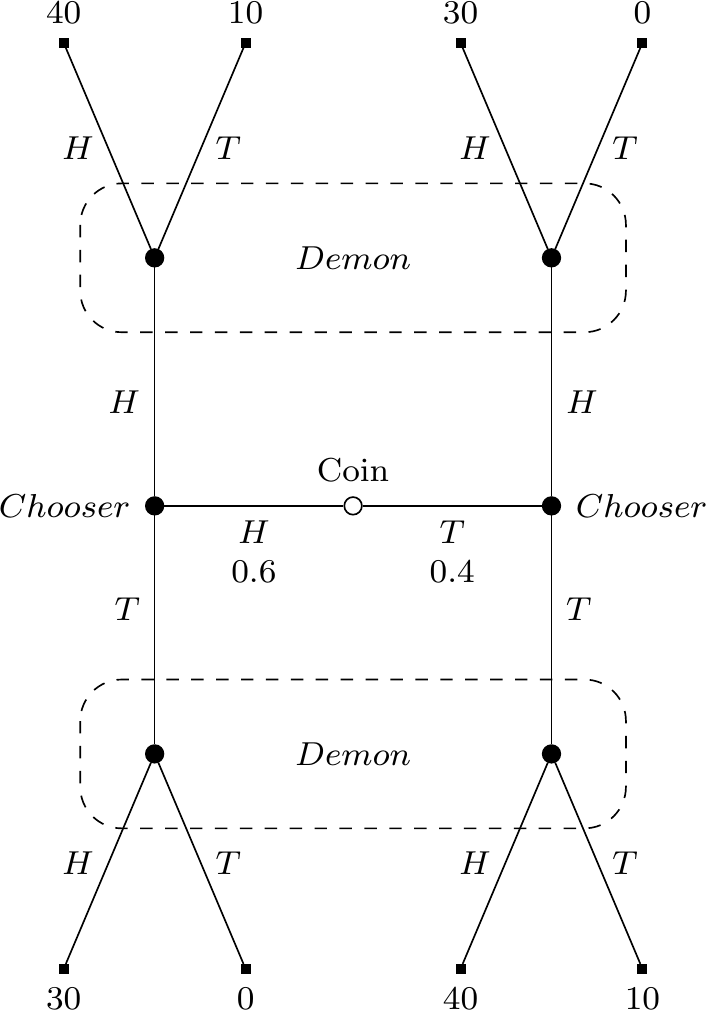
\includegraphics{substantive_files/figure-pdf/fig-cho-kreps-1.png}

}

\caption{\label{fig-cho-kreps}Tree diagram of the beer-quiche game.}

\end{figure}

What will Chooser do? There are two coherent things for Chooser to do,
though each of them is only coherent given a background belief that
isn't entailed by the evidence.

\begin{enumerate}
\def\labelenumi{\arabic{enumi}.}
\tightlist
\item
  Chooser could say Heads however the coin lands. Demon gets no
  information from Chooser, so their probability that the coin landed
  Heads is 0.6, so they will say Heads. Further, Chooser believes that
  if they were to say Tails, Demon would say Tails, so saying Heads
  produces the best expected return even after seeing the coin.
\item
  Chooser could say Tails however the coin lands. Demon gets no
  information from Chooser, so their probability that the coin landed
  Heads is 0.6, so they will say Heads. Further, Chooser believes that
  if they were to say Heads, Demon would say Tails, so saying Tails
  produces the best expected return even after seeing the coin.
\end{enumerate}

While both of these are coherent, there is something very odd, very
unintuitive about option 2. I guess we've been trained to be sceptical
when philosophers report intuitions, but here we have a very large data
pool to draw on. Cho and Kreps reported essentially the same intuition.
Their paper has been cited tens of thousands of times, and I don't think
this intuition has been often questioned. Option 2, while coherent, is
unintuitive. It is the kind of option that the theory of rationality
behind game theory, and behind decision theory, should rule out.

But what about it is incoherent? One might think it is because it has an
expected return of \$34, while option 1 has an expected return of \$36.
But we showed in section Indecisive ref that using expected returns to
choose between coherent options leads to implausible results. Moreover,
if you change the payout in the bottom row to \$50, the intuition
doesn't really go away, but the expected return of option 2 is now \$38;
higher option 1's payout.\footnote{I believe if you change that payout
  to \$65, the various regret based theories I discussed in
  Chapter~\ref{sec-indecisive} also start preferring option 2. But
  applying these theories to complex cases is hard, so I'm not quite
  sure about this.} Alternatively, one might think it is because option
2 requires Chooser to believe a counterfactual that is not entailed by
the evidence. But option 1 also requires Chooser to believe a
counterfactual that is not entailed by the evidence. That can't be the
difference between them, but it is closer to the truth.

What Cho and Kreps argue, persuasively, is that the difference between
the options is that in one case the counterfactual belief is reasonable,
and in the other it is unreasonable. Assume Chooser plans to adopt
option 1. But when it becomes time to play, they change their mind, and
say Tails. What would explain that? Not the coin landing Heads - given
their plan, they will get the maximum possible payout by sticking to the
plan (assuming Demon has done their job). No, the only plausible
explanation is the coin landed Tails, and Chooser was (foolishly)
chasing the extra \$10. In option 1, Chooser believes the counterfactual
that's grounded in Demon picking an explanation that makes sense. What
about in option 2? Here, everything is back to front. If Chooser is ever
going to depart from their plan, it's when the coin lands Heads. Then
Chooser might chase the extra \$10 by saying Heads. But Chooser has to
believe that were they to depart from the plan, Demon would draw the
explanation that makes no sense whatsoever, that they gave up on their
plan even though it was about to lead to the best possible outcome. This
makes no sense at all. And in fact it makes less sense the more you
increase the payout in line 8.

So that's why decision theory requires substantive rationality. The
right decision theory should say to take option 1. And the argument
against option 2 is not that it is incoherent, but that carrying it out
requires believing Demon will do things that make no sense given Demon's
evidence. It is substantive, not structural, rationality that rules out
option 2. And yet, as the game theorists have insisted, option 2 must be
ruled out. So decision theory should be sensitive to substantial
rationality.

\bookmarksetup{startatroot}

\hypertarget{sec-weak}{%
\chapter{Weak Dominance, Once}\label{sec-weak}}

An option \emph{a} weakly dominates another option \emph{b} if \emph{a}
is at least as good as \emph{b} in all states, and better than \emph{b}
in some states. Just what role weak dominance has in decision theory is
one of the most unsettled topics in game theory. There are three natural
positions, and all of them are occupied. One is that weak dominance is
of no significance. A second is that ideal agents do not choose weakly
dominated options, and that's the only role weak dominance has. And a
third is that ideal agents do not choose options that are eliminated by
an iterative process of deleting weakly dominated strategies. I'm going
to argue in favour of the middle position. I'm not going to try to argue
this is the standard game-theoretic move; as I said, I think you can
find prominent support for all three options. To argue for the middle
position requires making two cases: first, that weakly dominated options
are not ideally chosen; and second, that options that would be
eliminated by iterative deletion of weakly dominated options are ideally
chosen. I'll argue for these in turn.

\hypertarget{sec-weak-avoid}{%
\section{Avoid Weakly Dominated Options}\label{sec-weak-avoid}}

Start with Table~\ref{tbl-first-wd}; what would the ideal chooser do?

\hypertarget{tbl-first-wd}{}
\begin{longtable}[]{@{}ccc@{}}
\caption{\label{tbl-first-wd}A ratifiable, weakly dominated,
option.}\tabularnewline
\toprule\noalign{}
& PU & PD \\
\midrule\noalign{}
\endfirsthead
\toprule\noalign{}
& PU & PD \\
\midrule\noalign{}
\endhead
\bottomrule\noalign{}
\endlastfoot
\textbf{U} & 1 & 1 \\
\textbf{D} & 0 & 1 \\
\end{longtable}

On the one hand, D is ratifiable, as long as Demon is sufficiently
reliable. If Demon will in fact get the predictions right, D gets a
return of 1, and had Chooser played U, they would have still received 1.
So they would not regret playing D, so by ratifiability it is fine to
play it. Against this, there are three reasons to not play D.

First, it is rather unrealistic to think that the probability that Demon
will make an accurate prediction is 1. And even if Demon's prediction is
correct with probability 1 - ε, then D will not be ratifiable. I'm
inclined to rule out, on broadly Humean grounds, the very possibility of
a Demon whose predictions are correct with probability 1, but is
causally independent of Chooser's choice. Temporally backwards causation
is not a logical impossibility, and a world where the predictions are
correct with probability 1 seems like a world which has backwards
causation. I don't want to rest the case for GDT on contentious
metaphysics, so I won't lean on this point.

Second, playing D involves taking on an uncompensated risk. It might be
that we don't have a good way of capturing within probability theory
just what this risk is. Perhaps you think that it makes sense to say
that Demon is correct with probability 1. Still, in some sense D has a
risk of failure that U lacks. One should not take on a risk without some
compensation. So one should not play D in this case. This, I think, is
the most persuasive argument against D.\footnote{This paragraph is
  somewhere between heavily influence by, and a notational variant on,
  the argument in section 3 of Stalnaker
  (\protect\hyperlink{ref-Stalnaker1999}{1999}).}

Third, it has been argued by game theorists that we should always allow
for the possibility that one or other player in a game will make some
kind of performance error. This idea is at the heart of Reinhard
Selten's notion of trembling hand equilibrium
(\protect\hyperlink{ref-Selten1975}{Selten 1975}), and Roger Myerson's
notion of proper equilibrium
(\protect\hyperlink{ref-Myerson1978}{Myerson 1978}). If a strategy would
not make sense if the probability of an error by one or other player was
positive, even if it was arbitrarily low, it should not be played. Since
D only makes sense if the probability of an error by Demon is 0, that
means D should not be played.

\hypertarget{sec-weak-iterate}{%
\section{Against Iterative Deletion}\label{sec-weak-iterate}}

If it is good to remove weakly dominated options, then one might think
it follows straight away that it is good to keep doing this.\footnote{This
  suggestion is made by, for example Hare and Hedden
  (\protect\hyperlink{ref-HareHedden2015}{2015}).} Think about
Table~\ref{tbl-wd-itd}.

\hypertarget{tbl-wd-itd}{}
\begin{longtable}[]{@{}cccc@{}}
\caption{\label{tbl-wd-itd}An example of iterated weak
dominance.}\tabularnewline
\toprule\noalign{}
& PU & PD & PX \\
\midrule\noalign{}
\endfirsthead
\toprule\noalign{}
& PU & PD & PX \\
\midrule\noalign{}
\endhead
\bottomrule\noalign{}
\endlastfoot
\textbf{U} & 1 & 1 & 0 \\
\textbf{D} & 0 & 1 & 1 \\
\textbf{X} & 0 & 0 & 1 \\
\end{longtable}

In Table~\ref{tbl-wd-itd}, X is weakly dominated by D. So it shouldn't
be played. But if X isn't played, then PX is weakly dominated by both PU
and PD. Demon can't make a correct prediction by playing PX, since by
hypothesis it won't be played, so it can't be better than PU or PD. But
both PU and PD can be better than PX. So PX is now weakly dominated. So
let's remove it as well. If both X and PX are deleted, we're back to
Table~\ref{tbl-first-wd}, in which we said Chooser should play U.

So does it make sense to say that U is the only play in
Table~\ref{tbl-wd-itd}? I think not, for three reasons.

First, as Bonanno (\protect\hyperlink{ref-Bonanno2018}{2018, 37}) points
out, in general iterative deletion of weakly dominated strategies is not
a well defined decision procedure. It turns out that in two player
games, the order that weakly dominated strategies are deleted can affect
which choices one ends up with. There are ways of fixing this problem,
by specifying one or other order of deletion as canonical, but they all
feel somewhat artificial.

Second, the reasons we gave for avoiding the weakly dominated option in
Table~\ref{tbl-first-wd} simply don't carry over to
Table~\ref{tbl-wd-itd}. In the latter game, D is not an uncompensated
risk. It's true that D loses if Demon makes an incorrect prediction and
plays PU. But U loses if Demon makes an incorrect prediction and plays
PX. Unless one thinks that PX is particularly unlikely to be played, it
seems U and D are just as risky as each other. So both of them look like
rational plays.

Third, iterative deletion of weakly dominated strategies (combined with
the \protect\hyperlink{sec-dual}{dual mandate} approach to dynamic
choice) leads to a single solution to the
\protect\hyperlink{tbl-money-burning}{money burning game} described by
Ben-Porath and Dekel (\protect\hyperlink{ref-BenPorathDekel1992}{1992}).
The money burning game has two players, and two stages. At stage 1,
Column will have the choice to burn or not burn \$20. The burning will
be public, so Row will see what Column does, or does not do. At stage 2,
Row and Column will play the simultaneous move game in
Table~\ref{tbl-money-burning-part-two}.

\hypertarget{tbl-money-burning-part-two}{}
\begin{longtable}[]{@{}ccc@{}}
\caption{\label{tbl-money-burning-part-two}The second stage of the money
burning game}\tabularnewline
\toprule\noalign{}
& A & B \\
\midrule\noalign{}
\endfirsthead
\toprule\noalign{}
& A & B \\
\midrule\noalign{}
\endhead
\bottomrule\noalign{}
\endlastfoot
\textbf{A} & \$10, \$40 & \$0, \$0 \\
\textbf{B} & \$0, \$0 & \$40, \$10 \\
\end{longtable}

Here is one way to think about the game. I'm going to number the steps
here so we can refer back to them later.

\begin{enumerate}
\def\labelenumi{\arabic{enumi}.}
\tightlist
\item
  It would be irrational to burn the money and play B, since that
  results in a maximum possible payout to Column of -\$10, when any
  strategy that involves not burning the money results in a minimum
  payout of \$0.
\item
  So Row can infer that if Column burns the money, they are playing A.
  So if Column burns the money, Row would maximise their own return by
  also playing A.
\item
  Since Column can figure out everything in steps 1-2, it follows that
  burning the money will get them a return of \$20, while playing B gets
  at most \$10, so it is irrational to ever play B.
\item
  Since Row can figure out steps 1-3, it follows that Row knows that
  Column will play A, hence it is always rational for Row to play A.
\item
  Hence Column does not need to burn the money, since Row will play A,
  and hence playing A without burning will get them \$40.
\end{enumerate}

So this looks like an interesting result. By just giving Column the
option of burning the money, we guarantee that Column will get their
best possible outcome, even though they don't actually use that option.
We'll come back to whether this reasoning works. (Spoiler alert: I'm
going to endorse an existing objection to it.)

Let's look at the argument in something like strategic form. For
simplicity, I'm going to assume Column has four strategies: whether to
burn or not burn, crossed with whether to play A or B in
Table~\ref{tbl-money-burning-part-two}. Strictly speaking, we should
distinguish strategies that differ in what Column is disposed to do in
the non-taken option at stage 1, but such distinctions don't matter to
the analysis, and end up cluttering the table. Row has four strategies:
two choices for what to do if Column burns the money, crossed with two
choices for what to do if Column keeps the money.

So as not to confuse the Burning with playing option B, I'll write
\textbf{L} for Lighting the money on fire, and \textbf{K} for Keeping
the money. So Column's strategies will be one of L and K, followed by
one of A and B. For Row, I'll write XY for the strategy of doing option
X if Column keeps the money, and option Y if Column lights it on fire.
So AB is the strategy of doing A iff they don't see the money on fire.
Given that, here is the payout table. (To reduce clutter, I'll write the
payouts in dollars, but will leave off the dollar signs.)

\hypertarget{tbl-money-burning}{}
\begin{longtable}[]{@{}ccccc@{}}
\caption{\label{tbl-money-burning}Simplified strategic form of the money
burning game.}\tabularnewline
\toprule\noalign{}
& KA & KB & LA & LB \\
\midrule\noalign{}
\endfirsthead
\toprule\noalign{}
& KA & KB & LA & LB \\
\midrule\noalign{}
\endhead
\bottomrule\noalign{}
\endlastfoot
\textbf{AA} & 10, 40 & 0, 0 & 10, 20 & 0, -20 \\
\textbf{AB} & 10, 40 & 0, 0 & 0, -20 & 40, -10 \\
\textbf{BA} & 0, 0 & 40, 10 & 10, 20 & 0, -20 \\
\textbf{BB} & 0, 0 & 40, 10 & 0, -20 & 10, -10 \\
\end{longtable}

We can use weak dominance to then reason as follows.

\begin{enumerate}
\def\labelenumi{\arabic{enumi}.}
\tightlist
\item
  LB is strongly dominated by both KA and KB, so it won't be played.
\item
  If LB is deleted, then AB is weakly dominated by AA, and BB is weakly
  dominated by BA, so both AB and BB can be deleted.
\item
  Without AB and BB, LA strongly dominates KB, so KB can be deleted.
\item
  Without KB and LB, AA weakly dominates BA, so BA can be deleted.
\item
  Without AB, BA and BB, KA strongly dominates LA, so LA can be deleted.
\end{enumerate}

The result is that only AA and KA remain, and that's the solution to the
game. Note that it's not just that we've got the same result by thinking
through the strategic form of the game as we'd reached by the earlier
dynamic analysis, we've reached it in exactly the same way. Whatever one
thinks in general about strategic analysis of dynamic games, in this
case it seems the two analyses are as good as each other.

That's bad news for iterated weak dominance, because in the dynamic
argument, step 2 is bad. That implies that in the strategic argument,
which uses weak dominance, step 2 is also bad. Notably, that's the very
first step where iterated weak dominance is used, so we have strong
evidence that iterated weak dominance is the culprit here.

The problem with step 2, as Stalnaker
(\protect\hyperlink{ref-Stalnaker1998}{1998}) points out, is that it
confuses indicative and subjunctive conditionals. What Row knows at that
point is the negation of a conjunction: it's not the case that Column
will burn the money and play B. Arguably, that implies the indicative
conditional: If Column burns the money, they don't play B. But what is
needed for the next step is the subjunctive: If Column burned the money,
they would not play B. And that doesn't at all follow from the negated
conjunction.

Maybe you don't agree that a subjunctive conditional is what Row needs
this point. That part of Stalnaker's analysis is unnecessary for the
main argument. It's enough to note that this negated conjunction can't
be enough to derive any inferences about what to do if Column burns the
money. That's because by the end of the derivation, Row knows that
column (if rational) won't burn the money. So here's another negated
conjunction that they know: it's not the case that Column will burn the
money and play A. They know this because they know the first conjunct is
false, and they are (on standard assumptions) logically omniscient.
Since Row's knowledge is symmetric in this respect, they know both the
negated conjunctions, Column won't burn and play A, and, Column won't
burn and play B, knowledge of one of them can't motivate an asymmetric
attitude to what Column will do.

The five-step argument is self-undermining in a related way. It
concludes that if Column is rational they won't burn the money. But it
gets there by making substantive inferences about what Column will do if
they rationally burn the money. There are no such substantive inferences
to draw; rational Column will (according to the argument) not burn the
money, so once Row sees the money on fire, they should infer Column is
irrational, and stop making any inferences about what Column will or
won't do based on the assumption of rationality.

From all this, I conclude that iterated weak dominance reasoning rests
on a fallacy. I agree with Stalnaker's diagnosis that the fallacy is
confusing indicative and subjunctive conditionals, but as I've argued in
the last two paragraphs, there is independent reason to accept
Stalnaker's claim that there is a fallacy involved even if you don't
accept his diagnosis.

\hypertarget{sec-weak-strong}{%
\section{Back to Strong Dominance}\label{sec-weak-strong}}

This argument might, for some readers, trigger guilt by association
concerns. If initially appealing reasoning like the 1-5 inference in
Section~\ref{sec-weak-iterate} is wrong, might it also be that iterated
strong dominance reasoning rests on a fallacy?

I suspect that concern is at least half-right; some informal
presentations of iterated strong dominance reasoning probably does
commit exactly the same fallacy. But it turns out not to matter; we have
independent reason to accept iterated strong dominance

The reason comes from the theorem of Pearce's that I mentioned back in
Section~\ref{sec-no-ratify}, in the context of discussing
\protect\hyperlink{tbl-frustrator}{The Frustrator}. Pearce goes on to
show something stronger than what I described there, but it needs a
little more terminology to state it.

Say a strategy \emph{S} in a two player game is a
best-response\textsubscript{1} iff there is some probability
distribution \emph{Pr} over the other player's strategies such that
given \emph{Pr}, no strategy available to the player has a higher
expected return than \emph{S} does.

Say a strategy \emph{S} in a two player game is a
best-response\textsubscript{\emph{k}+1} iff there is some probability
distribution \emph{Pr} over the other player's strategies such that (a)
\emph{Pr} only assigns positive probability to the other player choosing
strategies which are best-responses\textsubscript{\emph{k}}, and (b)
given \emph{Pr}, no strategy available to the player has a higher
expected return than \emph{S} does.

Finally, say that a strategy \emph{S} is \textbf{rationalisable} iff for
any \emph{n}, it is a best-response\textsubscript{\emph{k}}.

It is very intuitive that given common knowledge of rationality, each
player should play rationalisable strategies. Playing rationalisable
strategies just means having answers to all of the following questions.

\begin{itemize}
\tightlist
\item
  Why are you playing \emph{S}? Because my credence distribution over
  the other player's strategies is \emph{Pr}\textsubscript{0}, and given
  \emph{Pr}\textsubscript{0}, \emph{S} maximises expected returns.
\item
  Why is your credence distribution over the other player's strategies
  \emph{Pr}\textsubscript{0}? Because for every strategy that
  \emph{Pr}\textsubscript{0} gives positive probability to, there is
  some probability distribution \emph{Pr}\textsubscript{1} that they
  might have over my strategies such that, given
  \emph{Pr}\textsubscript{1}, that strategy is optimal.
\item
  Why should we think \emph{Pr}\textsubscript{1} is their probability
  distribution? Because for every strategy of mine that
  \emph{Pr}\textsubscript{1} gives positive probability to, there is
  some probability distribution \emph{Pr}\textsubscript{2} such that
  that strategy is optimal given \emph{Pr}\textsubscript{2}.
\end{itemize}

This line of questioning could go on indefinitely. Presumably
\emph{Pr}\textsubscript{2} isn't defined over any old things the other
player might play. But if the original strategy is rationalisable, it
will give positive probabilities to things that it would make some sense
for the other player to play. And so on indefinitely.

This, ultimately, is why I think dominance reasoning, and in particular
iterated dominance reasoning, should be incorporated into our decision
theory. Using dominance reasoning is a somewhat convenient shorthand for
what we should be doing, namely finding rationalisable strategies.

To be sure, I think we should do somewhat more than find rationalisable
strategies. We should also find strategies that are not weakly dominated
(as argued in Chapter~\ref{sec-weak}), and which are substantively
rational (as argued in Chapter~\ref{sec-substantive}). But the first
necessary step is to remove the non-rationalisable strategies.

\hypertarget{sec-weak-summary}{%
\section{Summary}\label{sec-weak-summary}}

So I conclude that we just need one round of deleting weakly dominated
options to get rid of irrational plays. D is irrational in
Table~\ref{tbl-first-wd}, but not in Table~\ref{tbl-wd-itd}. The reasons
for not iterating weak dominance reasoning do not apply to strong
dominance reasoning, and iterated strong dominance reasoning leads to
the same results as reasoning that is unimpeachable, namely finding
rationalisable strategies.

\bookmarksetup{startatroot}

\hypertarget{sec-conclusion}{%
\chapter{Conclusion}\label{sec-conclusion}}

Given all that, here is the positive theory, what I'm calling Gamified
Decision Theory (GDT). The core is that rational choices are ratifiable.
That is, they maximise expected utility from the perspective of someone
who chooses them. Formally, that means that in a particular problem,
with choices \emph{o}\textsubscript{1}, \(\dots\),
\emph{o\textsubscript{m}}, and causally independent states
\emph{s}\textsubscript{1}, \(\dots\) \emph{s\textsubscript{n}}, a choice
\emph{o} is rational iff there is some probability function Pr that is a
rational credal distribution over the \emph{s} after choosing \emph{o},
and such that for all \emph{o\textsubscript{j}},
\(\Sigma\)Pr(\emph{s\textsubscript{i}})V(\emph{os\textsubscript{i}}) ≥
\(\Sigma\)Pr(\emph{s\textsubscript{i}})V(\emph{o\textsubscript{j}s\textsubscript{i}}).

There are two extra clauses. First, \emph{o} is choiceworthy only if it
is not be weakly dominated by any other option. Second, if one is making
a series of decisions in a tree, and one knows that one will be rational
and not change one's preferences throughout, then both the decisions one
makes at any given time, and the set of decisions one collectively
makes, must satisfy all the other conditions of rational choice. That
is, they must be ratifiable and not weakly dominated.

The big advantage of this theory is that it satisfies the nine
conditions I mentioned at the start, and that it is consistent with Exit
Principle. These turn out to be very sharp constraints on a theory. For
example, any theory that associates some number with each choice, and
says to maximise the number, will violate the Indecisiveness constraint.
Any theory that simply the chooser's credences as given will violate the
Substantiveness constraint. The vast bulk of decision theories on the
market in philosophy do at least one of these two things, and typically
both. So we have strong reason to prefer GDT to them.

GDT does require that mixed strategies are available to choosers, on
pain of saying that a lot of decision problems are dilemmas. That is not
a problem for GDT, since ideal agents can perform mixed strategies. It
is a shortcoming to not be able to perform them, and ideal agents don't
have these kinds of shortcomings. But it does suggest an important
research program in working out how GDT should be altered for agents who
lack one or other idealisation. In fact it suggests two research
programs: a descriptive one, setting out what choosers who don't satisfy
one or other idealisation in fact do; and a normative one, setting out
what these choosers should do. But those projects are for a very
different paper.\footnote{Thanks to many people for conversations on
  these topics, especially Dmitri Gallow and Ishani Maitra, and
  audiences and ACU and UBC, and students in my group choices classes at
  University of Michigan.}

\bookmarksetup{startatroot}

\hypertarget{references}{%
\chapter*{References}\label{references}}
\addcontentsline{toc}{chapter}{References}

\markboth{References}{References}

\hypertarget{refs}{}
\begin{CSLReferences}{1}{0}
\leavevmode\vadjust pre{\hypertarget{ref-Ahmed2012}{}}%
Ahmed, Arif. 2012. {``Push the Button.''} \emph{Philosophy of Science}
79 (3): 386--95. \url{https://doi.org/10.1086/666065}.

\leavevmode\vadjust pre{\hypertarget{ref-Ahmed2014a}{}}%
---------. 2014. {``Dicing with Death.''} \emph{Analysis} 74 (4):
587--92. \url{https://doi.org/10.1093/analys/anu084}.

\leavevmode\vadjust pre{\hypertarget{ref-Ahmed2020}{}}%
---------. 2020. {``Equal Opportunities in Newcomb's Problem and
Elsewhere.''} \emph{Mind} 129 (515): 867--86.
\url{https://doi.org/10.1093/mind/fzz073}.

\leavevmode\vadjust pre{\hypertarget{ref-Akerlof1970}{}}%
Akerlof, George. 1970. {``The Market for "Lemons": Quality Uncertainty
and the Market Mechanism.''} \emph{Quarterly Journal of Economics} 84
(3): 488--500. \url{https://doi.org/10.2307/1879431}.

\leavevmode\vadjust pre{\hypertarget{ref-Alcoba2023}{}}%
Alcoba, Natalie. 2023. {``In Argentina, Inflation Passes 100\% (and the
Restaurants Are Packed).''} \emph{The New York Times}, June 19, 2023.
\url{https://www.nytimes.com/2023/06/19/world/americas/argentina-inflation-peso-restaurants.html}.

\leavevmode\vadjust pre{\hypertarget{ref-Allais1953}{}}%
Allais, M. 1953. {``Le Comportement de l'homme Rationnel Devant Le
Risque: Critique Des Postulats Et Axiomes de l'ecole Americaine.''}
\emph{Econometrica} 21 (4): 503--46.
\url{https://doi.org/10.2307/1907921}.

\leavevmode\vadjust pre{\hypertarget{ref-Arntzenius2008}{}}%
Arntzenius, Frank. 2008. {``No Regrets; or, Edith Piaf Revamps Decision
Theory.''} \emph{Erkenntnis} 68 (2): 277--97.
\url{https://doi.org/10.1007/s10670-007-9084-8}.

\leavevmode\vadjust pre{\hypertarget{ref-Barnett2022}{}}%
Barnett, David James. 2022. {``Graded Ratifiability.''} \emph{Journal of
Philosophy} 119 (2): 57--88.
\url{https://doi.org/10.5840/jphil202211925}.

\leavevmode\vadjust pre{\hypertarget{ref-BenPorathDekel1992}{}}%
Ben-Porath, Elchanan, and Eddie Dekel. 1992. {``Signaling Future Actions
and the Potential for Sacrifice.''} \emph{Journal of Economic Theory} 57
(1): 36--51. \url{https://doi.org/10.1016/S0022-0531(05)80039-0}.

\leavevmode\vadjust pre{\hypertarget{ref-Blackwell1951}{}}%
Blackwell, David. 1951. {``Comparison of Experiments.''}
\emph{Proceedings of the Berkeley Symposium on Mathematical Statistics
and Probability} 2 (1): 93--102.

\leavevmode\vadjust pre{\hypertarget{ref-Bonanno2018}{}}%
Bonanno, Giacomo. 2018. {``Game Theory.''} Davis, CA: Kindle Direct
Publishing. 2018.
\url{http://faculty.econ.ucdavis.edu/faculty/bonanno/GT_Book.html}.

\leavevmode\vadjust pre{\hypertarget{ref-BottomleyWilliamsonnd}{}}%
Bottomley, Christopher, and Timothy Luke WIlliamson. n.d. {``Rational
Risk-Aversion: Good Things Come to Those Who Weight.''} {P}hilosophy and
{P}henomenological {R}esearch.
\url{https://doi.org/doi.org/10.1111/phpr.13006}.

\leavevmode\vadjust pre{\hypertarget{ref-BuchakRisk}{}}%
Buchak, Lara. 2013. \emph{Risk and Rationality}. Oxford: Oxford
University Press.

\leavevmode\vadjust pre{\hypertarget{ref-Buchak2017}{}}%
---------. 2017. {``Pr{é}cis of Risk and Rationality.''}
\emph{Philosophical Studies} 174 (9): 2363--68.
\url{https://doi.org/10.1007/s11098-017-0904-7}.

\leavevmode\vadjust pre{\hypertarget{ref-Callahan2021}{}}%
Callahan, Laura Frances. 2021. {``Epistemic Existentialism.''}
\emph{Episteme} 18 (4): 539--54.
\url{https://doi.org/10.1017/epi.2019.25}.

\leavevmode\vadjust pre{\hypertarget{ref-ChandlerSEP}{}}%
Chandler, Jake. 2017. {``{Descriptive Decision Theory}.''} In \emph{The
{Stanford} Encyclopedia of Philosophy}, edited by Edward N. Zalta,
{W}inter 2017.
\url{https://plato.stanford.edu/archives/win2017/entries/decision-theory-descriptive/};
Metaphysics Research Lab, Stanford University.

\leavevmode\vadjust pre{\hypertarget{ref-Chang2002}{}}%
Chang, Ruth. 2002. {``The Possibility of Parity.''} \emph{Ethics} 112
(4): 659--88. \url{https://doi.org/10.1086/339673}.

\leavevmode\vadjust pre{\hypertarget{ref-Chernoff1954}{}}%
Chernoff, Herman. 1954. {``Rational Selection of Decision Functions.''}
\emph{Econometrica} 22 (4): 422--43.
\url{https://doi.org/10.2307/1907435}.

\leavevmode\vadjust pre{\hypertarget{ref-ChoKreps1987}{}}%
Cho, In-Koo, and David M. Kreps. 1987. {``Signalling Games and Stable
Equilibria.''} \emph{The Quarterly Journal of Economics} 102 (2):
179--221. \url{https://doi.org/10.2307/1885060}.

\leavevmode\vadjust pre{\hypertarget{ref-cohen2023sequential}{}}%
Cohen, Shani, and Shengwu Li. 2023. {``Sequential Cursed Equilibrium.''}
\url{https://arxiv.org/abs/2212.06025}.

\leavevmode\vadjust pre{\hypertarget{ref-Cohen2013}{}}%
Cohen, Stewart. 2013. {``A Defence of the (Almost) Equal Weight View.''}
In \emph{The Epistemology of Disagreement: New Essays}, edited by David
Christensen and Jennifer Lackey, 98--117. Oxford: Oxford University
Press.

\leavevmode\vadjust pre{\hypertarget{ref-Conlisk1996}{}}%
Conlisk, John. 1996. {``Why Bounded Rationality?''} \emph{Journal of
Economic Literature} 34 (2): 669--700.

\leavevmode\vadjust pre{\hypertarget{ref-Das2023}{}}%
Das, Nilanjan. 2023. {``The Value of Biased Information.''}
\emph{British Journal for the Philosophy of Science} 74 (1): 25--55.
\url{https://doi.org/10.1093/bjps/axaa003}.

\leavevmode\vadjust pre{\hypertarget{ref-Davey2011}{}}%
Davey, Kevin. 2011. {``Idealizations and Contextualism in Physics.''}
\emph{Philosophy of Science} 78 (1): 16--38.
\url{https://doi.org/10.1086/658093}.

\leavevmode\vadjust pre{\hypertarget{ref-Dogramaci2012}{}}%
Dogramaci, Sinan. 2012. {``Reverse Engineering Epistemic Evaluations.''}
\emph{Philosophy and Phenomenological Research} 84 (3): 513--30.
\url{https://doi.org/10.1111/j.1933-1592.2011.00566.x}.

\leavevmode\vadjust pre{\hypertarget{ref-Egan2007}{}}%
Egan, Andy. 2007a. {``Some Counterexamples to Causal Decision Theory.''}
\emph{Philosophical Review} 116 (1): 93--114.
\url{https://doi.org/10.1215/00318108-2006-023}.

\leavevmode\vadjust pre{\hypertarget{ref-Egan2007-EGASCT}{}}%
---------. 2007b. {``{Some Counterexamples to Causal Decision
Theory}.''} \emph{Philosophical Review} 116 (1): 93--114.
\url{https://doi.org/10.1215/00318108-2006-023}.

\leavevmode\vadjust pre{\hypertarget{ref-Elga2000}{}}%
Elga, Adam. 2000. {``Self-Locating Belief and the Sleeping Beauty
Problem.''} \emph{Analysis} 60 (4): 143--47.
\url{https://doi.org/10.1093/analys/60.2.143}.

\leavevmode\vadjust pre{\hypertarget{ref-Elliot2019}{}}%
Elliott, Edward. 2019. {``Normative Decision Theory.''} \emph{Analysis}
79 (4): 755--72. \url{https://doi.org/10.1093/analys/anz059}.

\leavevmode\vadjust pre{\hypertarget{ref-EysterRabin2005}{}}%
Eyster, Erik, and Matthew Rabin. 2005. {``Cursed Equilibrium.''}
\emph{Econometrica} 73 (5): 1623--72.
\href{https://10.1111/j.1468-0262.2005.00631.x}{10.1111/j.1468-0262.2005.00631.x}.

\leavevmode\vadjust pre{\hypertarget{ref-Fey2012}{}}%
Fey, Mark. 2012. {``Symmetric Games with Only Asymmetric Equilibria.''}
\emph{Games and Economic Behavior} 75 (1): 424--27.
\url{https://doi.org/10.1016/j.geb.2011.09.008}.

\leavevmode\vadjust pre{\hypertarget{ref-fong2023cursed}{}}%
Fong, Meng-Jhang, Po-Hsuan Lin, and Thomas R. Palfrey. 2023. {``Cursed
Sequential Equilibrium.''} \url{https://arxiv.org/abs/2301.11971}.

\leavevmode\vadjust pre{\hypertarget{ref-Fuscond}{}}%
Fusco, Melissa. n.d. {``Absolution of a Causal Decision Theorist.''}
No{û}s. \url{https://doi.org/10.1111/nous.12459}.

\leavevmode\vadjust pre{\hypertarget{ref-Gallow2020}{}}%
Gallow, J. Dmitri. 2020. {``The Causal Decision Theorist's Gudie to
Managing the News.''} \emph{The Journal of Philosophy} 117 (3): 117--49.
\url{https://doi.org/10.5840/jphil202011739}.

\leavevmode\vadjust pre{\hypertarget{ref-Gallownd}{}}%
---------. n.d. {``The Sure Thing Principle Leads to Instability.''}
Philosophical Quarterly.
\url{https://philpapers.org/archive/GALTST-2.pdf}.

\leavevmode\vadjust pre{\hypertarget{ref-GibbardHarper1978}{}}%
Gibbard, Allan, and William Harper. 1978. {``Counterfactuals and Two
Kinds of Expected Utility.''} In \emph{Foundations and Applications of
Decision Theory}, edited by C. A. Hooker, J. J. Leach, and E. F.
McClennen, 125--62. Dordrecht: Reidel.

\leavevmode\vadjust pre{\hypertarget{ref-Good1967}{}}%
Good, I. J. 1967. {``On the Principle of Total Evidence.''}
\emph{British Journal for the Philosophy of Science} 17 (4): 319--21.
\url{https://doi.org/10.1093/bjps/17.4.319}.

\leavevmode\vadjust pre{\hypertarget{ref-Goodsellnd}{}}%
Goodsell, Zachary. n.d. {``Decision Theory Unbound.''} No{û}s.
\url{https://doi.org/10.1111/nous.12473}.

\leavevmode\vadjust pre{\hypertarget{ref-GrantEtAl2021}{}}%
Grant, Simon, Guerdjikova Ani, and John Quiggin. 2021. {``Ambiguity and
Awareness: A Coherent Multiple Priors Model.''} \emph{The B.E. Journal
of Theoretical Economics} 21 (2): 571--612.
\url{https://doi.org/10.1515/bejte-2018-0185}.

\leavevmode\vadjust pre{\hypertarget{ref-GrecoHedden2016}{}}%
Greco, Daniel, and Brian Hedden. 2016. {``Uniqueness and
Metaepistemology.''} \emph{The Journal of Philosophy} 113 (8): 365--95.
\url{https://doi.org/10.1111/phc3.12318}.

\leavevmode\vadjust pre{\hypertarget{ref-Gustafsson2011}{}}%
Gustafsson, Johan E. 2011. {``A Note in Defence of Ratificationism.''}
\emph{Erkenntnis} 75 (1): 147--50.
\url{https://doi.org/10.1007/s10670-010-9267-6}.

\leavevmode\vadjust pre{\hypertarget{ref-Hammond1988}{}}%
Hammond, Peter J. 1988. {``Consequentialist Foundations for Expected
Utility.''} \emph{Theory and Decision} 25 (1): 25--78.
\url{https://doi.org/10.1007/BF00129168}.

\leavevmode\vadjust pre{\hypertarget{ref-HareHedden2015}{}}%
Hare, Caspar, and Brian Hedden. 2015. {``Self-Reinforcing and
Self-Frustrating Decisions.''} \emph{Noûs} 50 (3): 604--28.
\url{https://doi.org/10.1111/nous.12094}.

\leavevmode\vadjust pre{\hypertarget{ref-Harper1986}{}}%
Harper, William. 1986. {``Mixed Strategies and Ratifiability in Causal
Decision Theory.''} \emph{Erkenntnis} 24 (1): 25--36.
\url{https://doi.org/10.1007/BF00183199}.

\leavevmode\vadjust pre{\hypertarget{ref-Harper1988}{}}%
---------. 1988. {``Causal Decision Theory and Game Theory: A Classic
Argument for Equilibrium Solutions, a Defense of Weak Equilibria, and a
New Problem for the Normal Form Representation.''} In \emph{Causation in
Decision, Belief Change, and Statistics: Proceedings of the Irvine
Conference on Probability and Causation}, edited by William Harper and
Brian Skyrms, 25--48. Dordrecht: Springer Netherlands.
\url{https://doi.org/10.1007/978-94-009-2865-7_2}.

\leavevmode\vadjust pre{\hypertarget{ref-Heinzelmannnd}{}}%
Heinzelmann, Nora. n.d. {``Rationality Is Not Coherence.''}
Philosophical Quarterly. \url{https://doi.org/10.1093/pq/pqac083}.

\leavevmode\vadjust pre{\hypertarget{ref-Horowitz2014}{}}%
Horowitz, Sophie. 2014. {``Immoderately Rational.''} \emph{Philosohical
Studies} 167 (1): 41--56.
\url{https://doi.org/10.1007/s11098-013-0231-6}.

\leavevmode\vadjust pre{\hypertarget{ref-Jackson1998}{}}%
Jackson, Frank. 1998. \emph{From Metaphysics to Ethics: A Defence of
Conceptual Analysis}. Clarendon Press: Oxford.

\leavevmode\vadjust pre{\hypertarget{ref-Jeffrey1983}{}}%
Jeffrey, Richard. 1983. {``Bayesianism with a Human Face.''} In
\emph{Testing Scientific Theories}, edited by J. Earman (ed.).
Minneapolis: University of Minnesota Press.

\leavevmode\vadjust pre{\hypertarget{ref-Joyce2012}{}}%
Joyce, James M. 2012. {``Regret and Instability in Causal Decision
Theory.''} \emph{Synthese} 187 (1): 123--45.
\url{https://doi.org/10.1007/s11229-011-0022-6}.

\leavevmode\vadjust pre{\hypertarget{ref-Keynes1921}{}}%
Keynes, John Maynard. 1921. \emph{Treatise on Probability}. London:
Macmillan.

\leavevmode\vadjust pre{\hypertarget{ref-Keynes1923}{}}%
---------. 1923. \emph{A Tract on Monetary Reform}. London: Macmillan.

\leavevmode\vadjust pre{\hypertarget{ref-Knight1921}{}}%
Knight, Frank. 1921. \emph{Risk, Uncertainty and Profit}. Chicago:
University of Chicago Press.

\leavevmode\vadjust pre{\hypertarget{ref-KopecTitelbaum2016}{}}%
Kopec, Matthew, and Michael G. Titelbaum. 2016. {``The Uniqueness
Thesis.''} \emph{Philosophy Compass} 11 (4): 189--200.
\url{https://doi.org/10.1111/phc3.12318}.

\leavevmode\vadjust pre{\hypertarget{ref-Leend}{}}%
Lee, Wooram. n.d. {``What Is Structural Rationality?''} Philosophical
Quarterly. \url{https://doi.org/10.1093/pq/pqad072}.

\leavevmode\vadjust pre{\hypertarget{ref-LevinsteinSoares2020}{}}%
Levinstein, Benjamin Anders, and Nate Soares. 2020. {``Cheating Death in
Damascus.''} \emph{Journal of Philosophy} 117 (5): 237--66.
\url{https://doi.org/10.5840/jphil2020117516}.

\leavevmode\vadjust pre{\hypertarget{ref-Lewis1969a}{}}%
Lewis, David. 1969. \emph{Convention: A Philosophical Study}. Cambridge:
Harvard University Press.

\leavevmode\vadjust pre{\hypertarget{ref-Lewis1979e}{}}%
---------. 1979. {``Prisoners' Dilemma Is a {N}ewcomb Problem.''}
\emph{Philosophy and Public Affairs} 8 (3): 235--40.

\leavevmode\vadjust pre{\hypertarget{ref-Lewis1981e}{}}%
---------. 1981. {``Why Ain'cha Rich?''} \emph{No{û}s} 15 (3): 377--80.
\url{https://doi.org/10.2307/2215439}.

\leavevmode\vadjust pre{\hypertarget{ref-Lewis1981Mellor}{}}%
---------. 2020a. {``Letter to Hugh Mellor Dated 14 October 1981.''} In
\emph{Philosophical Letters of David k. Lewis}, edited by Helen Beebee
and A. R. J. Fisher, 2: Mind, Language, Epistemology:432--34. Oxford:
Oxford University Press.

\leavevmode\vadjust pre{\hypertarget{ref-Lewis-Gorman-10071979}{}}%
---------. 2020b. {``Letter to Jonathan Gorman, 19 April 1989.''} In
\emph{Philosophical Letters of David {K}. Lewis}, edited by Helen Beebee
and A. R. J. Fisher, 2:472--73. Oxford: Oxford University Press.

\leavevmode\vadjust pre{\hypertarget{ref-LipseyLancaster}{}}%
Lipsey, R. G., and Kelvin Lancaster. 1956. {``The General Theory of
Second Best.''} \emph{Review of Economic Studies} 24 (1): 11--32.
\url{https://doi.org/10.2307/2296233}.

\leavevmode\vadjust pre{\hypertarget{ref-Lota2023}{}}%
Lota, Kenji, and Ulf Hlobil. 2023. {``Resolutions Against Uniqueness.''}
\emph{Erkenntnis} 88 (3): 1013--33.
\url{https://doi.org/10.1007/s10670-021-00391-z}.

\leavevmode\vadjust pre{\hypertarget{ref-McClennen1990}{}}%
McClennan, Edward. 1990b. \emph{Rationality and Dynamic Choice}.
Cambridge: {C}ambridge {U}niversity {P}ress.

\leavevmode\vadjust pre{\hypertarget{ref-McClennan1990}{}}%
---------. 1990a. \emph{Rationality and Dynamic Choice}. Cambridge:
Cambridge University Press.

\leavevmode\vadjust pre{\hypertarget{ref-Meacham2019}{}}%
Meacham, Christopher. 2019. {``Deference and Uniqueness.''}
\emph{Philosohical Studies} 176 (3): 709--32.
\url{https://doi.org/10.1007/s11098-018-1036-4}.

\leavevmode\vadjust pre{\hypertarget{ref-Mills2005}{}}%
Mills, Charles W. 2005. {``"Ideal Theory" as Ideology.''} \emph{Hypatia}
20 (3): 165--84.
\url{https://doi.org/10.1111/j.1527-2001.2005.tb00493.x}.

\leavevmode\vadjust pre{\hypertarget{ref-Moulin1985}{}}%
Moulin, H. 1985. {``Choice Functions over a Finite Set: A Summary.''}
\emph{Social Choice and Welfare} 2 (2): 147--60.

\leavevmode\vadjust pre{\hypertarget{ref-Myerson1978}{}}%
Myerson, R. B. 1978. {``Refinements of the Nash Equilibrium Concept.''}
\emph{International Journal of Game Theory} 7 (2): 73--80.
\url{https://doi.org/10.1007/BF01753236}.

\leavevmode\vadjust pre{\hypertarget{ref-Nash1951}{}}%
Nash, John. 1951. {``Non-Cooperative Games.''} \emph{Annals of
Mathematics} 54 (2): 286--95.

\leavevmode\vadjust pre{\hypertarget{ref-Nozick1969}{}}%
Nozick, Robert. 1969. {``Newcomb's Problem and Two Principles of
Choice.''} In \emph{Essays in Honor of Carl {G}. Hempel: A Tribute on
the Occasion of His Sixty-Fifth Birthday. Hempel: A Tribute on the
Occasion of His Sixty-Fifth Birthday}, edited by Nicholas Rescher,
114--46. Riedel: Springer.

\leavevmode\vadjust pre{\hypertarget{ref-OConnor2019}{}}%
O'Connor, Cailin. 2019. \emph{The Origins of Unfairness: Social
Categories and Cultural Evolution}. Oxford: {O}xford {U}niversity
{P}ress.

\leavevmode\vadjust pre{\hypertarget{ref-Palmira2023}{}}%
Palmira, Michele. 2023. {``Permissivism and the Truth Connection.''}
\emph{Erkenntnis} 88 (2): 641--6556.
\url{https://doi.org/10.1007/s10670-020-00373-7}.

\leavevmode\vadjust pre{\hypertarget{ref-Pearce1984}{}}%
Pearce, David G. 1984. {``Rationalizable Strategic Behavior and the
Problem of Perfection.''} \emph{Econometrica} 52 (4): 1029--50.
\url{https://doi.org/10.2307/1911197}.

\leavevmode\vadjust pre{\hypertarget{ref-Peirce1876}{}}%
Peirce, C. S. 1967. {``Note on the Theory of the Economy of Research.''}
\emph{Operations Research} 15 (4): 643--48.

\leavevmode\vadjust pre{\hypertarget{ref-Podgorski2022}{}}%
Podgorski, Aberlard. 2022. {``Tournament Decision Theory.''}
\emph{No{û}s} 56 (1): 176--203.
\url{https://doi.org/10.1111/nous.12353}.

\leavevmode\vadjust pre{\hypertarget{ref-Quiggin1982}{}}%
Quiggin, John. 1982. {``A Theory of Anticipated Utility.''}
\emph{Journal of Economic Behavior \& Organization} 3 (4): 323--43.
\url{https://doi.org/10.1016/0167-2681(82)90008-7}.

\leavevmode\vadjust pre{\hypertarget{ref-RamseyGeneralProp}{}}%
Ramsey, Frank. 1990. {``General Propositions and Causality.''} In
\emph{Philosophical Papers}, edited by D. H. Mellor, 145--63. Cambridge:
Cambridge University Press.

\leavevmode\vadjust pre{\hypertarget{ref-Richter1984}{}}%
Richter, Reed. 1984. {``Rationality Revisited.''} \emph{Australasian
Journal of Philosophy} 62 (4): 393--404.
\url{https://doi.org/10.1080/00048408412341601}.

\leavevmode\vadjust pre{\hypertarget{ref-Risse2000}{}}%
Risse, Mathias. 2000. {``What Is Rational about Nash Equilibria?''}
\emph{Synthese} 124 (3): 361--84.
\url{https://doi.org/10.1023/a:1005259701040}.

\leavevmode\vadjust pre{\hypertarget{ref-Robinson1949}{}}%
Robinson, Julia. 1949. {``On the Hamiltonian Game (a Traveling Salesman
Problem).''} Santa Monica, CA: The RAND Corporation.

\leavevmode\vadjust pre{\hypertarget{ref-Ross2021}{}}%
Ross, Ryan. 2021. {``Alleged Counterexamples to Uniqueness.''}
\emph{Logos and Episteme} 12 (2): 203--13.

\leavevmode\vadjust pre{\hypertarget{ref-Samuelson1938}{}}%
Samuelson, Paul A. 1938. {``A Note on the Pure Theory of Consumer's
Behaviour.''} \emph{Econometrica} 5 (17): 61--71.
\url{https://doi.org/10.2307/2548836}.

\leavevmode\vadjust pre{\hypertarget{ref-Schrijver2005}{}}%
Schrijver, Alexander. 2005. {``On the History of Combinatorial
Optimization (till 1960).''} \emph{Handbooks in Operations Research and
Management Science} 12: 1--68.
\url{https://doi.org/10.1016/S0927-0507(05)12001-5}.

\leavevmode\vadjust pre{\hypertarget{ref-Schultheis2018}{}}%
Schultheis, Ginger. 2018. {``Living on the Edge: Against Epistemic
Permissivism.''} \emph{Mind} 127 (507): 863--79.
\url{https://doi.org/10.1093/mind/fzw065}.

\leavevmode\vadjust pre{\hypertarget{ref-Selten1975}{}}%
Selten, R. 1975. {``Reexamination of the Perfectness Concept for
Equilibrium Points in Extensive Games.''} \emph{International Journal of
Game Theory} 4 (1): 25--55. \url{https://doi.org/10.1007/BF01766400}.

\leavevmode\vadjust pre{\hypertarget{ref-Sen1971}{}}%
Sen, Amartya. 1971. {``Choice Functions and Revealed Preference.''}
\emph{Review of Economic Studies} 38 (3): 307--17.
\url{https://doi.org/10.2307/2296384}.

\leavevmode\vadjust pre{\hypertarget{ref-Sen2006}{}}%
---------. 2006. {``What Do We Want from a Theory of Justice?''}
\emph{Journal of Philosophy} 103 (5): 215--38.
\url{https://doi.org/10.5840/jphil2006103517}.

\leavevmode\vadjust pre{\hypertarget{ref-Shafer1976}{}}%
Shafer, Glenn. 1976. \emph{A Mathematical Theory of Evidence}.
Princeton: Princeton University Press.

\leavevmode\vadjust pre{\hypertarget{ref-Skyrms1984}{}}%
Skyrms, Brian. 1984. \emph{Pragmatics and Empiricism}. New Haven, CT:
Yale University Press.

\leavevmode\vadjust pre{\hypertarget{ref-Skyrms2004}{}}%
---------. 2004. \emph{The Stag Hunt and the Evolution of Social
Structure}. Cambridge: {C}ambridge {U}niversity {P}ress.

\leavevmode\vadjust pre{\hypertarget{ref-Smullyan1978}{}}%
Smullyan, Raymond. 1978. \emph{What Is the Name of This Book? The Riddle
of Dracula and Other Logical Puzzles}. Englewood Cliffs, NJ:
Prentice-Hall.

\leavevmode\vadjust pre{\hypertarget{ref-Spencer2021b}{}}%
Spencer, Jack. 2021. {``Rational Monism and Rational Pluralism.''}
\emph{Philosophical Studies} 178: 1769--1800.
\url{https://doi.org/10.1007/s11098-020-01509-9}.

\leavevmode\vadjust pre{\hypertarget{ref-Spencer2023}{}}%
---------. 2023. {``Can It Be Irrational to Knowingly Choose the
Best?''} \emph{Australasian Journal of Philosophy} 101 (1): 128--39.
\url{https://doi.org/10.1080/00048402.2021.1958880}.

\leavevmode\vadjust pre{\hypertarget{ref-SpencerWells2019}{}}%
Spencer, Jack, and Ian Wells. 2019. {``Why Take Both Boxes?''}
\emph{{P}hilosophy and {P}henomenological {R}esearch} 99 (1): 27--48.
\url{https://doi.org/10.1111/phpr.12466}.

\leavevmode\vadjust pre{\hypertarget{ref-Stalnaker1998}{}}%
Stalnaker, Robert. 1998. {``Belief Revision in Games: Forward and
Backward Induction.''} \emph{Mathematical Social Sciences} 36 (1):
31--56. \url{https://doi.org/10.1016/S0165-4896(98)00007-9}.

\leavevmode\vadjust pre{\hypertarget{ref-Stalnaker1999}{}}%
---------. 1999. {``Extensive and Strategic Forms: Games and Models for
Games.''} \emph{Research in Economics} 53 (3): 293--319.
\url{https://doi.org/10.1006/reec.1999.0200}.

\leavevmode\vadjust pre{\hypertarget{ref-Stalnaker2008}{}}%
---------. 2008. \emph{Our Knowledge of the Internal World}. Oxford:
Oxford University Press.

\leavevmode\vadjust pre{\hypertarget{ref-Strevens2008}{}}%
Strevens, Michael. 2008. \emph{Depth: An Account of Scientific
Explanations}. Cambridge, MA: Harvard University Press.

\leavevmode\vadjust pre{\hypertarget{ref-Sutton2000}{}}%
Sutton, John. 2000. \emph{Marshall's Tendencies: What Can Economists
Know?} Cambridge, MA: {MIT} Press.

\leavevmode\vadjust pre{\hypertarget{ref-Thoma2019}{}}%
Thoma, Johanna. 2019. {``Risk Aversion and the Long Run.''}
\emph{Ethics} 129 (2): 230--53. \url{https://doi.org/10.1086/699256}.

\leavevmode\vadjust pre{\hypertarget{ref-Valentini2012}{}}%
Valentini, Laura. 2012. {``Ideal Vs. Non-Ideal Theory: A Conceptual
Map.''} \emph{Philosophy Compass} 7 (9): 654--64.
\url{https://doi.org/10.1111/phco.2012.7.issue-9}.

\leavevmode\vadjust pre{\hypertarget{ref-Weatherson2019}{}}%
Weatherson, Brian. 2019. \emph{Normative Externalism}. Oxford: Oxford
University Press.

\leavevmode\vadjust pre{\hypertarget{ref-Wedgwood2012}{}}%
Wedgwood, Ralph. 2012. {``Justified Inference.''} \emph{Synthese} 189
(2): 273--95. \url{https://doi.org/10.1007/s11229-011-0012-8}.

\leavevmode\vadjust pre{\hypertarget{ref-Wedgwood2013a}{}}%
---------. 2013. {``Gandalf's Solution to the Newcomb Problem.''}
\emph{Synthese} 190 (14): 2643--75.
\url{https://doi.org/10.1007/s11229-011-9900-1}.

\leavevmode\vadjust pre{\hypertarget{ref-Weirich1985}{}}%
Weirich, Paul. 1985. {``Decision Instability.''} \emph{Australasian
Journal of Philosophy} 63 (4): 465--72.
\url{https://doi.org/10.1080/00048408512342061}.

\leavevmode\vadjust pre{\hypertarget{ref-Wells2019}{}}%
Wells, Ian. 2019. {``Equal Opportunity and Newcomb's Problem.''}
\emph{Mind} 128 (510): 429--57.
\url{https://doi.org/10.1093/mind/fzx018}.

\leavevmode\vadjust pre{\hypertarget{ref-Wible1994}{}}%
Wible, James R. 1994. {``Charles Sanders Peirce's Economy of
Research.''} \emph{Journal of Economic Methodology} 1 (1): 135--60.
\url{https://doi.org/10.1080/13501789400000009}.

\leavevmode\vadjust pre{\hypertarget{ref-Wilson1967}{}}%
Wilson, Robert B. 1967. {``Competitive Bidding with Asymmetric
Information.''} \emph{Management Science} 13 (11): 816--20.
\url{https://doi.org/10.1287/mnsc.13.11.816}.

\leavevmode\vadjust pre{\hypertarget{ref-Worsnip2021}{}}%
Worsnip, Alex. 2021. \emph{Fitting Things Together: Coherence and the
Demands of Structural Rationality}. Oxford: Oxford University Press.

\leavevmode\vadjust pre{\hypertarget{ref-WrightVaguenessCollection}{}}%
Wright, Crispin. 2021. \emph{The Riddle of Vagueness: Selected Essays
1975-2020}. Oxford: Oxford University Press.

\leavevmode\vadjust pre{\hypertarget{ref-Xefteris2015}{}}%
Xefteris, Dimitrios. 2015. {``Symmetric Zero-Sum Games with Only
Asymmetric Equilibria.''} \emph{Games and Economic Behavior} 89 (1):
122--25. \url{https://doi.org/10.1016/j.geb.2014.12.001}.

\leavevmode\vadjust pre{\hypertarget{ref-Ye2023}{}}%
Ye, Ru. 2023. {``Permissivism, the Value of Rationality, and a
Convergence-Theoretic Epistemology.''} \emph{Philosophy and
Phenomenological Research} 106 (1): 157--75.
\url{https://doi.org/10.1111/phpr.12845}.

\end{CSLReferences}

\cleardoublepage
\phantomsection
\addcontentsline{toc}{part}{Appendices}
\appendix

\hypertarget{sec-gad}{%
\chapter{Games as Decisions}\label{sec-gad}}

Much of what happens in this book comes from seeing demonic decision
problems as games and, conversely, seeing games as potential demonic
decision problems. So I want to spend a little time setting out how the
translation between the two works. This is intended largely for people
who want to use the existing resources in game theory, which are
voluminous, as a source for decision theoretic ideas.

Say that a demonic decision problem is a problem where the states are
sensitive to the predictions of some kind of demon. So Newcomb's Problem
is the classic demonic decision problem, but it's hardly the only one.
Indeed, almost every decision problem in this book is demonic.
Transforming a demonic decision problem into a game is easy. As I noted,
you just replace the states generated by Demon's choices with moves for
Demon, and give them payout 1 if they predict correctly, and 0
otherwise.

You might worry that this only gives you cases where Demon is
approximately perfect, but we also want cases where the demon is, say,
80\% accurate. But that's easy to do as well. In fact there are two ways
to do it.

The first is what I'll call the Selten strategy, because it gives the
demon a `trembling hand' in the sense of Selten
(\protect\hyperlink{ref-Selten1975}{1975}). Instead of letting Demon
choose a state in the original problem, let Demon choose one of \emph{n}
buttons, where \emph{n} is the number of choices the (human) chooser
has. Each button is connected to a probabilistic device that generates
one of the original states. If you want Demon to be 80\% accurate when
option \emph{o\textsubscript{i}} is chosen, say the button
\emph{b\textsubscript{i}} associated with option
\emph{o\textsubscript{i}} outputs state \emph{s\textsubscript{i}} with
probability 0.8, and each of the other states with probability
\(\frac{0.2}{n - 1}\). And still say that Demon gets payout 1 for any
\emph{i} if the chooser selects \emph{o\textsubscript{i}} and the button
generates state \emph{s\textsubscript{i}}, and 0 otherwise.

The second is what I'll call the Smullyan strategy, because it involves
a Knights and Knaves puzzle of the kind that play a role in several of
Smullyan's books, especially his
(\protect\hyperlink{ref-Smullyan1978}{1978}). Here the randomisation
takes place before Demon's choice. Demon is assigned a type Knight or
Knave. Demon is told of the assignment, but Chooser is not. If Demon is
assigned type Knight, the payouts stay the same as in the game where
Demon is arbitrarily accurate. If Demon is assigned type Knave, the
payouts are reversed, and Demon gets payout 1 for an incorrect
prediction.

There are benefits to each approach, and there are slightly different
edge cases that are handled better by one or other version. I find the
Selten strategy a little easier to use, especially if Demon's expected
accuracy is different with different choices by Chooser. But in general
either will work for turning a demonic decision problem into a game.

Turning one-shot games into demonic decision problems is a bit more
interesting.\footnote{This approach doesn't always generalise to dynamic
  games, as became relevant to the discussion of
  Figure~\ref{fig-stalnaker-centipede}. But it does work sometimes, and
  applying the approach to the beer-quiche game has been a major part of
  the story.} Start with a completely generic two-player, two-option,
simultaneous move, symmetric game, as shown in table
Table~\ref{tbl-basic-sym-game}. We won't only look at symmetric games,
but it's a nice way to start.

\hypertarget{tbl-basic-sym-game}{}
\begin{longtable}[]{@{}ccc@{}}
\caption{\label{tbl-basic-sym-game}A generic symmetric
game.}\tabularnewline
\toprule\noalign{}
& \textbf{A} & \textbf{B} \\
\midrule\noalign{}
\endfirsthead
\toprule\noalign{}
& \textbf{A} & \textbf{B} \\
\midrule\noalign{}
\endhead
\bottomrule\noalign{}
\endlastfoot
\textbf{A} & \emph{x}, \emph{x} & \emph{y}, \emph{z} \\
\textbf{B} & \emph{z}, \emph{y} & \emph{w}, \emph{w} \\
\end{longtable}

In words, what this says is that each player chooses either A or B. If
they both choose A, they both get \(x\). If they both choose B, they
both get \emph{w}. And if one chooses A and the other chooses B, the one
who chooses A gets \emph{y} and the one who chooses B gets \emph{z}.
(Note that the payouts list row's payment first, if you're struggling to
translate between the table and the text.) A lot of famous games can be
defined in terms of restrictions on the four payout values. For example,
a game like this is a Prisoners' Dilemma if the following constraints
are met.

\begin{itemize}
\tightlist
\item
  \emph{x} \textgreater{} \emph{z}
\item
  \emph{y} \textgreater{} \emph{w}
\item
  \emph{w} \textgreater{} \emph{x}
\end{itemize}

Some books will also add 2\_x\_ \textgreater{} \emph{y} + \emph{z} as a
further constraint, but I'll stick with these three.

Now to turn a game into a demonic decision problem, first replace
column's payouts with 1s and 0s, with 1s along the main diagonal, and 0s
everywhere else. Table Table~\ref{tbl-demon-sym-game} shows what a
generic symmetric game looks like after this transformation.

\hypertarget{tbl-demon-sym-game}{}
\begin{longtable}[]{@{}ccc@{}}
\caption{\label{tbl-demon-sym-game}The demonic version of a generic
symmetric game.}\tabularnewline
\toprule\noalign{}
& \textbf{A} & \textbf{B} \\
\midrule\noalign{}
\endfirsthead
\toprule\noalign{}
& \textbf{A} & \textbf{B} \\
\midrule\noalign{}
\endhead
\bottomrule\noalign{}
\endlastfoot
\textbf{A} & \emph{x}, 1 & \emph{y}, 0 \\
\textbf{B} & \emph{z}, 0 & \emph{w}, 1 \\
\end{longtable}

The next step is to replace Demon's moves with states that are generated
by Demon's predictions. As before, I'll put `P' in front of a choice
name to indicate the state of that choice being predicted. The result is
table Table~\ref{tbl-gen-dem-problem}, which we already saw back in the
introduction.

\hypertarget{tbl-gen-dem-problem}{}
\begin{longtable}[]{@{}ccc@{}}
\caption{\label{tbl-gen-dem-problem}The demonic decision problem
generated by a generic symmetric game.}\tabularnewline
\toprule\noalign{}
& \textbf{PA} & \textbf{PB} \\
\midrule\noalign{}
\endfirsthead
\toprule\noalign{}
& \textbf{PA} & \textbf{PB} \\
\midrule\noalign{}
\endhead
\bottomrule\noalign{}
\endlastfoot
\textbf{A} & \emph{x} & \emph{y} \\
\textbf{B} & \emph{z} & \emph{w} \\
\end{longtable}

If we add the constraints \emph{x} \textgreater{} \emph{z}, \emph{y}
\textgreater{} \emph{w}, \emph{w} \textgreater{} \emph{x}, this is a
Newcomb Problem. I'm a long way from the first to point out the
connections between Prisoners' Dilemma and Newcomb's Problem; it's
literally in the title of a David Lewis paper
(\protect\hyperlink{ref-Lewis1979e}{Lewis 1979}). But what I want to
stress here is the recipe for turning a familiar game into a demonic
problem.

We can do the same thing with Chicken. The toy story behind Chicken is
that two cars are facing off at the end of a road. They will drive
straight at each other, and at the last second, each driver will choose
to swerve off the road, which we'll call option A, or stay on the road,
which we'll call option B. If one swerves and the other stays, the one
who stays is the winner. If they both swerve they both lose and it's
boring, and if they both stay it's a fiery crash. So in terms of the
payouts in the general symmetric game, the constraints are:

\begin{itemize}
\tightlist
\item
  \emph{x} \textless{} \emph{z}
\item
  \emph{y} \textgreater\textgreater{} \emph{w}
\item
  \emph{x} \textgreater\textgreater{} \emph{w}
\end{itemize}

Just what it means for one value to be much more than another, which is
what I mean by `\textgreater\textgreater{}', is obviously vague.
Table~\ref{tbl-basic-chicken} gives an example with some numbers that
should satisfy it.

\hypertarget{tbl-basic-chicken}{}
\begin{longtable}[]{@{}ccc@{}}
\caption{\label{tbl-basic-chicken}A version of Chicken.}\tabularnewline
\toprule\noalign{}
& \textbf{A} & B \\
\midrule\noalign{}
\endfirsthead
\toprule\noalign{}
& \textbf{A} & B \\
\midrule\noalign{}
\endhead
\bottomrule\noalign{}
\endlastfoot
\textbf{A} & 0, 0 & 0, 1 \\
\textbf{B} & 1, 0 & -100,-100 \\
\end{longtable}

Replace the other driver, the one who plays column in this version, with
a Demon, who only wants to predict row's move. The result is
Table~\ref{tbl-demon-chicken}.

\hypertarget{tbl-demon-chicken}{}
\begin{longtable}[]{@{}ccc@{}}
\caption{\label{tbl-demon-chicken}A demonic version of
Chicken.}\tabularnewline
\toprule\noalign{}
& \textbf{A} & \textbf{B} \\
\midrule\noalign{}
\endfirsthead
\toprule\noalign{}
& \textbf{A} & \textbf{B} \\
\midrule\noalign{}
\endhead
\bottomrule\noalign{}
\endlastfoot
\textbf{A} & 0, 1 & 0, 0 \\
\textbf{B} & 1, 0 & -100,1 \\
\end{longtable}

All I've done to generate table Table~\ref{tbl-demon-chicken} is replace
column's payouts with 1s on the main diagonal, and 0s elsewhere. The
next step is to replace the demonic player with states generated by
Demon's choices. The result is table Table~\ref{tbl-egan-game}.

\hypertarget{tbl-egan-game}{}
\begin{longtable}[]{@{}ccc@{}}
\caption{\label{tbl-egan-game}A demonic decision problem based on
Chicken.}\tabularnewline
\toprule\noalign{}
& \textbf{PA} & \textbf{PB} \\
\midrule\noalign{}
\endfirsthead
\toprule\noalign{}
& \textbf{PA} & \textbf{PB} \\
\midrule\noalign{}
\endhead
\bottomrule\noalign{}
\endlastfoot
\textbf{A} & 0 & 0 \\
\textbf{B} & 1 & -100 \\
\end{longtable}

And Table~\ref{tbl-egan-game} is just the Psychopath Button example that
Andy Egan (\protect\hyperlink{ref-Egan2007}{2007a}) raises as a problem
for Causal Decision Theory.

Another familiar game from introductory game theory textbooks is
matching pennies. This is a somewhat simplified version of
rock-paper-scissors. Each player has a penny, and they reveal their
penny simultaneously. They can either show it with the heads side up
(option A), or the tails side up (option B). We specify in advance who
wins if they show the same way, and who wins if they show opposite ways.
So let's say column will win if both coins are heads or both are tails,
and row will win if they are different. The payouts are shown in
Table~\ref{tbl-match-pennies}.

\hypertarget{tbl-match-pennies}{}
\begin{longtable}[]{@{}ccc@{}}
\caption{\label{tbl-match-pennies}The game matching
pennies.}\tabularnewline
\toprule\noalign{}
& \textbf{A} & \textbf{B} \\
\midrule\noalign{}
\endfirsthead
\toprule\noalign{}
& \textbf{A} & \textbf{B} \\
\midrule\noalign{}
\endhead
\bottomrule\noalign{}
\endlastfoot
\textbf{A} & 0, 1 & 1, 0 \\
\textbf{B} & 1, 0 & 0, 1 \\
\end{longtable}

This isn't a symmetric game, but it is already demonic. Column's payouts
are 1 in the main diagonal and 0 elsewhere. So we can convert it to a
demonic decision problem fairly easily, as in
Table~\ref{tbl-death-in-damascus}.

\hypertarget{tbl-death-in-damascus}{}
\begin{longtable}[]{@{}ccc@{}}
\caption{\label{tbl-death-in-damascus}Matching Pennies as a decision
problem.}\tabularnewline
\toprule\noalign{}
& \textbf{PA} & \textbf{PB} \\
\midrule\noalign{}
\endfirsthead
\toprule\noalign{}
& \textbf{PA} & \textbf{PB} \\
\midrule\noalign{}
\endhead
\bottomrule\noalign{}
\endlastfoot
\textbf{A} & 0 & 1 \\
\textbf{B} & 1 & 0 \\
\end{longtable}

And Table~\ref{tbl-death-in-damascus} is the familiar problem Death in
Damascus from Gibbard and Harper
(\protect\hyperlink{ref-GibbardHarper1978}{1978}).

Let's do one last one, starting with the familiar game Battle of the
Sexes.\footnote{O'Connor (\protect\hyperlink{ref-OConnor2019}{2019})
  calls this the Bach-Stravinsky game, which is a better name.} Row and
Column each have to choose whether to do R or C. They both prefer doing
the same thing to doing different things. But Row would prefer they both
do R, and Column would prefer they both do C. The original name comes
from a version of the story where Row and Column are a heterosexual
married couple, and Row wants to do some stereotypically male thing,
while Column wants to do some stereotypically female thing. That framing
is tiresome at best, but the category of asymmetric coordination games
is not, hence my more abstract presentation. So
Table~\ref{tbl-bach-stravinsky} is one way we might think of the
payouts.

\hypertarget{tbl-bach-stravinsky}{}
\begin{longtable}[]{@{}ccc@{}}
\caption{\label{tbl-bach-stravinsky}A version of Battle of the
Sexes.}\tabularnewline
\toprule\noalign{}
& \textbf{R} & \textbf{C} \\
\midrule\noalign{}
\endfirsthead
\toprule\noalign{}
& \textbf{R} & \textbf{C} \\
\midrule\noalign{}
\endhead
\bottomrule\noalign{}
\endlastfoot
\textbf{R} & 4, 1 & 0, 0 \\
\textbf{C} & 0, 0 & 1, 4 \\
\end{longtable}

As it stands, that's not a symmetric game. But we can make it a
symmetric game by relabelling the choices. Let option A for each player
be doing their favoured choice, and option B be doing their less
favoured choice. That turns Table~\ref{tbl-bach-stravinsky} into
Table~\ref{tbl-bach-stravinsky-symmetric}.

\hypertarget{tbl-bach-stravinsky-symmetric}{}
\begin{longtable}[]{@{}ccc@{}}
\caption{\label{tbl-bach-stravinsky-symmetric}Battle of the Sexes,
relabelled.}\tabularnewline
\toprule\noalign{}
& \textbf{A} & B \\
\midrule\noalign{}
\endfirsthead
\toprule\noalign{}
& \textbf{A} & B \\
\midrule\noalign{}
\endhead
\bottomrule\noalign{}
\endlastfoot
\textbf{A} & 0, 0 & 4, 1 \\
\textbf{B} & 1, 4 & 0, 0 \\
\end{longtable}

After making that change, change column's payouts so that it is a
demonic game. The result is Table~\ref{tbl-bach-demon}.

\hypertarget{tbl-bach-demon}{}
\begin{longtable}[]{@{}ccc@{}}
\caption{\label{tbl-bach-demon}A demonic version of battle of the
sexes.}\tabularnewline
\toprule\noalign{}
& \textbf{A} & \textbf{B} \\
\midrule\noalign{}
\endfirsthead
\toprule\noalign{}
& \textbf{A} & \textbf{B} \\
\midrule\noalign{}
\endhead
\bottomrule\noalign{}
\endlastfoot
\textbf{A} & 0, 1 & 4, 0 \\
\textbf{B} & 1, 0 & 0, 1 \\
\end{longtable}

Finally, replace Demon's choices with states generated by (probably
accurate) predictions, to get the decision problem in
Table~\ref{tbl-asymm-death-damascus}.

\hypertarget{tbl-asymm-death-damascus}{}
\begin{longtable}[]{@{}ccc@{}}
\caption{\label{tbl-asymm-death-damascus}A demonic decision problem
based on Battle of the Sexes.}\tabularnewline
\toprule\noalign{}
& \textbf{PA} & \textbf{PB} \\
\midrule\noalign{}
\endfirsthead
\toprule\noalign{}
& \textbf{PA} & \textbf{PB} \\
\midrule\noalign{}
\endhead
\bottomrule\noalign{}
\endlastfoot
\textbf{A} & 0 & 4 \\
\textbf{B} & 1 & 0 \\
\end{longtable}

That decision problem is the asymmetric version of Death in Damascus
from Richter (\protect\hyperlink{ref-Richter1984}{1984}).

The point of this section has not just been to show that we can turn
games into decision problems by treating one of the players as a
predictor. That's true, but not in itself that interesting. Instead I
want to make two further points.

One is that most of the problems that have been the focus of attention
in the decision theory literature in the past couple of generations can
be generated from very familiar games, the kinds of games you find in
the first one or two chapters of a game theory textbook. And the
generation method is fairly similar in each respect.

The second point is that most of the simple games you find in those
introductory chapters turn out to result, once you transform them this
way, in demonic decision problems that have been widely discussed. But
there is just one exception here. There hasn't been a huge amount of
discussion of the demonic decision problem you get when you start with
the game known as Stag Hunt. One of the aims of this book has to been to
remedy that. Particularly in Chapter~\ref{sec-indecisive} I've relied on
demonic decision problems that you get by starting with Stag Hunt and
applying the transformations discussed in this appendix.

But there are so many more interesting examples from game theory that
could be used to generate interesting decision problems. I've made heavy
use in this book of demonic decision problems that are generated by
thinking of the beer-quiche game from Cho and Kreps
(\protect\hyperlink{ref-ChoKreps1987}{1987}) as a demonic decision
problem. I'm sure that there are more interesting arguments that can be
generated by transforming other games into demonic decision problems.

\hypertarget{sec-nidt}{%
\chapter{Non-Ideal Decision Theory}\label{sec-nidt}}

\hypertarget{sec-rps}{%
\chapter{Rock-Paper-Scissors}\label{sec-rps}}

This appendix shows how to find the equilibrium of
Table~\ref{tbl-rps-modified}, the version of Rock-Paper-Scissors where
it is common knowledge that the players will get a bonus of
\emph{c}~\textgreater~0 if they will while playing rock. The game is
symmetric, so we'll just work out Column's strategy, and the same will
go for Row.

There is no pure strategy equilibrium of the game, so we have to find a
mixed strategy for each player. And a mixed strategy equilibrium
requires that every option that has positive probability has equal
expected returns. (If that didn't happen, it wouldn't make sense to mix
between them.) Let \emph{x} be the probability (in equilibrium) that
Column plays Rock, \emph{y} that they play Paper, and \emph{z} that they
play Scissors. Given that, the expected return of the three options for
Row are:

\begin{align*}
V(Rock) &= z(1+c) - y \\
V(Paper) &= x - z \\
V(Scissors) &= y - x
\end{align*}

We know that these three values are equal, and that
\emph{x}~+~\emph{y}~+~\emph{z}~=~1\emph{.} Since
\emph{x}~‑~z~=~\emph{y}~‑~\emph{x}, it follows that
\emph{x}~=~\(\frac{y+z}{2}\). And that plus the fact that
\emph{x}~+~\emph{y}~+~\emph{z}~=~1 implies that \emph{x}~=~
\(\frac{1}{3}\). So we've already shown one of the surprising results;
adding in the bonus \emph{c} will not change the probability with which
Rock is played. Substituting this value for \emph{x} into the fact that
Rock and Paper have the same payout, we get the following.

\begin{align*}
&& \frac{1}{3} - z &= z(1+c) - y \\
\Rightarrow && \frac{1}{3} + y &= z(2+c) \\
\Rightarrow && z &= \frac{y + \frac{1}{3}}{2 + c}
\end{align*}

Now we can substitute the values for \emph{x} and \emph{z} into the fact
that \emph{x}~+~\emph{y}~+~\emph{z}~=~1.

\begin{align*}
&& x + y + z &= 1  && \\
\Rightarrow && \frac{1}{3} + y + \frac{y + \frac{1}{3}}{2 + c} &= 1 && \\
\Rightarrow && (2+c) + 3y(2+c) + (3y+1) &= 3(2+c) && \text{Multiply both sides by } 3(2+c) \\
\Rightarrow && 3cy + 9y + c + 3 &= 3c + 6 \\
\Rightarrow && 3cy + 9y &= 2c + 3 \\
\Rightarrow && y &= \frac{2c + 3}{3c + 9} \\
\Rightarrow && z &= \frac{3}{3c + 9} && \text{From previous derivation for }z
\end{align*}

So each option has expected payout \(\frac{c}{3c+9}\). And there is one
unsurprising result, namely that the expected return to the players
increases as \emph{c} increases. But note that \emph{x}, the probability
that a player plays Rock, is invariant as \emph{c} changes. And
\emph{z}, the probability that a player plays Scissors, goes down as
\emph{c} goes up.

It is intuitive that announcing the reward makes each player less likely
to play Scissors. And that in turn puts down downward pressure on
playing Rock. What you need some theory (and algebra) to show is that
this downward pressure is exactly as strong as the upward pressure that
comes from the incentive for playing Rock supplied by the bystander.
Intuition alone can tell you what the various forces are that are acting
on a chooser; the role of theory is to say something more precise about
the strength of these forces.

\hypertarget{sec-war-signal}{%
\chapter{Signals and Outcomes}\label{sec-war-signal}}

In Section~\ref{sec-war-on-war}, I said there was another case where EDT
left one with less money, and where this didn't rely on having different
evidence in the high return case to the low return case. This appendix
describes such a case. It is a version of a signalling game of the kind
introduced by Lewis (\protect\hyperlink{ref-Lewis1969a}{1969}). And in
particular it's a version of the broadly adversarial kinds of signalling
games that are central to the plot of Cho and Kreps
(\protect\hyperlink{ref-ChoKreps1987}{1987}). It will involve a human
Chooser, and a Demon who is excellent at predictions, and the game will
have three stages.

At the first stage a fair coin is flipped, and the result shown to
Chooser, but not to Demon. At the second stage, Chooser will choose Up
or Down, and the choice will be publicly announced. At the third stage,
Demon will try to guess what the coin showed. Demon knows the payoff
table I'm about to show you, and is arbitrarily good at predicting
Chooser's strategy for what to do given how the coin appears. This
prediction is causally independent of Chooser's choice, but Demon's
guess is not independent; it could be affected by the choice. The
payoffs to each player are a function of what happens at each of the
three steps, and are given by table Table~\ref{tbl-payoffs-demon-coin}.
(The payoffs here are all in utils.)

\hypertarget{tbl-payoffs-demon-coin}{}
\begin{longtable}[]{@{}ccccc@{}}
\caption{\label{tbl-payoffs-demon-coin}Payouts for the coins and signals
game}\tabularnewline
\toprule\noalign{}
Coin & Chooser & Demon & Chooser Payoff & Demon Payoff \\
\midrule\noalign{}
\endfirsthead
\toprule\noalign{}
Coin & Chooser & Demon & Chooser Payoff & Demon Payoff \\
\midrule\noalign{}
\endhead
\bottomrule\noalign{}
\endlastfoot
H & U & H & 40 & 1 \\
H & U & T & 400 & 0 \\
H & D & H & 0 & 1 \\
H & D & T & 0 & 0 \\
T & U & H & 40 & 0 \\
T & U & T & 28 & 1 \\
T & D & H & 0 & 0 \\
T & D & T & 44 & 1 \\
\end{longtable}

Figure~\ref{fig-second-anti-war} shows the game they are playing in tree
form. We start at the middle, then move left or right depending on the
coin flip, up or down depending on Chooser's choice, and at one or other
angle depending on Demon's choice. Demons's payoffs are just as you'd
expect - they get rewarded iff they figure out how the coin landed.
Chooser's payoffs are more complicated, but the big things to note are
the huge payout if they get to the top-left and Demon does not make a
correct prediction, and the generally poor payouts for choosing Down.

\begin{figure}

{\centering 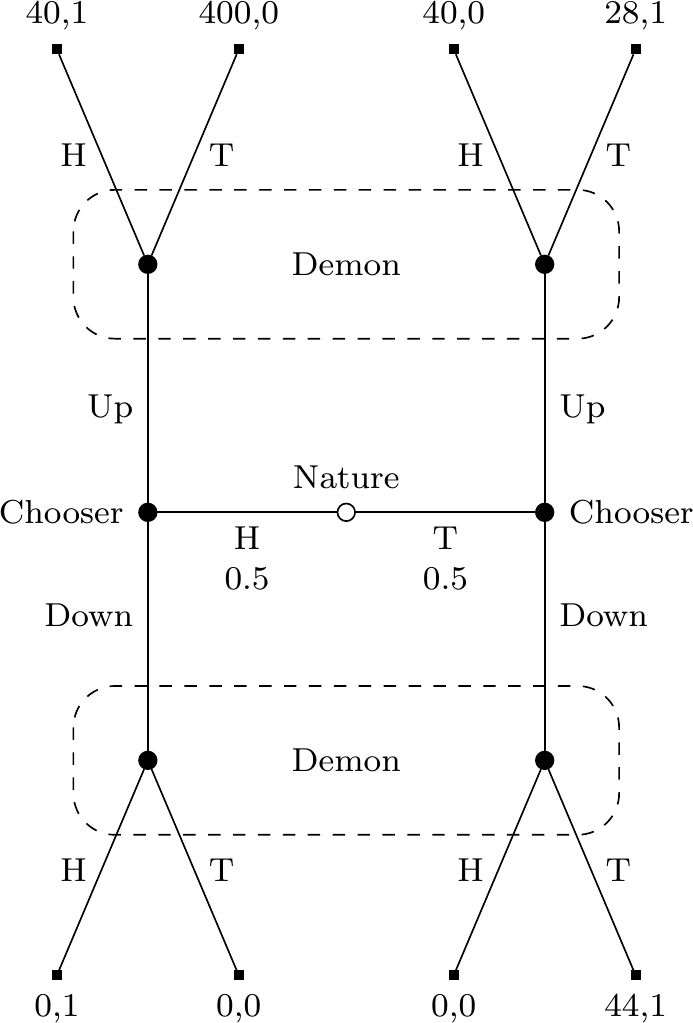
\includegraphics[width=0.6\textwidth,height=\textheight]{war-signal_files/figure-pdf/fig-second-anti-war-1.png}

}

\caption{\label{fig-second-anti-war}Tree Diagram of the Coins and
Signals Game}

\end{figure}

Demon predicts Chooser's strategy. That is, Demon predicts Chooser's
plan about what to do if the coin lands Heads and what to do if the coin
lands Tails, before the game starts. They make their guess about how the
coin landed after seeing Chooser's actual choice, and updating their
prior beliefs (about both the coin and Chooser) with this information.
If they predict that Chooser will do the same thing however the coin
lands, they will have no useful information about the coin, so they will
flip their own coin to make a guess. In that case it will be 50/50
whether Demon says Heads or Tails. Also, if Demon is surprised by what
Chooser does, i.e., if they had predicted Chooser would do one thing
however the coin lands but Chooser does the other thing, Demon will also
flip their own coin to make a guess.\footnote{A key part of the
  discussion in Cho and Kreps
  (\protect\hyperlink{ref-ChoKreps1987}{1987}) is that in some cases we
  can say substantive things about what a player will do if they are
  surprised in this sense. But Figure~\ref{fig-second-anti-war} is not
  such a case.} Finally, Demon's predictions are arbitrarily accurate.
For simplicity, I'll assume Demon is correct with probability 1, though
it doesn't matter if you allow for probability \(\varepsilon\) that
Demon gets it wrong.

Now I want to analyse what Chooser will do if they follow EDT. It should
be fairly clear that if the coin lands Heads, Chooser should say Up. The
worst possible return from Up is 40, the best possible return from Down
is 0. So that's what any theory would recommend, and Chooser will do
that whether or not they follow EDT. Indeed, this is so clear that we
should assume Demon will predict that Chooser will play Up if the coin
lands Heads. So what happens if the coin lands Tails? There are four
possibilities here: the two things Chooser might do crossed with the two
predictions Demon might make. The expected return to Chooser in these
four possibilities is given in Table~\ref{tbl-payout-if-tails}.

\hypertarget{tbl-payout-if-tails}{}
\begin{longtable}[]{@{}ccc@{}}
\caption{\label{tbl-payout-if-tails}The expected payout to Chooser in
four cases if the coin lands Tails}\tabularnewline
\toprule\noalign{}
& PUp & PDown \\
\midrule\noalign{}
\endfirsthead
\toprule\noalign{}
& PUp & PDown \\
\midrule\noalign{}
\endhead
\bottomrule\noalign{}
\endlastfoot
\textbf{Up} & 34 & 40 \\
\textbf{Down} & 18 & 44 \\
\end{longtable}

The numbers in Table~\ref{tbl-payout-if-tails} aren't entirely obvious;
I'll spell out how I got them.

\begin{itemize}
\tightlist
\item
  If Demon predicts Up (i.e., Demon predicts that Chooser will adopt a
  strategy that involves playing Up if the coin lands Heads) Demon will
  flip a coin. And they'll do that whatever Chooser does. That's because
  they'll either get no information (if Chooser plays Up), or will be
  surprised (if Chooser plays Down). So Chooser will get the average of
  lines 5 and 6 in Table~\ref{tbl-payoffs-demon-coin} if they play Up,
  and the average of lines 7 and 8 if they play Down.
\item
  If Demon predicts Down, and Chooser plays Up, Demon will think
  (falsely) that the coin must have landed Heads, since Demon will have
  predicted that Chooser will only say Up if Heads. So Demon will say
  Heads. So we'll definitely be at line 5 of
  Table~\ref{tbl-payoffs-demon-coin}, where Chooser gets 40.
\item
  If Demon predicts Down, and Chooser plays Down, Demon will think
  (correctly) that the coin must have landed Tails. So Demon will say
  that, and we'll be at line 8 of Table~\ref{tbl-payoffs-demon-coin}.
\end{itemize}

In a decision problem like Table~\ref{tbl-payout-if-tails}, EDT says
that all that matters is which of the top-left and bottom-right cells is
largest. In this case, it's the bottom-right, so EDT says to play Down.
That isn't absurd in this case; it gets the best possible payout of 44.
So that's our analysis of the game for EDT: Chooser plays Up if Heads,
Down if Tails, gets 40 if Heads and 44 if Tails (plus/minus a small
amount in expectation if Demon has \(\varepsilon\) chance of being
wrong), and on average gets 42.

GDT does not give any clear verdict about what to do in
Table~\ref{tbl-payout-if-tails}; it says either Up or Down is
permissible. So following GDT doesn't mean you'll do better than EDT in
this game; you might do exactly as well as EDT. But all it takes to get
a ``Why Ain'cha Rich?'' argument going is to show that one theory does
better than EDT. And the version of CDT that Dmitri Gallow
(\protect\hyperlink{ref-Gallow2020}{2020}) endorses implies that one
should play Up in Table~\ref{tbl-payout-if-tails}. So someone following
his theory will play Up however the coin lands. So Demon will always
flip a coin to decide what to do. So all of the top four outcomes in
Figure~\ref{fig-second-anti-war} are equally likely, and Chooser will on
average get a return of 127. Since 127~\textgreater~42, that means that
on average if Chooser follows Gallow's theory, they will on average be
much richer than if they follow EDT. So if ``Why Ain'Cha Rich?'', they
show that EDT should be rejected in favour of Gallow's theory.

Ian Wells (\protect\hyperlink{ref-Wells2019}{2019}) has earlier offered
an example where EDT predictably does worse than (all versions of) CDT.
His case involves a two-step game, where the EDTer will, at step 2, make
a decision that everyone, whether they believe in CDT or EDT or any
other plausible theory, think is bad from the perspective of the player
at step 1. At round 1 the players can pay to tie their hands at round 2,
and the EDTer will make this payment. (As would the CDTer who thinks
they will become an EDTer before round 2 starts.) Arif Ahmed
(\protect\hyperlink{ref-Ahmed2020}{2020}) responds that this is an
unfair criticism. In Wells's cases, he says, the EDT and CDT deciders
are not in equivalent situations in round one. The EDTer knows that they
will use EDT in later rounds, and the CDTer knows that they will use CDT
in later rounds. So they have different evidence about what will happen
at some later time in a way that's relevant to their current decision,
so it's not a like-for-like comparison between CDT and EDT at the first
stage.

I don't think this is a fair criticism of Wells, or a successful defence
of EDT. But even if you think Ahmed has shown how EDT survives Wells's
criticisms, his response doesn't work here. Chooser will definitely
choose Up if the coin lands Heads, whether they follow EDT, Gallow's
theory, or any remotely plausible theory. And this is common knowledge.
Demon knows this, and Chooser knows that Demon knows it, and so on. The
only difference is that if Chooser follows EDT, they will play Down if
Tails. And that's good as far as it goes; they'll probably get the
highest possible payoff they can get at that point. More importantly for
this debate, they will have the same subjective states if Tails is true
whether they follow EDT, Gallow's theory, or anything else. They will
believe that they would have played Up if Heads, and that the Demon
would have predicted that. So the different choices they make if the
coin lands Tails can't be traced back to differences in their subjective
states. So the complaint that Ahmed makes about Wells's examples can't
be made here (even setting aside the question of whether it is a fair
complaint). Nonetheless, the EDTer ends up with less money in the long
run than the follower of Gallow's theory when playing this game.

\hypertarget{sec-buchak}{%
\chapter{Risk-Weighted Utility}\label{sec-buchak}}

This appendix goes over a problem for Lara Buchak's risk-weighted
utility theory, based around the Single Choice Principle from
Chapter~\ref{sec-indecisive}. Buchak's theory concerns normal decision
problems, where there are no demons lying around, so we have to modify
Single Choice Principle a little to make it apply. The modifications
still leave it recognisably the same principle though. And the main
point of this appendix is to show that it is possible to theorise about
normal and abnormal decision problems using the same tools.

The core of Buchak's theory is a non-standard way of valuing a gamble.
For simplicity, we'll focus on gambles with finitely many outcomes.
Associate a gamble with a random variable \emph{O}, which takes values
\emph{o}\textsubscript{1}, \(\dots\), \emph{o\textsubscript{n}}, where
\emph{o\textsubscript{j}}~\textgreater~\emph{o\textsubscript{i}} iff
\emph{j}~\textgreater~\emph{i}. Buchak says that the risk-weighted
expected utility of \emph{O} is given by this formula, where \emph{r} is
the agent's risk-weighting function.

\[
REU(O) = o_1 + \sum_{i = 2}^n r(\Pr(O \geq o_i))(o_i - o_{i-1})
\]

The decision rule then is simple: choose the gamble with the highest
REU.

The key notion here is the function \emph{r}, which measures Chooser's
attitudes to risk. If \emph{r} is the identity function, then this
definition becomes a slightly non-standard way of defining expected
utility. Buchak allows it to be much more general. The key constraints
are that \emph{r} is monotonically increasing, that \emph{r}(0)~=~0 and
\emph{r}(1)~=~1. In general, if \emph{r}(\emph{x})~\textless~\emph{x},
Chooser is some intuitive sense more risk-averse than an expected
utility maximiser, while if \emph{r}(\emph{x})~\textgreater~\emph{x},
Chooser is more risk-seeking. The former case is more relevant to
everyday intuitions.

There are a number of good reasons to like Buchak's theory. Standard
expected utility theory explains risk-aversion in a surprisingly
roundabout way. Risk-aversion simply falls out as a consequence of the
fact that at almost all points, almost all goods have a declining
marginal utility. This is theoretically elegant - risk-aversion and
relative satiation are explained in a single framework - but has a
number of downsides. For one thing, it doesn't allow rational agents to
have certain kinds of risk-aversion, such as the kind described by
Allais (\protect\hyperlink{ref-Allais1953}{1953}). For another, it
doesn't seem like risk-aversion just is the same thing as the declining
marginal utility of goods. Buchak's theory, by putting attitudes to risk
into \emph{r}, avoids both these problems.

Unfortunately, Buchak's theory runs into problems. Our focus will be on
two-stage problems where Chooser's choice only makes a difference if the
game gets to stage 2. The general structure will be this.

\begin{enumerate}
\def\labelenumi{\arabic{enumi}.}
\tightlist
\item
  A coin with probability \emph{y} of landing Heads will be flipped. If
  it lands Tails, Chooser gets the Exit Payout, and the game ends.
\item
  If the game is still going, a second coin, with probability \emph{x}
  of landing Heads, will be flipped.
\item
  Chooser's payout will be a function of whether they chose Up or Down,
  and the result of this second coin.
\end{enumerate}

I'll write \emph{H}\textsubscript{1} and \emph{T}\textsubscript{1} for
the propositions that the first coin lands Heads and Tails respectively,
and \emph{H}\textsubscript{2} and \emph{T}\textsubscript{2} for the
propositions that the second coin lands Heads and Tails respectively.
I'll mostly be interested in the case where Up is a bet on
\emph{H}\textsubscript{2}, and Down is declining that bet, but the
general case is important to have on the table. The general structure of
these problems is given by Table~\ref{tbl-general-coin-exit}.

\begin{table}

\caption{\label{tbl-general-coin-exit}The abstract form of an exit
problem with coins.}\begin{minipage}[t]{0.50\linewidth}
\subcaption{\label{tbl-coin-exit-param}Exit Parameters}

{\centering 

\begin{tabular}[t]{cc}
\toprule
Exit Payout & \emph{e}\\
Pr(\emph{H}\textsubscript{1}) & \emph{y}\\
Pr(\emph{H}\textsubscript{2}) & \emph{x}\\
\bottomrule
\end{tabular}

}

\end{minipage}%
%
\begin{minipage}[t]{0.50\linewidth}
\subcaption{\label{tbl-coin-exit-r2g}Round 2 game}

{\centering 

\begin{tabular}[t]{ccc}
\toprule
 & \textbf{\emph{H}}\textsubscript{\textbf{2}} & \textbf{\emph{T}}\textsubscript{\textbf{2}}\\
\midrule
\textbf{Up} & \emph{a} & \emph{b}\\
\textbf{Down} & \emph{c} & \emph{d}\\
\bottomrule
\end{tabular}

}

\end{minipage}%

\end{table}

Then we get a version of Single Choice Principle that applies to games
like this.

\begin{itemize}
\tightlist
\item
  \textbf{Single Choice Principle}: Whether a choice is rational for
  Chooser is independent of whether Chooser chooses before or after they
  are told the result of the first coin flip.
\end{itemize}

Again, the argument for this turns on reflections about conditional
questions. If Chooser is asked before the first coin flip, they are
being asked what they want to do if the first coin lands Heads; if they
are asked after that flip, they are being asked what they want to do now
that the first coin landed Heads. These questions should get the same
answer. I'll show that REU-maximisation only gets that result if
\emph{r} is the identity function, i.e., if REU-maximisation just is
expected utility maximisation.

As before, I'll refer to Chooser's Early and Late choices, meaning their
choices before and after being told the result of the first coin. I'll
write \emph{REU\textsubscript{E}}(\emph{X}) to be the risk-weighted
expected utility of \emph{X} before finding out the result of the first
coin toss, and \emph{REU\textsubscript{L}}(\emph{X}) to be the
risk-weighted expected utility of \emph{X} after finding out the result
of the first coin toss. So Single Choice Principle essentially becomes
this biconditional, for any gambles \emph{X} and \emph{Y}.

\[
REU_E(X) \geq REU_E(Y) \leftrightarrow REU_L(X) \geq REU_L(Y)
\]

I'll first prove that this implies that \emph{r} must be multiplicative,
i.e., that \emph{r}(\emph{xy}) = \emph{r}(\emph{x})\emph{r}(\emph{y})
for all \emph{x}, \emph{y}. This isn't a particularly problematic
result; the most intuitive values for r, like r(x\emph{)~=}
x\textsuperscript{2}, are multiplicative. Consider the Exit Problem
shown in Table~\ref{tbl-zero-coin-exit}, where \emph{x} and \emph{y} are
arbitrary.

\begin{table}

\caption{\label{tbl-zero-coin-exit}An exit game with exit payout
0.}\begin{minipage}[t]{0.50\linewidth}
\subcaption{\label{tbl-zero-coin-exit-param}Exit Parameters}

{\centering 

\begin{tabular}[t]{cc}
\toprule
Exit Payout & 0\\
Pr(\emph{H}\textsubscript{1}) & \emph{y}\\
Pr(\emph{H}\textsubscript{2}) & \emph{x}\\
\bottomrule
\end{tabular}

}

\end{minipage}%
%
\begin{minipage}[t]{0.50\linewidth}
\subcaption{\label{tbl-zero-coin-exit-r2g}Round 2 game}

{\centering 

\begin{tabular}[t]{ccc}
\toprule
 & \textbf{\emph{H}}\textsubscript{\textbf{2}} & \textbf{\emph{T}}\textsubscript{\textbf{2}}\\
\midrule
\textbf{Up} & \(\frac{1}{r(x)}\) & 0\\
\textbf{Down} & 1 & 1\\
\bottomrule
\end{tabular}

}

\end{minipage}%

\end{table}

It's easy to check that
\emph{REU\textsubscript{L}}(\emph{U})~=~\emph{REU\textsubscript{L}}(\emph{D})~=~1.
So by Single Choice Principle,
\emph{REU\textsubscript{E}}(\emph{U})~=~\emph{REU\textsubscript{E}}(\emph{D}).
Since \emph{REU\textsubscript{E}}(\emph{U})~=~\(\frac{r(xy)}{r(x)}\),
and \emph{REU\textsubscript{L}}(\emph{D})~=~\emph{r}(\emph{y}), it
follows that \emph{r}(\emph{xy})~=~\emph{r}(\emph{x})\emph{r}(\emph{y}),
as required.

Define \emph{m}, for midpoint, as \emph{r}\textsuperscript{-1}(0.5).
Intuitively, \emph{m} is the probability where the risk-weighting agent
is indifferent between taking and declining a bet that stands to win and
lose the same amount. Since \emph{r} is monotonically increasing, and
goes from 0 to 1, \emph{m} must exist. Consider now
Table~\ref{tbl-one-coin-exit}, where \emph{y} is arbitrary.

\begin{table}

\caption{\label{tbl-one-coin-exit}An exit game with exit payout
1.}\begin{minipage}[t]{0.50\linewidth}
\subcaption{\label{tbl-one-coin-exit-param}Exit Parameters}

{\centering 

\begin{tabular}[t]{cc}
\toprule
Exit Payout & 1\\
Pr(\emph{H}\textsubscript{1}) & \emph{y}\\
Pr(\emph{H}\textsubscript{2}) & \emph{m}\\
\bottomrule
\end{tabular}

}

\end{minipage}%
%
\begin{minipage}[t]{0.50\linewidth}
\subcaption{\label{tbl-one-coin-exit-r2g}Round 2 game}

{\centering 

\begin{tabular}[t]{ccc}
\toprule
 & \textbf{\emph{H}}\textsubscript{\textbf{2}} & \textbf{\emph{T}}\textsubscript{\textbf{2}}\\
\midrule
\textbf{Up} & 2 & 0\\
\textbf{Down} & 1 & 1\\
\bottomrule
\end{tabular}

}

\end{minipage}%

\end{table}

In Table~\ref{tbl-one-coin-exit}, it's also easy to see that
\emph{REU\textsubscript{L}}(\emph{U})~=~\emph{REU\textsubscript{L}}(\emph{D})~=~1.
So by Single Choice Principle,
\emph{REU\textsubscript{E}}(\emph{U})~=~\emph{REU\textsubscript{E}}(\emph{D}).
And it's also clear that \emph{REU\textsubscript{E}}(\emph{D})~=~1,
since that's the only possible payout for Down. So
\emph{REU\textsubscript{E}}(\emph{U})~=~1. So we get the following
result.

\begin{align*}
REU_E(U) &= r(1-y(1-m)) + r(ym) \\
 &= 1    \\
\therefore  r(1-y(1-m)) &= r(ym)
\end{align*}

That doesn't look like a particularly notable result, but it will become
useful when we discuss our last case, Table~\ref{tbl-two-coin-exit},
which is just the same as Table~\ref{tbl-one-coin-exit}, except the exit
payout is now 2.

\begin{table}

\caption{\label{tbl-two-coin-exit}An exit game with exit payout
2.}\begin{minipage}[t]{0.50\linewidth}
\subcaption{\label{tbl-two-coin-exit-param}Exit Parameters}

{\centering 

\begin{tabular}[t]{cc}
\toprule
Exit Payout & 2\\
Pr(\emph{H}\textsubscript{1}) & \emph{y}\\
Pr(\emph{H}\textsubscript{2}) & \emph{m}\\
\bottomrule
\end{tabular}

}

\end{minipage}%
%
\begin{minipage}[t]{0.50\linewidth}
\subcaption{\label{tbl-two-coin-exit-r2g}Round 2 game}

{\centering 

\begin{tabular}[t]{ccc}
\toprule
 & \emph{H}\textsubscript{2} & \emph{T}\textsubscript{2}\\
\textbf{Up} & 2 & 0\\
\textbf{Down} & 1 & 1\\
\bottomrule
\end{tabular}

}

\end{minipage}%

\end{table}

In Table~\ref{tbl-two-coin-exit}, it's again easy to see that
\emph{REU\textsubscript{L}}(\emph{U})~=~\emph{REU\textsubscript{L}}(\emph{D})~=~1.
So by Single Choice Principle,
\emph{REU\textsubscript{E}}(\emph{U})~=~\emph{REU\textsubscript{E}}(\emph{D}).
But the early values are more complicated:
\emph{REU\textsubscript{E}}(\emph{D})~=~1~+~\emph{r}(1-\emph{y}), and
\emph{REU\textsubscript{E}}(\emph{U})~=~2\emph{r}(1-\emph{y}(1-\emph{m})).
Using what we've discovered so far, we can do something with that last
value.

\begin{align*}
REU_E(U) &= 2r(1-y(1-m)) \\
  &= 2(1-r(ym))  && \text{from previous calculations} \\
  &= 2 - 2r(ym) \\
  &= 2 - 2r(y)r(m) && \text{since $r$ is multiplicative} \\
  &= 2 - r(y)  && \text{since $r(m) = 0.5$}
\end{align*}

Putting all this together, we get

\begin{align*}
REU_E(D) &= REU_E(U)  && \Rightarrow \\
1 + r(1-y) &= 2 - r(y) && \Rightarrow \\
r(y) + r(1-y) &= 1
\end{align*}

So \emph{r} is a monotonic increasing function satisfying
\emph{r}(0)~=~0, \emph{r}(1)~=~1,
\emph{r}(\emph{xy})~=~\emph{r}(\emph{x})\emph{r}(\emph{y}), and
\emph{r}(\emph{y})~+~\emph{r}(1-\emph{y})~=~1. The only such function is
\emph{r}(\emph{x})~=~\emph{x}. So the only version of risk-weighted
expected utility theory that satisfies Single Choice Principle is where
\emph{r}(\emph{x})~=~\emph{x}, i.e., where risk-weighted expected
utility just is old-fashioned expected utility.

This doesn't yet prove expectationism. I haven't shown that there is no
other alternative to expected utility theory that satisfies Single
Choice Principle. There are such other theories out there, such as the
Weighted-linear utility theory described by Bottomley and WIlliamson
(\protect\hyperlink{ref-BottomleyWilliamsonnd}{n.d.}). But it's a guide
to how we could start defending expectationism in a way consistent with
how we handle decision problems involving demons.

\hypertarget{sec-unique}{%
\chapter{Against Uniqueness}\label{sec-unique}}

In setting out GDT, I said that what mattered was that Chooser maximised
expected utility given some credal function that was rational having
made their choice. Some philosophers argue that the quantifier in the
previous sentence is redundant; there is only one rational credence
function one could have given some evidence. This view is known as
Uniqueness, and its negation is known as Permissivism. The way I've
stated GDT presupposes that Permissivism is correct, and I should defend
that presupposition.

This appendix argues that thinking about symmetric games gives us new
reason to believe in Permissivism. In keeping with the spirit of the
book, the arguments will be game-theoretic. I'm going to offer two
arguments, one involving finite games, and the other involving infinite
games. In finite games, the theorist who denies Permissivism says that
the players have to think that the other player is more likely to take
one action rather than another, although they know the actions have
equal expected utility. In infinite games, the theorist who denies
Permissivism has to say that it is impossible for certain games to be
played with common knowledge of rationality and shared evidence,
although there does not seem to be anything paradoxical about the games.
The latter set of arguments rely on the recent discovery that there are
symmetric games with only asymmetric equilibria. It was long known that
there are symmetric games with no pure strategy symmetric equilibria;
the surprising new discovery is that there are symmetric games with
asymmetric equilibria, but no symmetric equilibria involving either
mixed or pure strategies. In both cases, thinking about players in
symmetric games pushes us towards accepting Permissivism.

The Permissivist theses that have been the focus on recent philosophical
attention vary along two dimensions.\footnote{For a much more thorough
  introduction to the debate, and especially into the varieties of
  Permissivist theses, see Kopec and Titelbaum
  (\protect\hyperlink{ref-KopecTitelbaum2016}{2016}) and Meacham
  (\protect\hyperlink{ref-Meacham2019}{2019}). The next three paragraphs
  draw heavily from these two papers. For more recent arguments in
  favour of Permissivism, see Callahan
  (\protect\hyperlink{ref-Callahan2021}{2021}), Lota and Hlobil
  (\protect\hyperlink{ref-Lota2023}{2023}), Palmira
  (\protect\hyperlink{ref-Palmira2023}{2023}), and Ye
  (\protect\hyperlink{ref-Ye2023}{2023}). For criticisms, see Schultheis
  (\protect\hyperlink{ref-Schultheis2018}{2018}) and Ross
  (\protect\hyperlink{ref-Ross2021}{2021}).}

The first dimension concerns what we hold fixed when we say that
multiple attitudes are rationally permissible. It's basically common
ground that people with different evidence can rationally believe
different things, or that a person can believe different things when
their evidence changes. But are these sufficient conditions for rational
disagreement or change also necessary conditions. What's called
\emph{Interpersonal Permissiveness} says that given some evidence, there
may be more than one doxastic state that it is rational to be
in.\footnote{In setting up the debate, I'm following the standard
  practice and assuming some kind of evidentialism. If one thinks that
  other things than evidence matter to rational credence, such as
  thinking that testimony provides non-evidential reasons for belief, it
  is a little complicated but possible to restate everything here to fit
  such an epistemological view. The general picture is that `evidence'
  here really means non-pragmatic reasons for belief. But it's simpler
  to say `evidence', and that's what I'll generally say.} What's called
\emph{Intrapersonal Permissiveness} says that given a person and some
evidence, there may be more one doxastic state that it is rational to be
in. A classic form of subjectivist Bayesianism says that a person can
pick any prior they like, but they have to update it by
conditionalisation. This is a version of a view that rejects
Intrapersonal Permissiveness, since given one's prior there is only one
permissible posterior, but endorses Interpersonal Permissiveness, since
there are multiple permissible priors.

The second dimension concerns whether the distinct views can be
acknowledged as rational. Stewart Stewart Cohen
(\protect\hyperlink{ref-Cohen2013}{2013}) defends the view that multiple
attitudes can be rational, but one cannot rationally acknowledge a
distinct view as rational. Following Kopec and Titelbaum
(\protect\hyperlink{ref-KopecTitelbaum2016}{2016}), call a view that
says multiple views can both be rationally held and be believed to be
rational \emph{Acknowledged Permissiveness}, and the view that says
multiple views could be rationally held, but could not be acknowledged,
\emph{Unacknowledged Permissiveness}.

Putting the last two paragraphs together gives us four varieties of
Permissive theses. The negation of a Permissive thesis is a Uniqueness
thesis. The name suggests that there is precisely one rational attitude
to take in a specified situation, but we'll interpret it as the view
that there is at most one rational attitude to take so as to ensure each
Uniqueness thesis is the negation of a Permissive thesis. So if there
are four Permissive theses, there are four Uniqueness theses that negate
them.

This appendix focuses on the strongest of these four Permissive theses,
Acknowledged Intrapersonal Permissiveness, and its negation,
Acknowledged Interpersonal Uniqueness. This is, I think, the most
commonly discussed form of Permissiveness in the literature, and in any
case is interesting. And I'm going to be arguing that in some cases
involving symmetric games, coherence considerations provide a strong
argument in favour of Acknowledged Intrapersonal Permissiveness.

The next two sections set out two symmetric games where
Uniqueness\footnote{From now on, when I say `Uniqueness' I mean
  Acknowledged Intrapersonal Uniqueness. It's easier to simply stipulate
  this now than repeating the phrase every time.} leads to surprising
results. In all cases I'll assume that if Uniqueness is true, then the
players know that it is true. And while this might be obvious, I'll also
note explicitly that they players have no evidence about the game or the
players beyond what I write about the structure of the games.

\hypertarget{chicken}{%
\section{Chicken}\label{chicken}}

Some finite symmetric games don't have a symmetric pure-strategy
equilibrium. One notable example is Chicken, one version of which is in
Table~\ref{tbl-unique-chicken}.

\hypertarget{tbl-unique-chicken}{}
\begin{longtable}[]{@{}ccc@{}}
\caption{\label{tbl-unique-chicken}Chicken}\tabularnewline
\toprule\noalign{}
& \textbf{Stay} & Swerve \\
\midrule\noalign{}
\endfirsthead
\toprule\noalign{}
& \textbf{Stay} & Swerve \\
\midrule\noalign{}
\endhead
\bottomrule\noalign{}
\endlastfoot
\textbf{Stay} & -100,-100 & 1, -1 \\
\textbf{Swerve} & -1, 1 & 0, 0 \\
\end{longtable}

The symmetric pure-strategy pairs (Stay, Stay) and (Swerve, Swerve) are
not equilibria; in each case both parties have an incentive to defect.
But the game does have a symmetric mixed strategy equilibrium. It is
that both players play the mixed strategy of Stay with probability 0.01,
and Swerve with probability 0.99.

Now assume that Row and Column have the same relevant evidence, that
they are self-aware and fully rational, and that these facts and no
other are common knowledge between them, and that they are about to play
Chicken one time. (It's also common knowledge that they won't play
again; dropping this would raise the possibility of complicated
strategic reasoning.)

Let \textbf{Swerve} be the proposition that a rational player with that
evidence will Swerve. And call the players Row and Column. Given our
assumptions so far, plus Uniqueness, we can prove that Row's credence in
\textbf{Swerve} is 0.99. Here's the proof.

\begin{enumerate}
\def\labelenumi{\arabic{enumi}.}
\tightlist
\item
  Let \emph{x} be Row's credence in \textbf{Swerve}.
\item
  By self-awareness, Row knows that \emph{x} is her credence in
  \textbf{Swerve}.
\item
  Since Row knows Row is rational, Row can infer that \emph{x} is a
  rational credence in \textbf{Swerve}.
\item
  Since Row knows Uniqueness is true, Row can infer that \emph{x} is the
  only rational credence in \textbf{Swerve}.
\item
  Since Row knows Column is rational, Row can infer that \emph{x} is
  Column's credence in \textbf{Swerve}, since (at step 4) Row has
  deduced that \emph{x} is the only rational credence in
  \textbf{Swerve}.
\item
  Since all the assumptions so far are common knowledge, Row can come to
  know that Column knows that \emph{x} is Row's credence in
  \textbf{Swerve}.
\item
  If \emph{x} = 1, then Row can come to know that it is rational for
  Column to Swerve, while knowing that Row will also Swerve. But this is
  impossible, since if Column knows Row will Swerve, it is best for
  Column to Stay. So \emph{x} ≠ 1.
\item
  If \emph{x} = 0, then Row can come to know that it is rational for
  Column to Stay, while knowing that Row will also Stay. But this is
  impossible, since if Column knows Row will Stay, it is best for Column
  to Swerve. So \emph{x} ≠ 0.
\item
  So 0 \textless{} \emph{x} \textless{} 1.
\item
  Since Row knows Column's credence that Row will Swerve (as was shown
  at step 6), and Row knows Column is rational, but Row does not know
  what Column will do, it must be that Column is indifferent between
  Stay and Swerve given her (i.e., Column's) credences about what Row
  will do.\footnote{If Column was not indifferent between their options,
    the knowledge Row has by step 6 would be sufficient to deduce with
    certainty what Column will do. But at step 9 we showed that Row does
    not know what Column will do.}
\item
  Column is indifferent between Stay and Swerve only if her credence
  that Row will Swerve is 0.99. (This is a reasonably simple bit of
  algebra to prove.)
\item
  So from 10 and 11, Column's credence that Row will Swerve is 0.99.
\item
  By (known) Uniqueness, it follows that the only rational credence in
  \textbf{Swerve} is 0.99.
\item
  So since Row is rational, it follows that \emph{x} = 0.99.
\end{enumerate}

Now there is nothing inconsistent in this reasoning. In a sense, it is
purely textbook reasoning. But the conclusion is deeply puzzling. We've
proven that Column is indifferent between her two options. And we've
proven that Row knows this. But we've also proven that Row thinks it is
99 times more likely that Column will choose one of the options over the
other. Why is that? It isn't because there is more reason to do one than
the other; given Column's attitudes, the options are equally balanced.
It is purely because Uniqueness pushes us to a symmetric equilibrium,
and this is the only symmetric equilibrium. Given Uniqueness, the only
coherent state is to have believe the other party is 99 times more
likely to resolve a tie one way rather than another.

It's important here that we're imagining a one-shot version of Chicken.
If the game is played repeatedly, then it is natural that the players
will tend to the equilibrium of the game. What is surprising is that
Uniqueness pushes us to thinking that, if the rationality of the players
is common knowledge, the mixed strategy Nash equilibrium will be played
in a one-shot game. As Matthias Risse
(\protect\hyperlink{ref-Risse2000}{2000}) argues, the argument that
mixed strategy Nash equilibria are rational requirements of one-shot
games is very weak. But it's a conclusion the Uniqueness theorist is
forced into.

It's even more puzzling because of another feature of Uniqueness. It's
often very hard to see what the uniquely rational attitude could be in
cases where the evidence is very sparse. The usual way to resolve this
problem is to appeal to what Keynes
(\protect\hyperlink{ref-Keynes1921}{1921}) dubbed the Principle of
Indifference. That principle says, roughly, that if the evidence
available for two options is equally good, treat them as equally likely.
Here, Row thinks that Column is a utility maximiser who has two options
of equal utility available to them. And Row concludes (and must conclude
if Uniqueness is correct) that one of these options is 99 times more
likely to be played. That's not inconsistent with the letter of the
Principle of Indifference. But it is inconsistent with the spirit of it.

All that said, I suspect many defenders of Uniqueness will be happy to
accept these conclusions. The next case is I think poses a deeper
problem for them.

\hypertarget{elections}{%
\section{Elections}\label{elections}}

The cases in this section come from some recent work on a rather old
question,

\begin{quote}
If a symmetric game has an equilibrium, does it have a symmetric
equilibrium?
\end{quote}

Over the years, a positive answer was given to various restricted forms
of that question. Most importantly, John Nash
(\protect\hyperlink{ref-Nash1951}{1951}) showed that if each player has
finitely many moves available, then the game does have a symmetric
equilibrium.

But recently it has been proven that the answer to the general question
is no. Mark Fey (\protect\hyperlink{ref-Fey2012}{2012}) describes an
example of a positive-sum two-player game that has only asymmetric
equilibria.\footnote{In Fey's game both players pick a real in {[}0,
  1{]}. If both players pick numbers in (0, 1), the one who picks the
  larger number wins. But there are a lot of complications if one or
  both pick an extreme value, including the game not always being
  zero-sum. I'm not relying on it here because it is a little too close
  to the game I'll discuss at the end of this section where everyone
  agrees there is no way to play it given common knowledge of
  rationality. Fey's paper also includes a nice chronology of some of
  the proofs of positive answers to restricted forms of the question.}
Dimitrios Xefteris (\protect\hyperlink{ref-Xefteris2015}{2015}) showed
that there is a symmetric three-player zero-sum game that has only
asymmetric equilibria. In fact, he showed that a very familiar game, a
version of a Hotelling--Downs model of elections, has this property.
Here's how he describes the game.

\begin{quote}
Consider a unit mass of voters. Each voter is characterised by her ideal
policy. We assume that the ideal policies of the voters are uniformly
distributed in {[}0, 1{]}. We moreover assume that three candidates
\emph{A}, \emph{B} and \emph{C} compete for a single office. Each
candidate \emph{J} \(\in\) \{\emph{A}, \emph{B}, \emph{C}\} announces a
policy \emph{s\textsubscript{J}} \(\in\) {[}0, 1{]} and each voter votes
for the candidate who announced the policy platform which is nearest to
her ideal policy. If a voter is indifferent between two or among all
three candidates she evenly splits her vote between/among them. A
candidate \emph{J} \(\in\) \{\emph{A}, \emph{B}, \emph{C}\} gets a
payoff equal to one if she receives a vote-share strictly larger than
the vote-share of each of the two other candidates. If two candidates
tie in the first place each gets a payoff equal to one half. If all
three candidates receive the same vote-shares then each gets a payoff
equal to one third. In all other cases a candidate gets a payoff equal
to zero. (\protect\hyperlink{ref-Xefteris2015}{Xefteris 2015, 124})
\end{quote}

It is clear that there is no symmetric pure-strategy equilibrium here.
If all candidates announced the same policy, everyone would get a payoff
of \(\frac{1}{3}\). But no matter what that policy is, if \emph{B} and
\emph{C} announce the same policy, then \emph{A} has a winning move
available. (If the number \emph{B} and \emph{C} say is not 0.5, \emph{A}
wins by saying 0.5. If they do both say 0.5, then \emph{A} wins by
saying 0.4.)

What's more surprising, and what Xefteris proves, is that there is no
symmetric mixed strategy equilibria either. Again, in such an
equilibrium, any player would have a payoff of \(\frac{1}{3}\). Very
roughly, the proof that no such equilibrium exists is that random
deviations from the equilibrium are as likely to lead to winning as
losing, so they have a payoff of roughly \(\frac{1}{2}\). So there is no
incentive to stay in the equilibrium. So no symmetric equilibrium
exists.

Using this game, I'm going to offer the following argument for
Uniqueness.

\begin{enumerate}
\def\labelenumi{\arabic{enumi}.}
\tightlist
\item
  It's possible that three people can play this (symmetric) game in a
  situation where it is commonly known that (a) each of them is
  rational, and (b) they have the same evidence. In the relevant sense
  of `rational' a person is rational iff they have credences that are
  supported by their evidence, and they perform actions that maximise
  expected utility given their credences.
\item
  If Uniqueness is true, then in a symmetric game where it is common
  knowledge that each person has the same evidence and is rational,
  every player will believe that the others have the same credences
  about what the others will do.
\item
  If premise 2 is true, then if the players have the same evidence and
  are rational, the result of the game will be a symmetric equilibrium.
\item
  The game does not have a symmetric equilibrium.
\item
  So Uniqueness is false.
\end{enumerate}

I'll go over this abstract argument, then apply it to the Xefteris game.

Premise 1 is a claim that a particular game, that has an equilibrium, is
possible to play. There is a strong assumption that mathematically
coherent games are indeed possible to play, so this feels like a safe
enough assumption. I'll come back at the very end of the next section to
whether it is safe.

Premise 2 is spelling out a consequence of Uniqueness, but it helps to
go over why it is a consequence. Assume that player \emph{x} has
credence \emph{p} that player \emph{y} will play (pure) strategy
\emph{s}. In symbols,
\emph{Cr\textsubscript{x}}(\emph{s\textsubscript{y}}) = \emph{p}, where
\emph{Cr\textsubscript{x}} is \emph{x}'s credence function, and
\emph{s\textsubscript{y}} is the proposition that \emph{y} plays
strategy \emph{s}. By common knowledge of rationality, \emph{x} thinks
it is rational with their evidence to have credence \emph{p} in
\emph{s\textsubscript{y}}. By Uniqueness, \emph{x} thinks this is the
only rational credence to have in \emph{s\textsubscript{y}}. By common
knowledge of sameness of evidence, \emph{x} thinks that \emph{y} is
rational, and has the same evidence about \emph{x} playing \emph{s} as
\emph{x} has about \emph{y} playing \emph{s}. So \emph{y} will do the
only rational thing with that evidence, namely form credence \emph{p}
that \emph{x} will play \emph{s}. (In a game with more than two players,
this also licences inferring that \emph{y} believes that \emph{z} will
play \emph{s} with probability \emph{p}, and the same for all the other
players.) Quite generally, \emph{x} believes that \emph{y} has the same
credences about \emph{x} as \emph{x} themselves has about \emph{y}.

Premise 3 says that this suffices for there to be a symmetric
equilibrium of the game. In fact, we can say what that equilibrium would
be: everyone plays the mixed strategy that corresponds to \emph{x}'s
credences about what \emph{y} will play. By 'mixed strategy
corresponding to these credences, I mean that if
\emph{Cr\textsubscript{x}}(\emph{s\textsubscript{y}}) = \emph{p}, then
each player \emph{y} in fact plays strategy \emph{s} with probability
\emph{p}, and so on for all strategies, and probabilities.

Why is that strategy set, where everyone does what \emph{x} thinks
\emph{y} will do, an equilibrium? It starts with the fact that premise
2, and the reasoning behind it, is all a priori. So it's knowable to a
perfectly rational player, like \emph{x}. So, if Uniqueness is true,
\emph{x} knows that whatever they think about the other players will (a)
be true, and (b) be common knowledge. And since \emph{x} takes the other
players to be utility maximisers, that means that every strategy
\emph{x} gives them positive probability of playing must maximise
expected utility given these (shared) credences about what everyone else
will play. If there was some strategy that did not maximise expected
utility, and \emph{x} gave them positive probability of playing it, then
\emph{x} would think it was possible that the other player was not
maximising expected utility, contradicting the assumption of common
knowledge of rationality. That's to say, playing the mixed strategy that
corresponds to \emph{x}'s beliefs about \emph{y} must be an equilibrium,
if Uniqueness is true, and it is common knowledge that the players have
the same evidence and are rational.

Premise 4 says that something which is entailed by Uniqueness, combined
with the assumptions in premise 1 and the other two premises, is not in
fact true. So by modus tollens, Uniqueness is not true.

The arguments about the first three premises should apply to any
symmetric game, with common knowledge of rationality and shared
evidence. In any such game, the credences any player has about any other
should be convertible into a (possibly mixed) equilibrium of the game.
That's because any player should be able to conclude that what they
think about one player must be a rational belief (by the common
knowledge of rationality), so must be the only rational belief given
their own evidence (by Uniqueness), so must be the belief that everyone
has (by shared evidence), so must in fact be correct (since it's the
only rational belief, and they are rational), and since it is a correct
belief, and everyone is in fact a utility maximiser while holding these
(correct) beliefs about everyone, must be an equilibrium. So every
symmetric game must have a symmetric equilibrium, if Uniqueness is true,
and the game is played under conditions of common knowledge of
rationality and shared evidence.

That's not true in this game. It does not in fact have a symmetric
equilibrium. If we drop Uniqueness, it is easy enough to describe
rational behaviour for players in this game. Here is one possible model
for the game.

\begin{itemize}
\tightlist
\item
  \emph{A} plays 0.6 (and wins), \emph{B} and \emph{C} each play 0.4
  (and lose).
\item
  Each player has a correct belief about what the other players will
  play.
\item
  But both \emph{B} and \emph{C} know they cannot win given the other
  player's moves, so they pick a move completely arbitrarily.
\item
  Further, each player has a correct belief about why each player makes
  the move they make.
\end{itemize}

This is the coherent equilibria that Xefteris describes, but it requires
some amount of luck, since it requires that \emph{B} and \emph{C} pick
0.4 when they could pick absolutely anything. Here's a slightly more
plausible model of the game.

\begin{itemize}
\tightlist
\item
  \emph{A} plays 0.6 (and wins), \emph{B} and \emph{C} each play 0.4
  (and lose).
\item
  The only two rational plays are 0.4 and 0.6, and each of them is
  rationally permissible.
\item
  In any world that a player believes to be actual, or a player believes
  another player believes to be actual, or a player believes another
  player believes another player believes to be actual, etc., the
  following two conditions hold.
\item
  If a player plays 0.6, they believe the other two players will play
  0.4, and hence playing 0.6 is a winning move.
\item
  If a player plays 0.4, they believe the other two players will play
  0.6, and hence playing 0.4 is a winning move.
\end{itemize}

The main difference between this model and Xefteris's is that it allows
that players have false beliefs. But why shouldn't they have false
beliefs? All they know is that the other players are rational, and
rationality (we're assuming) does not settle a unique verdict for what
players will do. So I think this strategy set, where the players have
rational (but false) beliefs about the other players, is more useful to
think about.

\hypertarget{objections}{%
\section{Objections}\label{objections}}

The arguments for premises 2 and 3 in the argument above assumed
something slightly stronger than Uniqueness. They each assumed that each
player knew Uniqueness was true, and could use that in their reasoning.
(Most importantly, in the argument for premise 3, it's important that
each player can reason through the reasoning behind premise 2, and that
reasoning used Uniqueness.) What happens if we drop that assumption, and
consider the possibility that Uniqueness is true but unknowable?

This possibility is a little uncomfortable for philosophical defenders
of Uniqueness. If the players in these games do not know that Uniqueness
is true, then neither do the authors writing about Uniqueness. And now
we have to worry about whether it is permissible to assert in print that
Uniqueness is true. I wouldn't make too much of this though. It is
unlikely that a knowledge norm governs assertion in philosophical
journals.

The bigger worry here is that one key argument for Uniqueness seems to
require that Uniqueness is knowable. A number of recent authors have
argued that Uniqueness best explains our practice of deferring to
rational people.\footnote{There is a nice discussion of this argument,
  including citations of the papers I'm about to discuss, in Kopec and
  Titelbaum (\protect\hyperlink{ref-KopecTitelbaum2016}{2016, 195}).}
For instance, Greco and Hedden use this principle in their argument for
Uniqueness.

\begin{quote}
If agent \emph{S}\textsubscript{1} judges that
\emph{S}\textsubscript{2}'s belief that \emph{P} is rational and that
\emph{S}\textsubscript{1} does not have relevant evidence that
\emph{S}\textsubscript{2} lacks, then \emph{S}\textsubscript{1} defers
to \emph{S}\textsubscript{2}'s belief that \emph{P}.
(\protect\hyperlink{ref-GrecoHedden2016}{Greco and Hedden 2016, 373}).
\end{quote}

Similar kinds of arguments are made by Dogramaci
(\protect\hyperlink{ref-Dogramaci2012}{2012}) and Horowitz
(\protect\hyperlink{ref-Horowitz2014}{2014}). But the principle looks
rather dubious in the case of these games. Imagine that \emph{A} forms a
belief (we'll come back to how) that \emph{B} believes that a rational
thing to do in the Xefteris game is to play 0.6, and so believes that
\emph{B} will play 0.6. This last step requires Uniqueness, or, more
specifically, \emph{A}'s belief that \emph{B} believes in Uniqueness.
The reasoning is as follows. \emph{A} thinks that \emph{B} thinks that
0.6 is a rational move; so, by Uniqueness, \emph{A} believes that
\emph{B} believes that 0.6 is the only rational move; so, by \emph{B}'s
belief in their own rationality, \emph{B} believes that they will play
0.6; so, by \emph{B}'s self-control as a practically rational agent,
\emph{B} will in fact play 0.6. Now \emph{A} believes that they have the
same evidence as \emph{B}, and that a rational thing to do with that
evidence is play 0.6. By Uniqueness, they will believe that the only
rational thing for someone with the evidence that they have (and that
\emph{B} has) is to play 0.6. But that can't be right. If \emph{B} is
playing 0.6, as \emph{A} has independently judged they will, the
rational thing for \emph{A} to do is to play something other than 0.6.

And that's the general case for these symmetric games with only
asymmetric equilibria. Believing that someone else is at an equilibrium
point is a reason to not copy them. Uniqueness, combined with common
knowledge of shared evidence and rationality, implies that anyone who
believes that another player will adopt strategy \emph{s} has a reason
to adopt strategy \emph{s}. After all, another player is playing it, and
since that player is rational it is a rational thing to do in their
situation, so by common evidence it is a rational thing to do in one's
own situation, so by Uniqueness it is the only rational thing to do in
one's own situation. But since the symmetric situations are not
equilibria, believing that the other person will do \emph{s} cannot be a
reason to do \emph{s}. That means one of the three assumptions we made
here - common knowledge of rationality, common knowledge of shared
evidence, and Uniqueness, must be wrong. Since it is typically taken to
be at least coherent to have common knowledge of rationality and common
knowledge of shared evidence, it follows that Uniqueness is wrong.

But maybe the Uniqueness theorist could resist that last step. Maybe
they could deny that the game, with the assumption of common knowledge
of rationality and shared evidence, really is possible. \footnote{This
  move won't really help with Chicken; but maybe in that case they can
  simply insist that a rational player will rationally think the other
  player is more likely to make one of the two choices with equal
  expected payoffs.} This perhaps isn't as surprising as it might seem.

Note two things about the Xefteris game. First, it is an infinite game
in the sense that each player has infinitely many choices. It turns out
this matters to the proof that there is no symmetric equilibrium to the
game. Second, we are assuming it is common knowledge, and hence true,
that the players are perfectly rational. Third, we are assuming that
perfect rationality entails that people will not choose one option when
there is a better option available. When you put those three things
together, some things that do not look obviously inconsistent turn out
to be impossible. Here's one example of that.

\begin{quote}
\emph{A} and \emph{B} are playing a game. Each picks a real number in
the open interval (0, 1). They each receive a payoff equal to the
average of the two numbers picked.
\end{quote}

For any number that either player picks, there is a better option
available. It is always better to pick \(\frac{x+1}{2}\) than \emph{x},
for example. So it is impossible that each player knows the other is
rational, and that rationality means never picking one option when a
better option is available.

So the Uniqueness theorist could say that the same thing is going on in
the Xefteris game. Some infinitely games cannot be played by rational
actors (understood as people who never choose sub-optimal options); this
is one of them. But if this is all the Uniqueness theorist says, it is
not a well motivated response. We can say why it is impossible to
rationally play games like the open interval game; the options get
better without end. But that isn't true in the Xefteris game. The only
thing that makes the game seem impossible is the Uniqueness assumption.
People who reject Uniqueness can easily describe how the Xefteris game
can be played by rational players. Simply saying that it is impossible,
without any motivation or explanation for this other than Uniqueness
itself, feels like an implausible move.

\hypertarget{conclusion}{%
\section{Conclusion}\label{conclusion}}

If Uniqueness is true, then the following thing happens in games between
people who know each other to have the same evidence, and to be
rational. When someone forms a belief about what the other person will
do, they can infer that this is a rational way to play the game given
knowledge that everyone else will do the same thing. But sometimes this
is a very unintuitive inference. In Chicken, it implies that we should
have asymmetric attitudes to someone who is facing a choice between two
options with equal expected value. In the election game Xefteris
describes, a game that feels consistent turns out to be impossible.

I think the conclusion to draw from these cases of symmetric
interactions this is that Uniqueness is false, and hence Permissivism is
true. Sometimes in such an interaction one simply has to form a belief
about the other player, knowing they may well form a different belief
about you. Indeed, sometimes only coherent way to form a belief about
the other player is to believe that they will form a different belief
about you. And that means giving up on Uniqueness.



\end{document}
